\documentclass[aspectratio=169]{beamer}\usepackage[]{graphicx}\usepackage[]{xcolor}
% maxwidth is the original width if it is less than linewidth
% otherwise use linewidth (to make sure the graphics do not exceed the margin)
\makeatletter
\def\maxwidth{ %
  \ifdim\Gin@nat@width>\linewidth
    \linewidth
  \else
    \Gin@nat@width
  \fi
}
\makeatother

\definecolor{fgcolor}{rgb}{0.345, 0.345, 0.345}
\newcommand{\hlnum}[1]{\textcolor[rgb]{0.686,0.059,0.569}{#1}}%
\newcommand{\hlsng}[1]{\textcolor[rgb]{0.192,0.494,0.8}{#1}}%
\newcommand{\hlcom}[1]{\textcolor[rgb]{0.678,0.584,0.686}{\textit{#1}}}%
\newcommand{\hlopt}[1]{\textcolor[rgb]{0,0,0}{#1}}%
\newcommand{\hldef}[1]{\textcolor[rgb]{0.345,0.345,0.345}{#1}}%
\newcommand{\hlkwa}[1]{\textcolor[rgb]{0.161,0.373,0.58}{\textbf{#1}}}%
\newcommand{\hlkwb}[1]{\textcolor[rgb]{0.69,0.353,0.396}{#1}}%
\newcommand{\hlkwc}[1]{\textcolor[rgb]{0.333,0.667,0.333}{#1}}%
\newcommand{\hlkwd}[1]{\textcolor[rgb]{0.737,0.353,0.396}{\textbf{#1}}}%
\let\hlipl\hlkwb

\usepackage{framed}
\makeatletter
\newenvironment{kframe}{%
 \def\at@end@of@kframe{}%
 \ifinner\ifhmode%
  \def\at@end@of@kframe{\end{minipage}}%
  \begin{minipage}{\columnwidth}%
 \fi\fi%
 \def\FrameCommand##1{\hskip\@totalleftmargin \hskip-\fboxsep
 \colorbox{shadecolor}{##1}\hskip-\fboxsep
     % There is no \\@totalrightmargin, so:
     \hskip-\linewidth \hskip-\@totalleftmargin \hskip\columnwidth}%
 \MakeFramed {\advance\hsize-\width
   \@totalleftmargin\z@ \linewidth\hsize
   \@setminipage}}%
 {\par\unskip\endMakeFramed%
 \at@end@of@kframe}
\makeatother

\definecolor{shadecolor}{rgb}{.97, .97, .97}
\definecolor{messagecolor}{rgb}{0, 0, 0}
\definecolor{warningcolor}{rgb}{1, 0, 1}
\definecolor{errorcolor}{rgb}{1, 0, 0}
\newenvironment{knitrout}{}{} % an empty environment to be redefined in TeX

\usepackage{alltt}




\usetheme{default}
% Slide setup, colour independent

\usepackage{amsmath,amssymb,amsthm}
\usepackage[utf8]{inputenc}
\usepackage{colortbl}
\usepackage{bm}
\usepackage{xcolor}
\usepackage{dsfont}
\usepackage{setspace}
% To use \ding{234} and the like
\usepackage{pifont}
% To cross reference between slide files
\usepackage{zref-xr,zref-user}
% Use something like
% \zexternaldocument{fileI}
% in the tex files. And cite using \zref instead of \ref

% Cross-reference system - see CROSS-REFERENCE-SETUP.md for manual setup instructions
\usepackage{booktabs}
\usepackage{marvosym}
\usepackage{cancel}
%\usepackage{transparent}
% Make doi clickable in the bibliography?
\usepackage{doi}

\usepackage[T1]{fontenc}

\usepackage{longtable}

% For heavier titles
\usepackage{helvet} % Enables Helvetica font family


% Fields and the like
\def\IC{\mathbb{C}}
\def\IE{\mathbb{E}}
\def\IF{\mathbb{F}}
\def\II{\mathbb{I}}
\def\IJ{\mathbb{J}}
\def\IK{\mathbb{K}}
\def\IM{\mathbb{M}}
\def\IN{\mathbb{N}}
\def\IP{\mathbb{P}}
\def\IR{\mathbb{R}}
\newcommand{\IRplus}{\mathbb{R}_{\ge 0}}
\def\IZ{\mathbb{Z}}
\def\11{\mathds{1}}


% Bold lowercase
\def\ba{\bm{a}}
\def\bb{\bm{b}}
\def\bc{\bm{c}}
\def\bd{\bm{d}}
\def\be{\bm{e}}
\def\bf{\bm{f}}
\def\bg{\bm{g}}
\def\bh{\bm{h}}
\def\bi{\bm{i}}
\def\bj{\bm{j}}
\def\bk{\bm{k}}
\def\bn{\bm{n}}
\def\bp{\bm{p}}
\def\br{\bm{r}}
\def\bs{\bm{s}}
\def\bu{\bm{u}}
\def\bv{\bm{v}}
\def\bw{\bm{w}}
\def\bx{\bm{x}}
\def\by{\bm{y}}
\def\bz{\bm{z}}
\newcommand{\vect}[1]{\bm{#1}}

% Bold capitals
\def\bB{\bm{B}}
\def\bD{\bm{D}}
\def\bE{\bm{E}}
\def\bF{\bm{F}}
\def\bG{\bm{G}}
\def\bI{\bm{I}}
\def\bL{\bm{L}}
\def\bN{\bm{N}}
\def\bP{\bm{P}}
\def\bR{\bm{R}}
\def\bS{\bm{S}}
\def\bT{\bm{T}}
\def\bX{\bm{X}}

% Bold numbers
\def\b0{\bm{0}}

% Bold greek
\bmdefine{\bmu}{\bm{\mu}}
\def\bphi{\bm{\phi}}
\def\bvarphi{\bm{\varphi}}
\def\bPi{\bm{\Pi}}
\def\bGamma{\bm{\Gamma}}

% Bold red sentence
\def\boldred#1{{\color{red}\textbf{#1}}}
\def\defword#1{{\color{orange}\textbf{#1}}}

% Caligraphic letters
\def\A{\mathcal{A}}
\def\B{\mathcal{B}}
\def\C{\mathcal{C}}
\def\D{\mathcal{D}}
\def\E{\mathcal{E}}
\def\F{\mathcal{F}}
\def\G{\mathcal{G}}
\def\H{\mathcal{H}}
\def\I{\mathcal{I}}
\def\L{\mathcal{L}}
\def\M{\mathcal{M}}
\def\N{\mathcal{N}}
\def\P{\mathcal{P}}
\def\R{\mathcal{R}}
\def\S{\mathcal{S}}
\def\T{\mathcal{T}}
\def\U{\mathcal{U}}
\def\V{\mathcal{V}}

% Adding space for prime (') where needed
\def\pprime{\,'}
% Adding space for star (\star) where needed
\def\pstar{{\,\star}}

% tt font for code
\def\code#1{{\tt #1}}

% i.e., e.g.
\def\eg{\emph{e.g.}}
\def\ie{\emph{i.e.}}


% Operators and special symbols
\def\nbOne{{\mathchoice {\rm 1\mskip-4mu l} {\rm 1\mskip-4mu l}
{\rm 1\mskip-4.5mu l} {\rm 1\mskip-5mu l}}}
\def\cov{\ensuremath{\mathsf{cov}}}
\def\Var{\ensuremath{\mathsf{Var}\ }}
\def\Im{\textrm{Im}\;}
\def\Re{\textrm{Re}\;}
\def\det{\ensuremath{\mathsf{det}}}
\def\diag{\ensuremath{\mathsf{diag}}}
\def\nullspace{\ensuremath{\mathsf{null}}}
\def\nullity{\ensuremath{\mathsf{nullity}}}
\def\rank{\ensuremath{\mathsf{rank}}}
\def\range{\ensuremath{\mathsf{range}}}
\def\sgn{\ensuremath{\mathsf{sgn}}}
\def\Span{\ensuremath{\mathsf{span}}}
\def\tr{\ensuremath{\mathsf{tr}}}
\def\imply{$\Rightarrow$}
\def\restrictTo#1#2{\left.#1\right|_{#2}}
\newcommand{\parallelsum}{\mathbin{\!/\mkern-5mu/\!}}
\def\dsum{\mathop{\displaystyle \sum }}%
\def\dind#1#2{_{\substack{#1\\ #2}}}

\newcommand{\Qmatrix}[1]{%
  \begin{pmatrix}#1\end{pmatrix}%
}

\DeclareMathOperator{\GL}{GL}
\DeclareMathOperator{\Rel}{Re}
\def\Nt#1{\left|\!\left|\!\left|#1\right|\!\right|\!\right|}
\newcommand{\tripbar}{|\! |\! |}



% The beamer bullet (in base colour)
\def\bbullet{\leavevmode\usebeamertemplate{itemize item}\ }

% Theorems and the like
\newtheorem{proposition}[theorem]{Proposition}
\newtheorem{property}[theorem]{Property}
\newtheorem{importantproperty}[theorem]{Property}
\newtheorem{importanttheorem}[theorem]{Theorem}
%\newtheorem{lemma}[theorem]{Lemma}
%\newtheorem{corollary}[theorem]{Corollary}
\newtheorem{remark}[theorem]{Remark}
\setbeamertemplate{theorems}[numbered]
%\setbeamertemplate{theorems}[ams style]

%
%\usecolortheme{orchid}
%\usecolortheme{orchid}

\def\red{\color[rgb]{1,0,0}}
\def\blue{\color[rgb]{0,0,1}}
\def\green{\color[rgb]{0,1,0}}

% Fix skipping lines after items in the bibliography
\setbeamertemplate{bibliography entry title}{}
\setbeamertemplate{bibliography entry location}{}
\setbeamertemplate{bibliography entry note}{}

% Get rid of navigation stuff
\setbeamertemplate{navigation symbols}{}

% Set footline/header line
\setbeamertemplate{footline}
{%
\quad p. \insertpagenumber \quad--\quad \insertsection\vskip2pt
}
% \setbeamertemplate{headline}
% {%
% \quad\insertsection\hfill p. \insertpagenumber\quad\mbox{}\vskip2pt
% }


\makeatletter
\newlength\beamerleftmargin
\setlength\beamerleftmargin{\Gm@lmargin}
\makeatother

% Colours for special pages
\def\extraContent{yellow!20}


%%%%%%%%%%%%%%%%%
\usepackage{tikz}
\usetikzlibrary{shapes,arrows}
\usetikzlibrary{positioning}
\usetikzlibrary{shapes.symbols,shapes.callouts,patterns}
\usetikzlibrary{calc,fit}
\usetikzlibrary{backgrounds}
\usetikzlibrary{decorations.pathmorphing,fit,petri}
\usetikzlibrary{automata}
\usetikzlibrary{fadings}
\usetikzlibrary{patterns,hobby}
\usetikzlibrary{backgrounds,fit,petri}
\usetikzlibrary{tikzmark}

\usepackage{pgfplots}
\pgfplotsset{compat=1.6}
\pgfplotsset{ticks=none}

\usetikzlibrary{decorations.markings}
\usetikzlibrary{arrows.meta}
\tikzset{>=stealth}

% For tikz
\tikzstyle{cloud} = [draw, ellipse,fill=red!20, node distance=0.87cm,
minimum height=2em]
\tikzstyle{line} = [draw, -latex']


%%% For max frame images
\newenvironment{changemargin}[2]{%
\begin{list}{}{%
\setlength{\topsep}{0pt}%
\setlength{\leftmargin}{#1}%
\setlength{\rightmargin}{#2}%
\setlength{\listparindent}{\parindent}%
\setlength{\itemindent}{\parindent}%
\setlength{\parsep}{\parskip}%
}%
\item[]}{\end{list}}


% Make one image take up the entire slide content area in beamer,.:
% centered/centred full-screen image, with title:
% This uses the whole screen except for the 1cm border around it
% all. 128x96mm
\newcommand{\titledFrameImage}[2]{
\begin{frame}{#1}
%\begin{changemargin}{-1cm}{-1cm}
\begin{center}
\includegraphics[width=108mm,height=\textheight,keepaspectratio]{#2}
\end{center}
%\end{changemargin}
\end{frame}
}

% Make one image take up the entire slide content area in beamer.:
% centered/centred full-screen image, no title:
% This uses the whole screen except for the 1cm border around it
% all. 128x96mm
\newcommand{\plainFrameImage}[1]{
\begin{frame}[plain]
%\begin{changemargin}{-1cm}{-1cm}
\begin{center}
\includegraphics[width=108mm,height=76mm,keepaspectratio]{#1}
\end{center}
%\end{changemargin}
\end{frame}
}

% Make one image take up the entire slide area, including borders, in beamer.:
% centered/centred full-screen image, no title:
% This uses the entire whole screen
\newcommand{\maxFrameImage}[1]{
\begin{frame}[plain]
\begin{changemargin}{-1cm}{-1cm}
\begin{center}
\includegraphics[width=\paperwidth,height=\paperheight,keepaspectratio]
{#1}
\end{center}
\end{changemargin}
\end{frame}
}

% This uses the entire whole screen (to include in frame)
\newcommand{\maxFrameImageNoFrame}[1]{
\begin{changemargin}{-1cm}{-1cm}
\begin{center}
\includegraphics[width=\paperwidth,height=0.99\paperheight,keepaspectratio]
{#1}
\end{center}
\end{changemargin}
}

% Make one image take up the entire slide area, including borders, in beamer.:
% centered/centred full-screen image, no title:
% This uses the entire whole screen
\newcommand{\maxFrameImageColor}[2]{
\begin{frame}[plain]
\setbeamercolor{normal text}{bg=#2!20}
\begin{changemargin}{-1cm}{-1cm}
\begin{center}
\includegraphics[width=\paperwidth,height=\paperheight,keepaspectratio]
{#1}
\end{center}
\end{changemargin}
\end{frame}
}


\usepackage{tikz}
\usetikzlibrary{patterns,hobby,matrix}
\usepackage{pgfplots}
\pgfplotsset{compat=1.6}
\pgfplotsset{ticks=none}

\usetikzlibrary{backgrounds}
\usetikzlibrary{decorations.markings}
\usetikzlibrary{arrows.meta}
\tikzset{>=stealth}

\tikzset{
  clockwise arrows/.style={
    postaction={
      decorate,
      decoration={
        markings,
        mark=between positions 0.1 and 0.9 step 40pt with {\arrow{>}},
   }}}}


% New integrated section command: creates section and section slide
\newcommand{\Ssection}[2]{
\section{#1}
\begin{frame}[noframenumbering,plain]
  \begin{tikzpicture}[remember picture,overlay]
    \node[above right,inner sep=0pt,opacity=0.2] at (current page.south west)
    {
        \includegraphics[height=\paperheight,width=\paperwidth]{#2}
    };
  \end{tikzpicture}
  \setbeamercolor{section in toc}{fg=section_page_list_colour}
  \setbeamerfont{section in toc}{size=\Large,series=\bfseries}
  \setbeamertemplate{section in toc shaded}[default][60]
  \tableofcontents[
    currentsection,
    sectionstyle=show/shaded,
    subsectionstyle=show/hide/hide,
    subsubsectionstyle=hide/hide/hide]
\end{frame}
\addtocounter{page}{-1}
}

% New integrated section command with subsections: creates section and section slide showing subsections
\newcommand{\SsectionWithSubs}[2]{
\section{#1}
\begin{frame}[noframenumbering,plain]
  \begin{tikzpicture}[remember picture,overlay]
    \node[above right,inner sep=0pt,opacity=0.2] at (current page.south west)
    {
        \includegraphics[height=\paperheight,width=\paperwidth]{#2}
    };
  \end{tikzpicture}
  \setbeamercolor{section in toc}{fg=section_page_list_colour}
  \setbeamerfont{section in toc}{size=\Large,series=\bfseries}
  \setbeamertemplate{section in toc shaded}[default][60]
  \tableofcontents[
    currentsection,
    sectionstyle=show/hide,
    subsectionstyle=show/show/hide,
    subsubsectionstyle=hide/hide/hide]
\end{frame}
\addtocounter{page}{-1}
}

% New integrated subsection command: creates subsection and subsection slide
\newcommand{\Ssubsection}[2]{
\subsection{#1}
\begin{frame}[noframenumbering,plain]
  \begin{tikzpicture}[remember picture,overlay]
    \node[above right,inner sep=0pt,opacity=0.2] at (current page.south west)
    {
        \includegraphics[height=\paperheight,width=\paperwidth]{#2}
    };
  \end{tikzpicture}
  \setbeamercolor{section in toc}{fg=subsection_page_list_colour}
  \setbeamerfont{section in toc}{size=\Large,series=\bfseries}
  \setbeamertemplate{section in toc shaded}[default][60]
  \setbeamerfont{subsection in toc}{series=\bfseries}
  \setbeamertemplate{subsection in toc shaded}[default][50]
  \tableofcontents[
    currentsection,
    sectionstyle=show/hide,
    subsectionstyle=show/shaded/hide,
    subsubsectionstyle=hide/hide/hide]
\end{frame}
\addtocounter{page}{-1}
}

% New integrated subsubsection command: creates subsubsection and subsubsection slide
\newcommand{\Ssubsubsection}[2]{
\subsubsection{#1}
\begin{frame}[noframenumbering,plain]
  \begin{tikzpicture}[remember picture,overlay]
    \node[above right,inner sep=0pt,opacity=0.2] at (current page.south west)
    {
        \includegraphics[height=\paperheight,width=\paperwidth]{#2}
    };
  \end{tikzpicture}
  \setbeamercolor{section in toc}{fg=subsub_header_section}
  \setbeamerfont{section in toc}{size=\Large,series=\bfseries}
  \setbeamertemplate{section in toc shaded}[default][60]
  \setbeamerfont{subsection in toc}{series=\bfseries}
  \setbeamertemplate{subsection in toc shaded}[default][50]
  \setbeamertemplate{subsubsection in toc shaded}[default][50]
  \tableofcontents[
    currentsection,
    sectionstyle=show/hide,
    subsectionstyle=show/hide/hide,
    subsubsectionstyle=show/shaded/hide]
\end{frame}
\addtocounter{page}{-1}
}

% Legacy commands (kept for backward compatibility)
% Beginning of a section
\newcommand{\newSectionSlide}[1]{
\begin{frame}[noframenumbering,plain]
  \begin{tikzpicture}[remember picture,overlay]
    \node[above right,inner sep=0pt,opacity=0.2] at (current page.south west)
    {
        \includegraphics[height=\paperheight,width=\paperwidth]{#1}
    };
  \end{tikzpicture}
  \setbeamercolor{section in toc}{fg=section_page_list_colour}
  \setbeamerfont{section in toc}{size=\Large,series=\bfseries}
  \setbeamertemplate{section in toc shaded}[default][60]
  \tableofcontents[
    currentsection,
    sectionstyle=show/shaded,
    subsectionstyle=show/hide/hide,
    subsubsectionstyle=hide/hide/hide]
\end{frame}
\addtocounter{page}{-1}
}

% Beginning of a section in which we also show subsections
\newcommand{\newSectionWithSubsSlide}[1]{
	\begin{frame}[noframenumbering,plain]
		\begin{tikzpicture}[remember picture,overlay]
			\node[above right,inner sep=0pt,opacity=0.2] at (current page.south west)
			{
				\includegraphics[height=\paperheight,width=\paperwidth]{#1}
			};
		\end{tikzpicture}
		\setbeamercolor{section in toc}{fg=section_page_list_colour}
		\setbeamerfont{section in toc}{size=\Large,series=\bfseries}
		\setbeamertemplate{section in toc shaded}[default][60]
		\tableofcontents[
		currentsection,
		sectionstyle=show/hide,
		subsectionstyle=show/show/hide,
		subsubsectionstyle=hide/hide/hide]
	\end{frame}
	\addtocounter{page}{-1}
}

% Beginning of a subsection
\newcommand{\newSubSectionSlide}[1]{
\begin{frame}[noframenumbering,plain]
  \begin{tikzpicture}[remember picture,overlay]
    \node[above right,inner sep=0pt,opacity=0.2] at (current page.south west)
    {
        \includegraphics[height=\paperheight,width=\paperwidth]{#1}
    };
  \end{tikzpicture}
  \setbeamercolor{section in toc}{fg=subsection_page_list_colour}
  \setbeamerfont{section in toc}{size=\Large,series=\bfseries}
  \setbeamertemplate{section in toc shaded}[default][60]
  \setbeamerfont{subsection in toc}{series=\bfseries}
  \setbeamertemplate{subsection in toc shaded}[default][50]
  \tableofcontents[
    currentsection,
    sectionstyle=show/hide,
    subsectionstyle=show/shaded/hide,
    subsubsectionstyle=hide/hide/hide]
\end{frame}
\addtocounter{page}{-1}
}

% Beginning of a subsubsection
\newcommand{\newSubSubSectionSlide}[1]{
\begin{frame}[noframenumbering,plain]
  \begin{tikzpicture}[remember picture,overlay]
    \node[above right,inner sep=0pt,opacity=0.2] at (current page.south west)
    {
        \includegraphics[height=\paperheight,width=\paperwidth]{#1}
    };
  \end{tikzpicture}
  \setbeamercolor{section in toc}{fg=subsub_header_section}
  \setbeamerfont{section in toc}{size=\Large,series=\bfseries}
  \setbeamertemplate{section in toc shaded}[default][60]
  \setbeamerfont{subsection in toc}{series=\bfseries}
  \setbeamertemplate{subsection in toc shaded}[default][50]
  \setbeamertemplate{subsubsection in toc shaded}[default][50]
  \tableofcontents[
    currentsection,
    sectionstyle=show/hide,
    subsectionstyle=show/hide/hide,
    subsubsectionstyle=show/shaded/hide]
\end{frame}
\addtocounter{page}{-1}
}


   %%%%%%%%%%%
% To have links to parts in the outline
\makeatletter
\AtBeginPart{%
  \addtocontents{toc}{\protect\beamer@partintoc{\the\c@part}{\beamer@partnameshort}{\the\c@page}}%
}
%% number, shortname, page.
\providecommand\beamer@partintoc[3]{%
  \ifnum\c@tocdepth=-1\relax
    % requesting onlyparts.
    \makebox[6em]{Part #1:} \textcolor{green!30!blue}{\hyperlink{#2}{#2}}
    \par
  \fi
}
\define@key{beamertoc}{onlyparts}[]{%
  \c@tocdepth=-1\relax
}
\makeatother%

\newcommand{\nameofthepart}{}
\newcommand{\nupart}[1]%
    {   \part{#1}%
        \renewcommand{\nameofthepart}{#1}%
        {
          \setbeamercolor{background canvas}{bg=orange!50}
          \begin{frame}{#1}%\partpage 
          \hypertarget{\nameofthepart}{}\tableofcontents%
          \end{frame}
        }
    }

% This command creates a title page using TikZ only
\newcommand{\tikztitlepage}[1]{%
\begin{frame}[plain,noframenumbering]
  \begin{tikzpicture}[remember picture,overlay]
    % Background image
    \node[above right,inner sep=0pt,opacity=0.1] 
      at (current page.south west) 
      {\includegraphics[width=\paperwidth,height=\paperheight]{#1}};

    % University logo
    \node[anchor=north east, inner sep=5pt, opacity=0.9] 
      at (current page.north east)
      {
\includegraphics[width=0.2\textwidth]{FIGS-slides-admin/UM-logo-horizontal-CMYK.png}};
    
    % Title
    \node[anchor=center, align=center, 
          font=\fontsize{13}{15}\bfseries\color{UMbrown}, 
          text width=0.9\textwidth] 
          at ([yshift=2cm]current page.center)
          {\inserttitle};

      % Authors
      \node[anchor=center, align=center,
        font=\fontsize{10}{12}\bfseries\color{UMbrown},
        text width=0.7\textwidth]
        at ([yshift=0.8cm]current page.center)
        {\insertauthor};

      % Affiliation
      \node[anchor=north, align=center,
        font=\fontsize{9}{11}\color{UMbrown},
        text width=0.7\textwidth]
        at ([yshift=-0.2cm]current page.center)
        {\insertaffiliation};      
    % Date
    \node[anchor=north, align=center, 
          font=\fontsize{12}{16}\bfseries\color{UMbrown},
          text width=0.7\textwidth] 
          at ([yshift=0.2cm]current page.center)
          {\insertdate};

    % Land acknowledgement
    \node[anchor=south, align=justify, 
          font=\footnotesize, text=black, 
          text width=1.1\textwidth] 
          at ([yshift=0.5cm]current page.south)
          {The University of Manitoba campuses are located on original lands of Anishinaabeg, Ininew, Anisininew, Dakota and Dene peoples, and on the National Homeland of the Red River Métis.\\
          We respect the Treaties that were made on these territories, we acknowledge the harms and mistakes of the past, and we dedicate ourselves to move forward in partnership with Indigenous communities in a spirit of Reconciliation and collaboration.};
  \end{tikzpicture}
  \addtocounter{page}{-1}
\end{frame}
}
% The title page with figure
% \newcommand{\titlepagewithfigure}[1]{%
%   \begin{frame}[noframenumbering,plain]
%     \begin{tikzpicture}[remember picture,overlay]
%       \node[above right,inner sep=0pt,opacity=0.1] at (current page.south west)
%       {
%           \includegraphics[height=\paperheight,width=\paperwidth]{#1}
%       };
%       \node[anchor=north east,
%       inner sep=5pt,
%       opacity=0.9] at (current page.north east)
%       {
%           
\includegraphics[width=0.2\textwidth]{FIGS-slides-admin/UM-logo-horizontal-CMYK.png}
%       };
%       \node[anchor=south, 
%       align=justify, 
%       text=black, 
%       text width=1.1\textwidth,
%       font=\footnotesize]  (land_acknowledgement)
%       at (current page.south) 
%       {The University of Manitoba campuses are located on original lands of Anishinaabeg, Ininew, Anisininew, Dakota and Dene peoples, and on the National Homeland of the Red River Métis.
%       We respect the Treaties that were made on these territories, we acknowledge the harms and mistakes of the past, and we dedicate ourselves to move forward in partnership with Indigenous communities in a spirit of Reconciliation and collaboration.};  
%       % \node[align=center, anchor=south,
%       % above=0.5cm of land_acknowledgement,
%       % text=black,
%       % font=\bfseries] {\insertdate};
%   \end{tikzpicture}
%   \setbeamercolor{title}{fg=title_page_title_colour}
%   \setbeamerfont{title}{size=\Large,series=\bfseries}
%   \setbeamercolor{author}{fg=title_page_author_colour}
%   \setbeamerfont{author}{size=\large,series=\bfseries}
%   \setbeamercolor{institute}{fg=title_page_institute_colour}
%   \setbeamerfont{institute}{size=\large,series=\bfseries}
%   \setbeamercolor{date}{fg=title_page_date_colour}
%   \setbeamerfont{date}{series=\bfseries}
% 	\titlepage
% \end{frame}
% \addtocounter{page}{-1}
% }

\newcommand{\titlepagewithfigure}[1]{%
  \begin{frame}[noframenumbering,plain]
    \begin{tikzpicture}[remember picture,overlay]
      \node[above right,inner sep=0pt,opacity=0.1] at (current page.south west)
      {
          \includegraphics[height=\paperheight,width=\paperwidth]{#1}
      };
      \node[anchor=north east,
      inner sep=5pt,
      opacity=0.9] at (current page.north east)
      {
          
\includegraphics[width=0.2\textwidth]{FIGS-slides-admin/UM-logo-horizontal-CMYK.png}
      };
      \node[anchor=south, 
      align=justify, 
      text=black, 
      text width=1.1\textwidth,
      font=\footnotesize]  (land_acknowledgement)
      at (current page.south) 
      {The University of Manitoba campuses are located on original lands of Anishinaabeg, Ininew, Anisininew, Dakota and Dene peoples, and on the National Homeland of the Red River Métis.
      We respect the Treaties that were made on these territories, we acknowledge the harms and mistakes of the past, and we dedicate ourselves to move forward in partnership with Indigenous communities in a spirit of Reconciliation and collaboration.};  
      % \node[align=center, anchor=south,
      % above=0.5cm of land_acknowledgement,
      % text=black,
      % font=\bfseries] {\insertdate};
  \end{tikzpicture}
  \setbeamercolor{title}{fg=title_page_title_colour}
  \setbeamerfont{title}{size=\Large,series=\bfseries,family=\usefont{T1}{phv}{b}{n}}
  \setbeamercolor{author}{fg=title_page_author_colour}
  \setbeamerfont{author}{size=\large,series=\bfseries,family=\usefont{T1}{phv}{b}{n}}
  \setbeamercolor{institute}{fg=title_page_institute_colour}
  \setbeamerfont{institute}{size=\large,series=\bfseries,family=\usefont{T1}{phv}{b}{n}}
  \setbeamercolor{date}{fg=title_page_date_colour}
  \setbeamerfont{date}{series=\bfseries,family=\usefont{T1}{phv}{b}{n}}
	\titlepage
\end{frame}
\addtocounter{page}{-1}
}
% The outline page, with figure
% \newcommand{\outlinepage}[1]{%
% \begin{frame}[noframenumbering,plain]
%   \begin{tikzpicture}[remember picture,overlay]
%     \node[above right,inner sep=0pt,opacity=0.2] at (current page.south west)
%     {
%         \includegraphics[height=\paperheight,width=\paperwidth]{#1}
%     };
%   \end{tikzpicture}
%   \setbeamercolor{section in toc}{fg=outline_page_list_colour}
%   \setbeamerfont{section in toc}{size=\Large,series=\bfseries,family=\sffamily}
%   \frametitle{\textcolor{outline_page_title_colour}{\LARGE\bfseries Outline}}
%   \tableofcontents[hideallsubsections]
% \end{frame}
% \addtocounter{page}{-1}
% }
% The outline page, with figure
\newcommand{\outlinepage}[1]{%
\begin{frame}[noframenumbering,plain]
  \begin{tikzpicture}[remember picture,overlay]
    \node[above right,inner sep=0pt,opacity=0.2] at (current page.south west)
    {
        \includegraphics[height=\paperheight,width=\paperwidth]{#1}
    };
  \end{tikzpicture}
  \setbeamercolor{section in toc}{fg=outline_page_list_colour}
  % Use Helvetica Bold only for the outline slide TOC
  \setbeamerfont{section in toc}{size=\Large,family=\usefont{T1}{phv}{b}{n}}
  % Use Helvetica Bold for the outline title
  \frametitle{\textcolor{outline_page_title_colour}{\usefont{T1}{phv}{b}{n}\LARGE Outline}}
  \tableofcontents[hideallsubsections]
\end{frame}
\addtocounter{page}{-1}
}


%\let\oldsection\section
%\renewcommand{\section}[2]{\oldsection[#1]\newSectionSlide[#2]}


%%%%%%%%%%%%%%%%%%%%%
% CUSTOM SLIDE BACKGROUNDS
%%%%%%%%%%%%%%%%%%%%%
% Define custom background templates for different colors
\defbeamertemplate*{background canvas}{blue}{%
  \color{blue!15}\vrule width\paperwidth height\paperheight%
}
\defbeamertemplate*{background canvas}{green}{%
  \color{green!15}\vrule width\paperwidth height\paperheight%
}
\defbeamertemplate*{background canvas}{red}{%
  \color{red!15}\vrule width\paperwidth height\paperheight%
}
\defbeamertemplate*{background canvas}{yellow}{%
  \color{yellow!20}\vrule width\paperwidth height\paperheight%
}
\defbeamertemplate*{background canvas}{purple}{%
  \color{purple!15}\vrule width\paperwidth height\paperheight%
}
\defbeamertemplate*{background canvas}{orange}{%
  \color{orange!20}\vrule width\paperwidth height\paperheight%
}

% Define keys for the different background options
\makeatletter
\define@key{beamerframe}{blue}[true]{\setbeamertemplate{background canvas}[blue]}
\define@key{beamerframe}{green}[true]{\setbeamertemplate{background canvas}[green]}
\define@key{beamerframe}{red}[true]{\setbeamertemplate{background canvas}[red]}
\define@key{beamerframe}{yellow}[true]{\setbeamertemplate{background canvas}[yellow]}
\define@key{beamerframe}{purple}[true]{\setbeamertemplate{background canvas}[purple]}
\define@key{beamerframe}{orange}[true]{\setbeamertemplate{background canvas}[orange]}
\makeatother

% Reset to normal background for all frames by default
\BeforeBeginEnvironment{frame}{\setbeamertemplate{background canvas}[default]}

\newcommand{\punnett}[2]{
    \begin{center}
    \renewcommand{\arraystretch}{1.5} % Add space to rows
    \begin{tabular}{|c c | c|c|}
        \multicolumn{2}{c}{} & \multicolumn{2}{c}{\textbf{Father}} \\
        \multicolumn{2}{c}{} & #1 \\ \hline
        #2
    \end{tabular}
    \end{center}
}

% Colour definitions for Punnett squares
\usepackage{multirow}
\usepackage{colortbl}
\definecolor{punnettorange}{HTML}{F8C471} % A soft orange
\definecolor{punnettblack}{HTML}{BFC9CA} % A light grey for black
\definecolor{punnetttortie}{HTML}{E59866} % A brownish orange for tortie


\usetikzlibrary{positioning, decorations.pathreplacing, arrows.meta}

% --- TIKZ STYLES FOR CAT DIAGRAMS ---
\tikzset{
    % This is the main placeholder style for the cat images
    catnode/.style={
        draw, 
        rectangle, 
        rounded corners, 
        minimum height=1.5cm, 
        minimum width=2.5cm, 
        align=center, 
        font=\small\bfseries
    },
    % Allele styles (the X and Y at the top/side)
    allele/.style={font=\Large\bfseries},
    female/.style={allele, color=purple!80!black},
    male/.style={allele, color=blue!80!black},
    % --- Placeholder styles for different cats ---
    % YOU CAN REPLACE THE CONTENTS OF THESE NODES WITH YOUR IMAGES
    orange_cat/.style={
        catnode, 
        fill=orange!30, 
        text=black
    },
    black_cat/.style={
        catnode, 
        fill=black!70, 
        text=white
    },
    tortie_cat/.style={
        catnode, 
        fill=orange!50!black, % A mix for tortoiseshell
        text=white
    }
}

\usetikzlibrary{
    arrows.meta, % For nicer arrow heads (e.g., -Latex)
    positioning, % For relative node placement (e.g., above=of)
    automata     % For state diagrams, loops
}
% --- END TIKZ STYLES ---


\usecolortheme{orchid}
%% Listings
\usepackage{listings}
\definecolor{mygreen}{rgb}{0,0.6,0}
\definecolor{mygray}{rgb}{0.5,0.5,0.5}
\definecolor{mymauve}{rgb}{0.58,0,0.82}
\definecolor{mygold}{rgb}{1,0.843,0}
\definecolor{myblue}{rgb}{0.537,0.812,0.941}

\definecolor{mygold2}{RGB}{120,105,22}
\definecolor{mygrey2}{RGB}{50,50,50}

\definecolor{lgreen}{rgb}{0.6,0.9,.6}
\definecolor{lred}{rgb}{1,0.5,.5}

\lstloadlanguages{R}
\lstset{ %
  language=R,
  backgroundcolor=\color{black!05},   % choose the background color
  basicstyle=\footnotesize\ttfamily,        % size of fonts used for the code
  breaklines=true,                 % automatic line breaking only at whitespace
  captionpos=b,                    % sets the caption-position to bottom
  commentstyle=\color{mygreen},    % comment style
  escapeinside={\%*}{*)},          % if you want to add LaTeX within your code
  keywordstyle=\color{red},       % keyword style
  stringstyle=\color{mygold},     % string literal style
  keepspaces=true,
  columns=fullflexible,
  tabsize=4,
}
% Could also do (in lstset)
% basicstyle==\fontfamily{pcr}\footnotesize
\lstdefinelanguage{Renhanced}%
  {keywords={abbreviate,abline,abs,acos,acosh,action,add1,add,%
      aggregate,alias,Alias,alist,all,anova,any,aov,aperm,append,apply,%
      approx,approxfun,apropos,Arg,args,array,arrows,as,asin,asinh,%
      atan,atan2,atanh,attach,attr,attributes,autoload,autoloader,ave,%
      axis,backsolve,barplot,basename,besselI,besselJ,besselK,besselY,%
      beta,binomial,body,box,boxplot,break,browser,bug,builtins,bxp,by,%
      c,C,call,Call,case,cat,category,cbind,ceiling,character,char,%
      charmatch,check,chol,chol2inv,choose,chull,class,close,cm,codes,%
      coef,coefficients,co,col,colnames,colors,colours,commandArgs,%
      comment,complete,complex,conflicts,Conj,contents,contour,%
      contrasts,contr,control,helmert,contrib,convolve,cooks,coords,%
      distance,coplot,cor,cos,cosh,count,fields,cov,covratio,wt,CRAN,%
      create,crossprod,cummax,cummin,cumprod,cumsum,curve,cut,cycle,D,%
      data,dataentry,date,dbeta,dbinom,dcauchy,dchisq,de,debug,%
      debugger,Defunct,default,delay,delete,deltat,demo,de,density,%
      deparse,dependencies,Deprecated,deriv,description,detach,%
      dev2bitmap,dev,cur,deviance,off,prev,,dexp,df,dfbetas,dffits,%
      dgamma,dgeom,dget,dhyper,diag,diff,digamma,dim,dimnames,dir,%
      dirname,dlnorm,dlogis,dnbinom,dnchisq,dnorm,do,dotplot,double,%
      download,dpois,dput,drop,drop1,dsignrank,dt,dummy,dump,dunif,%
      duplicated,dweibull,dwilcox,dyn,edit,eff,effects,eigen,else,%
      emacs,end,environment,env,erase,eval,equal,evalq,example,exists,%
      exit,exp,expand,expression,External,extract,extractAIC,factor,%
      fail,family,fft,file,filled,find,fitted,fivenum,fix,floor,for,%
      For,formals,format,formatC,formula,Fortran,forwardsolve,frame,%
      frequency,ftable,ftable2table,function,gamma,Gamma,gammaCody,%
      gaussian,gc,gcinfo,gctorture,get,getenv,geterrmessage,getOption,%
      getwd,gl,glm,globalenv,gnome,GNOME,graphics,gray,grep,grey,grid,%
      gsub,hasTsp,hat,heat,help,hist,home,hsv,httpclient,I,identify,if,%
      ifelse,Im,image,\%in\%,index,influence,measures,inherits,install,%
      installed,integer,interaction,interactive,Internal,intersect,%
      inverse,invisible,IQR,is,jitter,kappa,kronecker,labels,lapply,%
      layout,lbeta,lchoose,lcm,legend,length,levels,lgamma,library,%
      licence,license,lines,list,lm,load,local,locator,log,log10,log1p,%
      log2,logical,loglin,lower,lowess,ls,lsfit,lsf,ls,machine,Machine,%
      mad,mahalanobis,make,link,margin,match,Math,matlines,mat,matplot,%
      matpoints,matrix,max,mean,median,memory,menu,merge,methods,min,%
      missing,Mod,mode,model,response,mosaicplot,mtext,mvfft,na,nan,%
      names,omit,nargs,nchar,ncol,NCOL,new,next,NextMethod,nextn,%
      nlevels,nlm,noquote,NotYetImplemented,NotYetUsed,nrow,NROW,null,%
      numeric,\%o\%,objects,offset,old,on,Ops,optim,optimise,optimize,%
      options,or,order,ordered,outer,package,packages,page,pairlist,%
      pairs,palette,panel,par,parent,parse,paste,path,pbeta,pbinom,%
      pcauchy,pchisq,pentagamma,persp,pexp,pf,pgamma,pgeom,phyper,pico,%
      pictex,piechart,Platform,plnorm,plogis,plot,pmatch,pmax,pmin,%
      pnbinom,pnchisq,pnorm,points,poisson,poly,polygon,polyroot,pos,%
      postscript,power,ppoints,ppois,predict,preplot,pretty,Primitive,%
      print,prmatrix,proc,prod,profile,proj,prompt,prop,provide,%
      psignrank,ps,pt,ptukey,punif,pweibull,pwilcox,q,qbeta,qbinom,%
      qcauchy,qchisq,qexp,qf,qgamma,qgeom,qhyper,qlnorm,qlogis,qnbinom,%
      qnchisq,qnorm,qpois,qqline,qqnorm,qqplot,qr,Q,qty,qy,qsignrank,%
      qt,qtukey,quantile,quasi,quit,qunif,quote,qweibull,qwilcox,%
      rainbow,range,rank,rbeta,rbind,rbinom,rcauchy,rchisq,Re,read,csv,%
      csv2,fwf,readline,socket,real,Recall,rect,reformulate,regexpr,%
      relevel,remove,rep,repeat,replace,replications,report,require,%
      resid,residuals,restart,return,rev,rexp,rf,rgamma,rgb,rgeom,R,%
      rhyper,rle,rlnorm,rlogis,rm,rnbinom,RNGkind,rnorm,round,row,%
      rownames,rowsum,rpois,rsignrank,rstandard,rstudent,rt,rug,runif,%
      rweibull,rwilcox,sample,sapply,save,scale,scan,scan,screen,sd,se,%
      search,searchpaths,segments,seq,sequence,setdiff,setequal,set,%
      setwd,show,sign,signif,sin,single,sinh,sink,solve,sort,source,%
      spline,splinefun,split,sqrt,stars,start,stat,stem,step,stop,%
      storage,strstrheight,stripplot,strsplit,structure,strwidth,sub,%
      subset,substitute,substr,substring,sum,summary,sunflowerplot,svd,%
      sweep,switch,symbol,symbols,symnum,sys,status,system,t,table,%
      tabulate,tan,tanh,tapply,tempfile,terms,terrain,tetragamma,text,%
      time,title,topo,trace,traceback,transform,tri,trigamma,trunc,try,%
      ts,tsp,typeof,unclass,undebug,undoc,union,unique,uniroot,unix,%
      unlink,unlist,unname,untrace,update,upper,url,UseMethod,var,%
      variable,vector,Version,vi,warning,warnings,weighted,weights,%
      which,while,window,write,\%x\%,x11,X11,xedit,xemacs,xinch,xor,%
      xpdrows,xy,xyinch,yinch,zapsmall,zip},%
   otherkeywords={!,!=,~,$,*,\%,\&,\%/\%,\%*\%,\%\%,<-,<<-,_,/},%
   alsoother={._$},%
   sensitive,%
   morecomment=[l]\#,%
   morestring=[d]",%
   morestring=[d]'% 2001 Robert Denham
  }%

%%%%%%% 
%% Definitions in yellow boxes
\usepackage{etoolbox}
\setbeamercolor{block title}{use=structure,fg=structure.fg,bg=structure.fg!40!bg}
\setbeamercolor{block body}{parent=normal text,use=block title,bg=block title.bg!20!bg}

\BeforeBeginEnvironment{definition}{%
	\setbeamercolor{block title}{fg=black,bg=yellow!20!white}
	\setbeamercolor{block body}{fg=black, bg=yellow!05!white}
}
\AfterEndEnvironment{definition}{
	\setbeamercolor{block title}{use=structure,fg=structure.fg,bg=structure.fg!20!bg}
	\setbeamercolor{block body}{parent=normal text,use=block title,bg=block title.bg!50!bg, fg=black}
}
\BeforeBeginEnvironment{importanttheorem}{%
	\setbeamercolor{block title}{fg=black,bg=red!20!white}
	\setbeamercolor{block body}{fg=black, bg=red!05!white}
}
\AfterEndEnvironment{importanttheorem}{
	\setbeamercolor{block title}{use=structure,fg=structure.fg,bg=structure.fg!20!bg}
	\setbeamercolor{block body}{parent=normal text,use=block title,bg=block title.bg!50!bg, fg=black}
}
\BeforeBeginEnvironment{importantproperty}{%
	\setbeamercolor{block title}{fg=black,bg=red!50!white}
	\setbeamercolor{block body}{fg=black, bg=red!30!white}
}
\AfterEndEnvironment{importantproperty}{
	\setbeamercolor{block title}{use=structure,fg=structure.fg,bg=structure.fg!20!bg}
	\setbeamercolor{block body}{parent=normal text,use=block title,bg=block title.bg!50!bg, fg=black}
}

% Colour for the outline page
\definecolor{outline_colour}{RGB}{230,165,83}
%% Colours for sections, subsections aand subsubsections
\definecolor{section_colour}{RGB}{27,46,28}
\definecolor{subsection_colour}{RGB}{52,128,56}
\definecolor{subsubsection_colour}{RGB}{150,224,154}
\definecolor{subsub_header_section}{RGB}{196,44,27}
%\definecolor{mygold}{rgb}{1,0.843,0}
% Beginning of a section
% \AtBeginSection[]{
% 	{
% 	  \setbeamercolor{section in toc}{fg=mygold}
% 		\setbeamercolor{background canvas}{bg=section_colour}
% 		\begin{frame}[noframenumbering,plain]
% 			\framesubtitle{\nameofthepart Chapter \insertromanpartnumber \ -- \iteminsert{\insertpart}}
% 			\tableofcontents[
% 				currentsection,
% 				sectionstyle=show/shaded,
% 				subsectionstyle=show/hide/hide,
% 				subsubsectionstyle=hide/hide/hide]
% 		\end{frame}
% 	\addtocounter{page}{-1}
% 	%\addtocounter{framenumber}{-1} 
% 	}
% }


% % Beginning of a section
% \AtBeginSubsection[]{
% 	{
% 	  \setbeamercolor{section in toc}{fg=mygold}
% 		\setbeamercolor{background canvas}{bg=subsection_colour}
% 		\begin{frame}[noframenumbering,plain]
% 				\framesubtitle{\nameofthepart Chapter \insertromanpartnumber \ -- \iteminsert{\insertpart}}
% 				\tableofcontents[
% 					currentsection,
% 					sectionstyle=show/hide,
% 					currentsubsection,
% 					subsectionstyle=show/shaded/hide,
% 					subsubsectionstyle=show/hide/hide]
% 			\end{frame}
% 		\addtocounter{page}{-1}
% 	}
% }

% \newcommand{\newSubSectionSlide}[1]{
% \begin{frame}[noframenumbering,plain]
%   \begin{tikzpicture}[remember picture,overlay]
%     \node[above right,inner sep=0pt,opacity=0.2] at (current page.south west)
%     {
%         \includegraphics[height=\paperheight,width=\paperwidth]{#1}
%     };
%   \end{tikzpicture}
%   \setbeamercolor{section in toc}{fg=subsub_header_section}
%   \setbeamerfont{section in toc}{size=\Large,series=\bfseries}
%   \setbeamertemplate{section in toc shaded}[default][60]
%   \setbeamertemplate{subsection in toc shaded}[default][60]
%   %\setbeamercolor{background canvas}{bg=section_colour}
%   \tableofcontents[
%     currentsection,
%     sectionstyle=show/hide,
%     currentsubsection,
%     subsectionstyle=show/shaded/hide,
%     subsubsectionstyle=show/hide/hide]
% \end{frame}
% \addtocounter{page}{-1}
% }


% % Beginning of a section
% \AtBeginSubsubsection[]{
% 	{
% 	  \setbeamercolor{section in toc}{fg=subsub_header_section}
% 	  \setbeamercolor{subsubsection in toc}{fg=mygold2}
% 	  \setbeamercolor{subsubsection in toc shaded}{fg=mygrey2}
% 		\setbeamercolor{background canvas}{bg=subsubsection_colour}
% 		\begin{frame}[noframenumbering,plain]
% 				\framesubtitle{\nameofthepart Chapter \insertromanpartnumber \ -- \iteminsert{\insertpart}}
% 				\tableofcontents[
% 					currentsection,
% 					sectionstyle=show/hide,
% 					currentsubsection,
% 					subsectionstyle=show/hide/shaded
% 					currentsubsubsection]%,
% 					%subsubsectionstyle=hide/hide/shaded]
% 					%currentsubsubsection]
% 			\end{frame}
% 		\addtocounter{page}{-1}
% 	}
% }


\title[Matrix methods]{MATH 2740 -- 06\\ Matrix methods}
\author{\texorpdfstring{Julien Arino\newline University of Manitoba\newline\url{julien.arino@umanitoba.ca}}{Julien Arino}}
\date{}
\IfFileExists{upquote.sty}{\usepackage{upquote}}{}
\begin{document}

%%%%%%%%%%%%%%%%%%%%%%%%%%%%%%%%%
%%%%%%%%%%%%%%%%%%%%%%%%%%%%%%%%%
%% TITLE AND OUTLINE
%%%%%%%%%%%%%%%%%%%%%%%%%%%%%%%%%
%%%%%%%%%%%%%%%%%%%%%%%%%%%%%%%%%
\titlepagewithfigure{FIGS/Gemini_Generated_Image_7iz9ft7iz9ft7iz9.jpeg}
\outlinepage{FIGS/Gemini_Generated_Image_iyzqdwiyzqdwiyzq.jpeg}


%%%%%%%%%%%%%%%%%%%%%
%%%%%%%%%%%%%%%%%%%%%
%%%%%%%%%%%%%%%%%%%%%
%%%%%%%%%%%%%%%%%%%%%
\section{Least squares problems}
\newSectionSlide{FIGS/Gemini_Generated_Image_c06eixc06eixc06e.jpeg}


%%%%%%%%%%%%%%%%%%%%%
%%%%%%%%%%%%%%%%%%%%%
\subsection{Getting the Canadian census data}
\newSubSectionSlide{FIGS/Gemini_Generated_Image_5srris5srris5srr.jpeg}

\begin{frame}\frametitle{Grabing the Canadian census data}
We want to consider the evolution of the population of Canada through time
\vfill
For this, we grab the Canadian census data
\vfill Search for (Google) ``Canada historical census data csv", since csv (comma separated values) is a very easy format to use with R
\vfill
Here, we find a csv for 1851 to 1976
\vfill
We follow the link to Table A2-14, where we find another link, this time to a csv file. This is what we use in \code{R}
\end{frame}


\begin{frame}[fragile]\frametitle{Grabing the Canadian census data}
The function \code{read.csv} reads in a file (potentially directly from the web)
\vfill
Assign the result to the variable data. We then use the function head to show the first few lines in the result.
\vfill
\begin{knitrout}
\definecolor{shadecolor}{rgb}{0.969, 0.969, 0.969}\color{fgcolor}\begin{kframe}
\begin{alltt}
\hldef{data_old} \hlkwb{=} \hlkwd{read.csv}\hldef{(}\hlsng{"https://www150.statcan.gc.ca/n1/en/pub/11-516-x/sectiona/A2_14-eng.csv?st=L7vSnqio"}\hldef{)}
\hlkwd{head}\hldef{(data_old)}
\end{alltt}
\begin{verbatim}
##    X Series.A2.14.
## 1 NA              
## 2 NA          Year
## 3 NA              
## 4 NA              
## 5 NA              
## 6 NA              
##   Population.of.Canada..by.province..census.dates..1851.to.1976 X.1       X.2
## 1                                                                NA          
## 2                                                        Canada  NA Newfound-
## 3                                                                NA      land
## 4                                                                NA          
## 5                                                             2  NA         3
## 6                                                                NA          
##      X.3 X.4    X.5       X.6    X.7     X.8       X.9 X.10    X.11 X.12
## 1         NA                                             NA           NA
## 2 Prince  NA   Nova       New Quebec Ontario  Manitoba   NA Saskat-   NA
## 3 Edward  NA Scotia Brunswick                            NA  chewan   NA
## 4 Island  NA                                             NA           NA
## 5      4  NA      5         6      7       8         9   NA      10   NA
## 6         NA                                             NA           NA
##      X.13 X.14     X.15 X.16      X.17        X.18 X.19 X.20
## 1           NA            NA                         NA   NA
## 2 Alberta   NA  British   NA     Yukon   Northwest   NA   NA
## 3           NA Columbia   NA Territory Territories   NA   NA
## 4           NA            NA                         NA   NA
## 5      11   NA       12   NA        13          14   NA   NA
## 6           NA            NA                         NA   NA
\end{verbatim}
\end{kframe}
\end{knitrout}
\end{frame}

\begin{frame}[fragile]
Obviously, this does not make a lot of sense. This is normal: take a look at the first few lines in the file. They take the form
\begin{knitrout}
\definecolor{shadecolor}{rgb}{0.969, 0.969, 0.969}\color{fgcolor}\begin{kframe}
\begin{alltt}
\hlkwd{head}\hldef{(data_old)}
\end{alltt}
\begin{verbatim}
##    X Series.A2.14.
## 1 NA              
## 2 NA          Year
## 3 NA              
## 4 NA              
## 5 NA              
## 6 NA              
##   Population.of.Canada..by.province..census.dates..1851.to.1976 X.1       X.2
## 1                                                                NA          
## 2                                                        Canada  NA Newfound-
## 3                                                                NA      land
## 4                                                                NA          
## 5                                                             2  NA         3
## 6                                                                NA          
##      X.3 X.4    X.5       X.6    X.7     X.8       X.9 X.10    X.11 X.12
## 1         NA                                             NA           NA
## 2 Prince  NA   Nova       New Quebec Ontario  Manitoba   NA Saskat-   NA
## 3 Edward  NA Scotia Brunswick                            NA  chewan   NA
## 4 Island  NA                                             NA           NA
## 5      4  NA      5         6      7       8         9   NA      10   NA
## 6         NA                                             NA           NA
##      X.13 X.14     X.15 X.16      X.17        X.18 X.19 X.20
## 1           NA            NA                         NA   NA
## 2 Alberta   NA  British   NA     Yukon   Northwest   NA   NA
## 3           NA Columbia   NA Territory Territories   NA   NA
## 4           NA            NA                         NA   NA
## 5      11   NA       12   NA        13          14   NA   NA
## 6           NA            NA                         NA   NA
\end{verbatim}
\end{kframe}
\end{knitrout}
\vfill
This happens often: the first few lines are here to set the information, they lay out a simple version of the so-called metadata
\end{frame}

\begin{frame}[fragile]
The first line here does this; it is easy to deal with this: the function read.csv takes the optional argument skip=, which indicates how many lines to skip at the beginning
The second line is also empty, so let us skip it too

\begin{knitrout}
\definecolor{shadecolor}{rgb}{0.969, 0.969, 0.969}\color{fgcolor}\begin{kframe}
\begin{alltt}
\hldef{data_old} \hlkwb{=} \hlkwd{read.csv}\hldef{(}\hlsng{"https://www150.statcan.gc.ca/n1/en/pub/11-516-x/sectiona/A2_14-eng.csv?st=L7vSnqio"}\hldef{,}
                    \hlkwc{skip} \hldef{=} \hlnum{2}\hldef{)}
\hlkwd{head}\hldef{(data_old)}
\end{alltt}
\begin{verbatim}
##    X Year     Canada X.1 Newfound.  Prince X.2    Nova       New    Quebec
## 1 NA                  NA      land  Edward  NA  Scotia Brunswick          
## 2 NA                  NA            Island  NA                            
## 3 NA               2  NA         3       4  NA       5         6         7
## 4 NA                  NA                    NA                            
## 5 NA 1976 22,992,604  NA   557,725 118,229  NA 828,571   677,250 6,234,445
## 6 NA                  NA                    NA                            
##     Ontario  Manitoba X.3 Saskat. X.4   Alberta X.5   British X.6     Yukon
## 1                      NA  chewan  NA            NA  Columbia  NA Territory
## 2                      NA          NA            NA            NA          
## 3         8         9  NA      10  NA        11  NA        12  NA        13
## 4                      NA          NA            NA            NA          
## 5 8,264,465 1,021,506  NA 921,323  NA 1,838,037  NA 2,466,608  NA    21,836
## 6                      NA          NA            NA            NA          
##     Northwest X.7 X.8
## 1 Territories  NA  NA
## 2              NA  NA
## 3          14  NA  NA
## 4              NA  NA
## 5      42,609  NA  NA
## 6              NA  NA
\end{verbatim}
\end{kframe}
\end{knitrout}
\end{frame}


\begin{frame}[fragile]
Here, there is the further issue that to make things legible, the table authors used 3 rows (from 2 to 4) to encode for long names (e.g., Prince Edward Island is written over 3 rows). Note, however, that `read.csv` has rightly picked up on the first row being the column names.

(You could also use the function `read\_csv` from the package `readr` to read in the file. This function is a bit more flexible than `read.csv` and can handle such cases more easily. However, it is not part of the base R package, so you would need to install it first.)

Because we are only interested in the total population of the country and the year, let us simply get rid of the first 4 rows and of all columns except the second (Year) and third (Canada)

\begin{knitrout}
\definecolor{shadecolor}{rgb}{0.969, 0.969, 0.969}\color{fgcolor}\begin{kframe}
\begin{alltt}
\hldef{data_old} \hlkwb{=} \hldef{data_old[}\hlnum{5}\hlopt{:}\hlkwd{dim}\hldef{(data_old)[}\hlnum{1}\hldef{],} \hlnum{2}\hlopt{:}\hlnum{3}\hldef{]}
\hlkwd{head}\hldef{(data_old,} \hlkwc{n}\hldef{=}\hlnum{4}\hldef{)}
\end{alltt}
\begin{verbatim}
##   Year     Canada
## 5 1976 22,992,604
## 6                
## 7 1971 21,568,311
## 8 1966 20,014,880
\end{verbatim}
\end{kframe}
\end{knitrout}
\end{frame}


\begin{frame}
Still not perfect:

- there are some empty rows;
- the last few rows need to be removed too, they contain remarks about the data;
- the population counts contain commas;
- it would be better if years were increasing.

Let us fix these issues.

For 1 and 2, this is easy: remark that the Canada column is empty for both issues. Now remark as well that below Canada (and Year, for that matter), it is written \code{<chr>}. This means that entries in the column are characters. Looking for empty content therefore means looking for empty character chains.

So to fix 1 and 2, we keep the rows where Canada does not equal the empty chain.

To get rid of commas, we just need to substitute an empty chain for ",".

To sort, we find the order for the years and apply it to the entire table.

Finally, as remarked above, for now, both the year and the population are considered as character chains. This means that in order to plot anything, we will have to indicate that these are numbers, not characters.
\end{frame}

\begin{frame}[fragile]

\begin{knitrout}
\definecolor{shadecolor}{rgb}{0.969, 0.969, 0.969}\color{fgcolor}\begin{kframe}
\begin{alltt}
\hldef{data_old} \hlkwb{=} \hldef{data_old[}\hlkwd{which}\hldef{(data_old}\hlopt{$}\hldef{Canada} \hlopt{!=} \hlsng{""}\hldef{),]}
\hldef{data_old}\hlopt{$}\hldef{Canada} \hlkwb{=} \hlkwd{gsub}\hldef{(}\hlsng{","}\hldef{,} \hlsng{""}\hldef{, data_old}\hlopt{$}\hldef{Canada)}
\hldef{order_data} \hlkwb{=} \hlkwd{order}\hldef{(data_old}\hlopt{$}\hldef{Year)}
\hldef{data_old} \hlkwb{=} \hldef{data_old[order_data,]}
\hldef{data_old}\hlopt{$}\hldef{Year} \hlkwb{=} \hlkwd{as.numeric}\hldef{(data_old}\hlopt{$}\hldef{Year)}
\hldef{data_old}\hlopt{$}\hldef{Canada} \hlkwb{=} \hlkwd{as.numeric}\hldef{(data_old}\hlopt{$}\hldef{Canada)}
\hldef{data_old}
\end{alltt}
\begin{verbatim}
##    Year   Canada
## 23 1851  2436297
## 22 1861  3229633
## 21 1871  3689257
## 20 1881  4324810
## 19 1891  4833239
## 17 1901  5371315
## 16 1911  7206643
## 15 1921  8787949
## 14 1931 10376786
## 13 1941 11506655
## 11 1951 14009429
## 10 1956 16080791
## 9  1961 18238247
## 8  1966 20014880
## 7  1971 21568311
## 5  1976 22992604
\end{verbatim}
\end{kframe}
\end{knitrout}

\end{frame}


\begin{frame}[fragile]
Row numbers are a little weird, so let us fix this.

\begin{knitrout}
\definecolor{shadecolor}{rgb}{0.969, 0.969, 0.969}\color{fgcolor}\begin{kframe}
\begin{alltt}
\hlkwd{row.names}\hldef{(data_old)} \hlkwb{=} \hlnum{1}\hlopt{:}\hlkwd{dim}\hldef{(data_old)[}\hlnum{1}\hldef{]}
\hldef{data_old}
\end{alltt}
\begin{verbatim}
##    Year   Canada
## 1  1851  2436297
## 2  1861  3229633
## 3  1871  3689257
## 4  1881  4324810
## 5  1891  4833239
## 6  1901  5371315
## 7  1911  7206643
## 8  1921  8787949
## 9  1931 10376786
## 10 1941 11506655
## 11 1951 14009429
## 12 1956 16080791
## 13 1961 18238247
## 14 1966 20014880
## 15 1971 21568311
## 16 1976 22992604
\end{verbatim}
\end{kframe}
\end{knitrout}

Well, that looks about right! Let's see what this looks like in a graph.
\end{frame}

\begin{frame}[fragile]
\begin{knitrout}
\definecolor{shadecolor}{rgb}{0.969, 0.969, 0.969}\color{fgcolor}\begin{kframe}
\begin{alltt}
\hlkwd{plot}\hldef{(data_old}\hlopt{$}\hldef{Year, data_old}\hlopt{$}\hldef{Canada,}
    \hlkwc{type} \hldef{=} \hlsng{"b"}\hldef{,} \hlkwc{lwd} \hldef{=} \hlnum{2}\hldef{,}
    \hlkwc{xlab} \hldef{=} \hlsng{"Year"}\hldef{,} \hlkwc{ylab} \hldef{=} \hlsng{"Population"}\hldef{)}
\end{alltt}
\end{kframe}
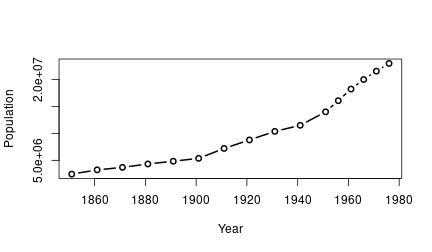
\includegraphics[width=\maxwidth]{FIGS/matrix-methods-plot-old-Canada-census-data-1} 
\end{knitrout}
\end{frame}


\begin{frame}[fragile]
But wait, this is only to 1976..! Looking around, we find another table here. There's a download csv link in there, let us see where this leads us. The table is 720KB, so surely there must be more to this than just the population. To get a sense of that, we dump the whole data.frame, not just its head.

\begin{knitrout}
\definecolor{shadecolor}{rgb}{0.969, 0.969, 0.969}\color{fgcolor}\begin{kframe}
\begin{alltt}
\hldef{data_new} \hlkwb{=} \hlkwd{read.csv}\hldef{(}\hlsng{"https://www12.statcan.gc.ca/census-recensement/2011/dp-pd/vc-rv/download-telecharger/download-telecharger.cfm?Lang=eng&CTLG=98-315-XWE2011001&FMT=csv"}\hldef{)}
\hlkwd{head}\hldef{(data_new,} \hlnum{10}\hldef{)}
\end{alltt}
\begin{verbatim}
##    GEOGRAPHY.NAME            CHARACTERISTIC YEAR.S. TOTAL FLAG_TOTAL
## 1          Canada Population (in thousands)    1956 16081           
## 2          Canada Population (in thousands)    1961 18238           
## 3          Canada Population (in thousands)    1966 20015           
## 4          Canada Population (in thousands)    1971 21568           
## 5          Canada Population (in thousands)    1976 22993           
## 6          Canada Population (in thousands)    1981 24343           
## 7          Canada Population (in thousands)    1986 25309           
## 8          Canada Population (in thousands)    1991 27297           
## 9          Canada Population (in thousands)    1996 28847           
## 10         Canada Population (in thousands)    2001 30007
\end{verbatim}
\end{kframe}
\end{knitrout}
\end{frame}


\begin{frame}[fragile]
Haha, this looks quite nice but has way more information than we need: we just want the population of Canada and here we get 9960 rows. Also, the population of Canada is expressed in thousands, so once we selected what we want, we will need to multiply by 1,000.

There are many ways to select rows. Let us proceed as follows: we want the rows where the geography is "Canada" and the characteristic is "Population (in thousands)". Let us find those indices of rows that satisfy the first criterion, those that satisfy the second; if we then intersect these two sets of indices, we will have selected the rows we want.

\begin{knitrout}
\definecolor{shadecolor}{rgb}{0.969, 0.969, 0.969}\color{fgcolor}\begin{kframe}
\begin{alltt}
\hldef{idx_CAN} \hlkwb{=} \hlkwd{which}\hldef{(data_new}\hlopt{$}\hldef{GEOGRAPHY.NAME} \hlopt{==} \hlsng{"Canada"}\hldef{)}
\hldef{idx_char} \hlkwb{=} \hlkwd{which}\hldef{(data_new}\hlopt{$}\hldef{CHARACTERISTIC} \hlopt{==} \hlsng{"Population (in thousands)"}\hldef{)}
\hldef{idx_keep} \hlkwb{=} \hlkwd{intersect}\hldef{(idx_CAN, idx_char)}
\hlkwd{head}\hldef{(idx_keep,} \hlkwc{n} \hldef{=} \hlnum{8}\hldef{)}
\end{alltt}
\begin{verbatim}
## [1] 1 2 3 4 5 6 7 8
\end{verbatim}
\end{kframe}
\end{knitrout}
\end{frame}


\begin{frame}[fragile]
Yes, this looks okay, so let us keep only these

\begin{knitrout}
\definecolor{shadecolor}{rgb}{0.969, 0.969, 0.969}\color{fgcolor}\begin{kframe}
\begin{alltt}
\hldef{data_new} \hlkwb{=} \hldef{data_new[idx_keep,]}
\hlkwd{head}\hldef{(data_new,} \hlkwc{n} \hldef{=} \hlnum{8}\hldef{)}
\end{alltt}
\begin{verbatim}
##   GEOGRAPHY.NAME            CHARACTERISTIC YEAR.S. TOTAL FLAG_TOTAL
## 1         Canada Population (in thousands)    1956 16081           
## 2         Canada Population (in thousands)    1961 18238           
## 3         Canada Population (in thousands)    1966 20015           
## 4         Canada Population (in thousands)    1971 21568           
## 5         Canada Population (in thousands)    1976 22993           
## 6         Canada Population (in thousands)    1981 24343           
## 7         Canada Population (in thousands)    1986 25309           
## 8         Canada Population (in thousands)    1991 27297
\end{verbatim}
\end{kframe}
\end{knitrout}
\end{frame}


\begin{frame}
We want to concatenate this data.frame with the one from earlier
\vfill
To do this, we need the two data frames to have the same number of columns and, actually, the same column names and entry types (notice that \code{YEAR.S.} in \code{data\_new} is a column of characters)
\end{frame}

\begin{frame}\frametitle{What remains to do}
\begin{itemize}
\item Rename the columns in the pruned old data (data\_pruned) to \code{year} and \code{population}. Personally, I prefer lowercase column names.. and \code{population} is more informative than \code{Canada}
\item Keep only the relevant columns in \code{data\_new}, rename them accordingly and multiply population by 1,000 there
\item Transform year in \code{data\_new} to numbers
\item We already have data up to and including 1976 in \code{data\_old}, so get rid of that in \code{data\_new}
\item Append the rows of \code{data\_new} to those of \code{data\_pruned}
\end{itemize}
\end{frame}


\begin{frame}[fragile]
\begin{knitrout}
\definecolor{shadecolor}{rgb}{0.969, 0.969, 0.969}\color{fgcolor}\begin{kframe}
\begin{alltt}
\hlkwd{colnames}\hldef{(data_old)} \hlkwb{=} \hlkwd{c}\hldef{(}\hlsng{"year"}\hldef{,} \hlsng{"population"}\hldef{)}
\hldef{data_new} \hlkwb{=} \hldef{data_new[,}\hlkwd{c}\hldef{(}\hlsng{"YEAR.S."}\hldef{,}\hlsng{"TOTAL"}\hldef{)]}
\hlkwd{colnames}\hldef{(data_new)} \hlkwb{=} \hlkwd{c}\hldef{(}\hlsng{"year"}\hldef{,} \hlsng{"population"}\hldef{)}
\hldef{data_new}\hlopt{$}\hldef{year} \hlkwb{=} \hlkwd{as.numeric}\hldef{(data_new}\hlopt{$}\hldef{year)}
\hldef{data_new} \hlkwb{=} \hldef{data_new[}\hlkwd{which}\hldef{(data_new}\hlopt{$}\hldef{year}\hlopt{>}\hlnum{1976}\hldef{),]}
\hldef{data_new}\hlopt{$}\hldef{population} \hlkwb{=} \hldef{data_new}\hlopt{$}\hldef{population}\hlopt{*}\hlnum{1000}

\hldef{data} \hlkwb{=} \hlkwd{rbind}\hldef{(data_old,data_new)}
\end{alltt}
\end{kframe}
\end{knitrout}
\end{frame}


\begin{frame}[fragile]\frametitle{Let us plot the result}
\begin{knitrout}
\definecolor{shadecolor}{rgb}{0.969, 0.969, 0.969}\color{fgcolor}\begin{kframe}
\begin{alltt}
\hlkwd{plot}\hldef{(data}\hlopt{$}\hldef{year, data}\hlopt{$}\hldef{population,}
    \hlkwc{type} \hldef{=} \hlsng{"b"}\hldef{,} \hlkwc{lwd} \hldef{=} \hlnum{2}\hldef{,}
    \hlkwc{xlab} \hldef{=} \hlsng{"Year"}\hldef{,} \hlkwc{ylab} \hldef{=} \hlsng{"Population"}\hldef{)}
\end{alltt}
\end{kframe}
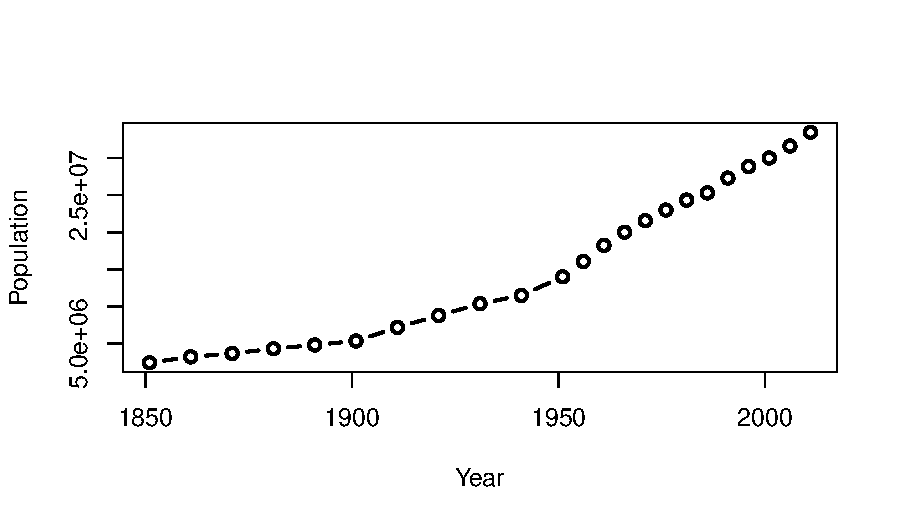
\includegraphics[width=\maxwidth]{FIGS/matrix-methods-plot-whole-Canada-census-data-1} 
\end{knitrout}
\end{frame}

\begin{frame}[fragile]\frametitle{Save the processed data}
In case we need the data elsewhere, we save the data to a \code{csv} file
\vfill
\begin{knitrout}
\definecolor{shadecolor}{rgb}{0.969, 0.969, 0.969}\color{fgcolor}\begin{kframe}
\begin{alltt}
\hlkwd{write.csv}\hldef{(data,} \hlkwc{file} \hldef{=} \hlsng{"../CODE/Canada_census.csv"}\hldef{)}
\end{alltt}
\end{kframe}
\end{knitrout}
\vfill
Using \code{readr} saves the data without row numbers (by default), so we can do this instead
\vfill
\begin{knitrout}
\definecolor{shadecolor}{rgb}{0.969, 0.969, 0.969}\color{fgcolor}\begin{kframe}
\begin{alltt}
\hldef{readr}\hlopt{::}\hlkwd{write_csv}\hldef{(data,} \hlkwc{file} \hldef{=} \hlsng{"../CODE/Canada_census.csv"}\hldef{)}
\end{alltt}
\end{kframe}
\end{knitrout}
\end{frame}

%%%%%%%%%%%%%%%%%%%%%
%%%%%%%%%%%%%%%%%%%%%
\subsection{Least squares problem -- Initial considerations}
\newSubSectionSlide{FIGS/Gemini_Generated_Image_gc7vxngc7vxngc7v.jpeg}

\begin{frame}
We just collected the census data for Canada
\vfill
Suppose we want to predict the population of Canada in 20 years given the historical population growth seen in the previous plot. What can we do?
\vfill
If there were just two points, we could easily "drive" a line through these two points. However, we have much more than two points, so we will use \emph{fitting}, \emph{i.e.}, try to make a curve come as close to possible to the points
\vfill
We start with a line, giving rise to \defword{linear least squares}
\end{frame}

\begin{frame}[fragile]\frametitle{Least squares approximation -- A trivial case}
\begin{knitrout}
\definecolor{shadecolor}{rgb}{0.969, 0.969, 0.969}\color{fgcolor}
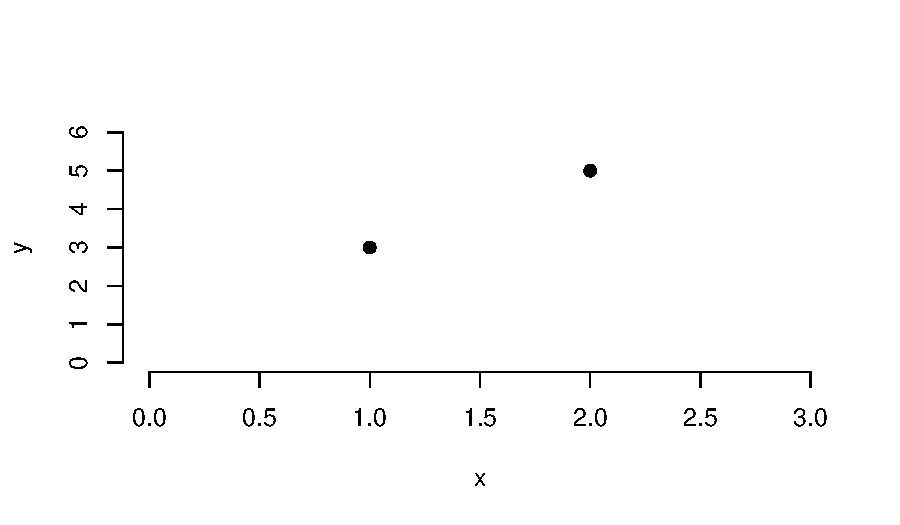
\includegraphics[width=\maxwidth]{FIGS/matrix-methods-plot-2-points-and-line-1} 
\end{knitrout}
\end{frame}

\begin{frame}
We want to find the equation of a line $y=a+bx$ that goes through these two points, i.e., we seek $a$ and $b$ such that
$$
\begin{aligned}
3 &= a+b \\
5 &= a+2b
\end{aligned}
$$
i.e., they satisfy $y=a+bx$ for $(x,y)=(1,3)$ and $(x,y)=(2,5)$
\end{frame}

\begin{frame}
This is a linear system with 2 equations and 2 unknowns $a$ and $b$
$$
\begin{pmatrix}
1 & 1 \\ 1 & 2
\end{pmatrix}
\begin{pmatrix}
a \\ b
\end{pmatrix}
=
\begin{pmatrix}
3 \\ 5
\end{pmatrix}
$$
\end{frame}

\begin{frame}[fragile]
We know from the ``famous'' linear algebra in a nutshell theorem that this system has a unique solution if the matrix
$$
M=
\begin{pmatrix}
1 & 1 \\ 1 & 2
\end{pmatrix}
$$
is invertible
\vfill
$\det(M)=1$, so we are good, we'll find $a$ and $b$ easily..
\end{frame}

\begin{frame}[fragile]
Now let's add another point
\begin{knitrout}
\definecolor{shadecolor}{rgb}{0.969, 0.969, 0.969}\color{fgcolor}\begin{kframe}
\begin{alltt}
\hldef{points} \hlkwb{=} \hlkwd{list}\hldef{()}
\hldef{points}\hlopt{$}\hldef{x} \hlkwb{=} \hlkwd{c}\hldef{(}\hlnum{1}\hldef{,}\hlnum{2}\hldef{,}\hlnum{3}\hldef{)}
\hldef{points}\hlopt{$}\hldef{y} \hlkwb{=} \hlkwd{c}\hldef{(}\hlnum{3}\hldef{,}\hlnum{5}\hldef{,}\hlnum{4}\hldef{)} \hlcom{# So the points are (1,3), (2,5) and (3,4)}
\hlkwd{plot}\hldef{(points}\hlopt{$}\hldef{x, points}\hlopt{$}\hldef{y,}
     \hlkwc{pch} \hldef{=} \hlnum{19}\hldef{,} \hlkwc{cex} \hldef{=} \hlnum{2}\hldef{,} \hlkwc{bty} \hldef{=} \hlsng{"n"}\hldef{,}
    \hlkwc{xlim} \hldef{=} \hlkwd{c}\hldef{(}\hlnum{0}\hldef{,} \hlnum{3.5}\hldef{),} \hlkwc{ylim} \hldef{=} \hlkwd{c}\hldef{(}\hlnum{0}\hldef{,}\hlnum{6}\hldef{),} \hlkwc{xlab} \hldef{=} \hlsng{"x"}\hldef{,} \hlkwc{ylab} \hldef{=} \hlsng{"y"}\hldef{)}
\end{alltt}
\end{kframe}
\end{knitrout}
These points are clearly not colinear, so there is not one line going through the 3
\end{frame}

\begin{frame}
We end up with an *overdetermined* system
$$
\begin{aligned}
3 &= a+b \\
5 &= a+2b \\
4 &= a+3b
\end{aligned}
$$
i.e.,
$$
\begin{pmatrix}
1 & 1 \\ 1 & 2 \\ 1 & 3
\end{pmatrix}
\begin{pmatrix}
a \\ b
\end{pmatrix}
=
\begin{pmatrix}
3 \\ 5 \\ 4
\end{pmatrix}
$$
\end{frame}

\begin{frame}[fragile]
We have verified visually that the points are not colinear, so this system has no solution.

(If you had to do it for good, you consider two vectors stemming from these 3 points and compute the angle between them or check that one is a multiple of the other).

So let us instead try to find the line that comes "closest" to the 3 points.

\begin{knitrout}
\definecolor{shadecolor}{rgb}{0.969, 0.969, 0.969}\color{fgcolor}\begin{kframe}
\begin{alltt}
\hldef{A} \hlkwb{=} \hlkwd{matrix}\hldef{(}\hlkwd{c}\hldef{(}\hlnum{1}\hldef{,}\hlnum{1}\hldef{,}\hlnum{1}\hldef{,}\hlnum{2}\hldef{),} \hlkwc{nr} \hldef{=} \hlnum{2}\hldef{,} \hlkwc{nc} \hldef{=} \hlnum{2}\hldef{,} \hlkwc{byrow} \hldef{=} \hlnum{TRUE}\hldef{)}
\hldef{rhs} \hlkwb{=} \hlkwd{matrix}\hldef{(}\hlkwd{c}\hldef{(}\hlnum{3}\hldef{,}\hlnum{5}\hldef{),} \hlkwc{nr} \hldef{=} \hlnum{2}\hldef{,} \hlkwc{nc} \hldef{=}\hlnum{1}\hldef{)}
\hldef{coefs} \hlkwb{=} \hlkwd{solve}\hldef{(A,rhs)} \hlcom{# To invert A, in R, you use solve(A), to solve Ax=b, you use solve(A,b)}
\hlkwd{plot}\hldef{(points}\hlopt{$}\hldef{x, points}\hlopt{$}\hldef{y,}
     \hlkwc{pch} \hldef{=} \hlnum{19}\hldef{,} \hlkwc{cex} \hldef{=} \hlnum{2}\hldef{,} \hlkwc{bty} \hldef{=} \hlsng{"n"}\hldef{,}
    \hlkwc{xlim} \hldef{=} \hlkwd{c}\hldef{(}\hlnum{0}\hldef{,} \hlnum{3.5}\hldef{),} \hlkwc{ylim} \hldef{=} \hlkwd{c}\hldef{(}\hlnum{0}\hldef{,}\hlnum{6}\hldef{),} \hlkwc{xlab} \hldef{=} \hlsng{"x"}\hldef{,} \hlkwc{ylab} \hldef{=} \hlsng{"y"}\hldef{)}
\hlkwd{abline}\hldef{(}\hlkwc{coef} \hldef{= coefs,} \hlkwc{lwd} \hldef{=} \hlnum{2}\hldef{)}
\end{alltt}
\end{kframe}
\end{knitrout}

Obviously, not sensational..
\end{frame}

\begin{frame}[fragile]
\begin{knitrout}
\definecolor{shadecolor}{rgb}{0.969, 0.969, 0.969}\color{fgcolor}\begin{kframe}
\begin{alltt}
\hlkwd{plot}\hldef{(points}\hlopt{$}\hldef{x, points}\hlopt{$}\hldef{y,}
     \hlkwc{pch} \hldef{=} \hlnum{19}\hldef{,} \hlkwc{cex} \hldef{=} \hlnum{2}\hldef{,} \hlkwc{bty} \hldef{=} \hlsng{"n"}\hldef{,}
    \hlkwc{xlim} \hldef{=} \hlkwd{c}\hldef{(}\hlnum{0}\hldef{,} \hlnum{3.5}\hldef{),} \hlkwc{ylim} \hldef{=} \hlkwd{c}\hldef{(}\hlnum{0}\hldef{,}\hlnum{6}\hldef{),} \hlkwc{xlab} \hldef{=} \hlsng{"x"}\hldef{,} \hlkwc{ylab} \hldef{=} \hlsng{"y"}\hldef{)}
\hlkwd{abline}\hldef{(}\hlkwc{coef} \hldef{= coefs,} \hlkwc{lwd} \hldef{=} \hlnum{2}\hldef{)}
\hlkwd{abline}\hldef{(}\hlkwc{a} \hldef{=} \hlnum{3}\hldef{,} \hlkwc{b} \hldef{=} \hlnum{0.5}\hldef{,} \hlkwc{lwd} \hldef{=} \hlnum{2}\hldef{,} \hlkwc{col} \hldef{=} \hlsng{"red"}\hldef{)}
\end{alltt}
\end{kframe}
\end{knitrout}

How do we find "how far away"?

- We could use projections onto the line (which we know minimises the distance)
- However, this will be a problem if we later decide that rather than a straight line, we want to use something more "funky" like a quadratic or an exponential
\end{frame}


\begin{frame}
So instead, we compare, for a given value $x$, the distance between the true value $y$ and the value of $y$ obtained using the curve (line, here) that we use to fit the data

Let $(x_i,y_i)$ be the data points, i.e., here, $(x_1,y_1)=(1,3)$, $(x_2,y_2)=(2,5)$ and $(x_3,y_3)=(3,4)$

Now suppose we use a line with equation $y=a+bx$ and that we pick a value for $a$ and $b$. Then at $x_1$,
$$
\tilde y_1 = a+bx_1 = a+b
$$
at $x_2$
$$
\tilde y_2 = a+bx_2 = a+2b
$$
and at $x_3$,
$$
\tilde y_3 = a+bx_3 = a+3b
$$
Consider $x_1$, for instance. The error we made by using the line with coefficients $(a,b)$ is $\overrightarrow{(x_1,y_1)(x_1,\tilde y_1)}$.
\end{frame}

\begin{frame}[fragile]
For future use, let us create a function for $y = a_0 + a_1x$.

\begin{knitrout}
\definecolor{shadecolor}{rgb}{0.969, 0.969, 0.969}\color{fgcolor}\begin{kframe}
\begin{alltt}
\hldef{my_line} \hlkwb{=} \hlkwa{function}\hldef{(}\hlkwc{x}\hldef{,} \hlkwc{a_0}\hldef{,} \hlkwc{a_1}\hldef{)\{}
    \hlkwd{return}\hldef{(a_0} \hlopt{+} \hldef{a_1}\hlopt{*}\hldef{x)}
\hldef{\}}
\end{alltt}
\end{kframe}
\end{knitrout}

Functions are super useful when programming

\begin{knitrout}
\definecolor{shadecolor}{rgb}{0.969, 0.969, 0.969}\color{fgcolor}\begin{kframe}
\begin{alltt}
\hlkwd{my_line}\hldef{(}\hlnum{1}\hldef{,}\hlnum{2}\hldef{,}\hlnum{3}\hldef{)}
\end{alltt}
\begin{verbatim}
## [1] 5
\end{verbatim}
\begin{alltt}
\hlkwd{my_line}\hldef{(}\hlkwc{a_0} \hldef{=} \hlnum{2}\hldef{,} \hlkwc{a_1} \hldef{=} \hlnum{3}\hldef{,} \hlkwc{x} \hldef{=} \hlnum{1}\hldef{)}
\end{alltt}
\begin{verbatim}
## [1] 5
\end{verbatim}
\begin{alltt}
\hlkwd{my_line}\hldef{(}\hlkwc{x} \hldef{=} \hlkwd{c}\hldef{(}\hlnum{1}\hldef{,}\hlnum{2}\hldef{,}\hlnum{3}\hldef{),} \hlkwc{a_0} \hldef{=} \hlnum{2}\hldef{,} \hlkwc{a_1} \hldef{=} \hlnum{3}\hldef{)}
\end{alltt}
\begin{verbatim}
## [1]  5  8 11
\end{verbatim}
\end{kframe}
\end{knitrout}
\end{frame}


\begin{frame}[fragile]
\begin{knitrout}
\definecolor{shadecolor}{rgb}{0.969, 0.969, 0.969}\color{fgcolor}\begin{kframe}
\begin{alltt}
\hldef{a} \hlkwb{=} \hlnum{3}
\hldef{b} \hlkwb{=} \hlnum{0.5} \hlcom{# The line has equation y=a+bx}
\hlkwd{plot}\hldef{(points}\hlopt{$}\hldef{x, points}\hlopt{$}\hldef{y,}
     \hlkwc{pch} \hldef{=} \hlnum{19}\hldef{,} \hlkwc{cex} \hldef{=} \hlnum{2}\hldef{,} \hlkwc{bty} \hldef{=} \hlsng{"n"}\hldef{,}
    \hlkwc{xlim} \hldef{=} \hlkwd{c}\hldef{(}\hlnum{0}\hldef{,} \hlnum{3.5}\hldef{),} \hlkwc{ylim} \hldef{=} \hlkwd{c}\hldef{(}\hlnum{0}\hldef{,}\hlnum{6}\hldef{),} \hlkwc{xlab} \hldef{=} \hlsng{"x"}\hldef{,} \hlkwc{ylab} \hldef{=} \hlsng{"y"}\hldef{)}
\hlkwd{abline}\hldef{(}\hlkwc{a} \hldef{= a,} \hlkwc{b} \hldef{= b,} \hlkwc{lwd} \hldef{=} \hlnum{2}\hldef{)}
\hlkwd{abline}\hldef{(}\hlkwc{v} \hldef{=} \hlkwd{c}\hldef{(}\hlnum{1}\hldef{,}\hlnum{2}\hldef{,}\hlnum{3}\hldef{))}  \hlcom{# If we used abline(h=c(0,1)), we would get horizontal lines at y=0 and y=1}
\hldef{p} \hlkwb{=} \hlkwd{my_line}\hldef{(}\hlkwd{c}\hldef{(}\hlnum{1}\hldef{,}\hlnum{2}\hldef{,}\hlnum{3}\hldef{), a, b)}
\hlkwd{points}\hldef{(}\hlkwd{c}\hldef{(}\hlnum{1}\hldef{,}\hlnum{2}\hldef{,}\hlnum{3}\hldef{), p,} \hlkwc{pch} \hldef{=} \hlnum{19}\hldef{,} \hlkwc{cex} \hldef{=} \hlnum{2}\hldef{,} \hlkwc{col} \hldef{=} \hlsng{"red"}\hldef{)}
\end{alltt}
\end{kframe}
\end{knitrout}
\end{frame}

\begin{frame}
Let us return to the error
$$
\overrightarrow{(x_1,y_1)(x_1,\tilde y_1)}
$$
We have
$$
\overrightarrow{(x_1,y_1)(x_1,\tilde y_1)}
= (x_1-x_1,y_1-\tilde y_1)
= (0, y_1-\tilde y_1)
$$
Let us call
$$
\varepsilon_1 = y_1-\tilde y_1
$$
We can compute $\varepsilon_2$ and $\varepsilon_3$ too. And we can then form the **error vector**
$$
\mathbf{e} = (\varepsilon_1,\varepsilon_2,\varepsilon_3)^T
$$
The norm of $\mathbf{e}$, $\|\mathbf{e}\|$, then tells us how much error we are making for the choice of $(a,b)$ we are using
\end{frame}


\begin{frame}
The norm of $\mathbf{e}$, $\|\mathbf{e}\|$, tells us how much error we are making for the choice of $(a,b)$ we are using

So our objective is to find $(a,b)$ such that $\|\mathbf{e}\|$ is minimal

We could use various norms, but the Euclidean norm has some very interesting properties, so we use
$$
\|\mathbf{e}\| = \sqrt{\varepsilon_1^2+\varepsilon_2^2+\varepsilon_3^2}
$$
\end{frame}


\begin{frame}\frametitle{The linear least squares problem}
Given a collection of data points $(x_1,y_1),\ldots,(x_n,y_n)$, find the coefficients $a,b$ of the line $y=a+bx$ such that
$$
\|\mathbf{e}\|=\sqrt{\varepsilon_1^2+\cdots+\varepsilon_n^2}
=\sqrt{(y_1-\tilde y_1)^2+\cdots+(y_n-\tilde y_n)^2}
$$
is minimal, where $\tilde y_i=a+bx_i$, for $i=1,\ldots,n$
\end{frame}


\begin{frame}[fragile]
Let us first hack a brute force solution! (For the example we have been using this far)

We have our three points in the list `points`, the function \code{my\_line} that computes the value $\tilde y$ given $x$ and $a,b$, so let us make a new function that, given $a,b$, computes $\mathbf{e}$

We'll also pass the points `points`

\begin{knitrout}
\definecolor{shadecolor}{rgb}{0.969, 0.969, 0.969}\color{fgcolor}\begin{kframe}
\begin{alltt}
\hldef{error} \hlkwb{=} \hlkwa{function}\hldef{(}\hlkwc{a_0}\hldef{,} \hlkwc{a_1}\hldef{,} \hlkwc{points}\hldef{) \{}
    \hldef{y_tilde} \hlkwb{=} \hlkwd{my_line}\hldef{(points}\hlopt{$}\hldef{x,} \hlkwc{a_0} \hldef{= a_0,} \hlkwc{a_1} \hldef{= a_1)}
    \hldef{e} \hlkwb{=} \hldef{points}\hlopt{$}\hldef{y} \hlopt{-} \hldef{y_tilde}
    \hlkwd{return}\hldef{(}\hlkwd{sqrt}\hldef{(}\hlkwd{sum}\hldef{(e}\hlopt{^}\hlnum{2}\hldef{)))}
\hldef{\}}
\hlkwd{error}\hldef{(}\hlkwc{a_0} \hldef{=} \hlnum{2}\hldef{,} \hlkwc{a_1} \hldef{=} \hlnum{3}\hldef{, points)}
\end{alltt}
\begin{verbatim}
## [1] 7.874008
\end{verbatim}
\begin{alltt}
\hlkwd{error}\hldef{(}\hlkwc{a_0} \hldef{=} \hlnum{3}\hldef{,} \hlkwc{a_1} \hldef{=} \hlnum{0.5}\hldef{, points)}
\end{alltt}
\begin{verbatim}
## [1] 1.224745
\end{verbatim}
\begin{alltt}
\hlkwd{error}\hldef{(}\hlkwc{a_0} \hldef{=} \hlnum{3.1}\hldef{,} \hlkwc{a_1} \hldef{=} \hlnum{0.48}\hldef{, points)}
\end{alltt}
\begin{verbatim}
## [1] 1.229471
\end{verbatim}
\end{kframe}
\end{knitrout}

We can't be doing this by hand..
\end{frame}


\begin{frame}\frametitle{Genetic algorithms}
Let's use something cool: a \emph{genetic algorithm}

- Genetic algorithms are a stochastic *optimisation* method. There are other types, e.g., gradient descent (deterministic)
- The idea is to use a mechanism mimicking evolution's drive towards higher fitness
- The function value is its fitness
- We try different genes (here, different values of $a,b$) and evaluate their fitness.. keep the good ones
- We mutate or crossover genes, throw in new ones, etc.
- We keep doing this until we reach a stopping criterion
- We then return the best gene we found
\end{frame}


\begin{frame}[fragile]
\begin{knitrout}
\definecolor{shadecolor}{rgb}{0.969, 0.969, 0.969}\color{fgcolor}\begin{kframe}
\begin{alltt}
\hlkwa{if} \hldef{(}\hlopt{!}\hlkwd{require}\hldef{(}\hlsng{"GA"}\hldef{,} \hlkwc{quietly} \hldef{=} \hlnum{TRUE}\hldef{)) \{}
  \hlkwd{install.packages}\hldef{(}\hlsng{"GA"}\hldef{)}
  \hlkwd{library}\hldef{(GA)}
\hldef{\}}
\hldef{GA} \hlkwb{=} \hlkwd{ga}\hldef{(}\hlkwc{type} \hldef{=} \hlsng{"real-valued"}\hldef{,}
        \hlkwc{fitness} \hldef{=} \hlkwa{function}\hldef{(}\hlkwc{x}\hldef{)} \hlopt{-}\hlkwd{error}\hldef{(}\hlkwc{a_0} \hldef{= x[}\hlnum{1}\hldef{],} \hlkwc{a_1} \hldef{= x[}\hlnum{2}\hldef{], points),}
        \hlkwc{suggestions} \hldef{=} \hlkwd{c}\hldef{(}\hlkwc{a_0} \hldef{=} \hlnum{2}\hldef{,} \hlkwc{a_1} \hldef{=} \hlnum{3}\hldef{),}
        \hlkwc{lower} \hldef{=} \hlkwd{c}\hldef{(}\hlopt{-}\hlnum{10}\hldef{,} \hlopt{-}\hlnum{10}\hldef{),} \hlkwc{upper} \hldef{=} \hlkwd{c}\hldef{(}\hlnum{10}\hldef{,} \hlnum{10}\hldef{),}
        \hlkwc{popSize} \hldef{=} \hlnum{200}\hldef{,} \hlkwc{maxiter} \hldef{=} \hlnum{150}\hldef{)}
\hlcom{# plot(GA)}
\hldef{GA}
\end{alltt}
\begin{verbatim}
## An object of class "ga"
## 
## Call:
## ga(type = "real-valued", fitness = function(x) -error(a_0 = x[1],     a_1 = x[2], points), lower = c(-10, -10), upper = c(10, 10),     popSize = 200, maxiter = 150, suggestions = c(a_0 = 2, a_1 = 3))
## 
## Available slots:
##  [1] "call"         "type"         "lower"        "upper"        "nBits"       
##  [6] "names"        "popSize"      "iter"         "run"          "maxiter"     
## [11] "suggestions"  "population"   "elitism"      "pcrossover"   "pmutation"   
## [16] "optim"        "fitness"      "summary"      "bestSol"      "fitnessValue"
## [21] "solution"
\end{verbatim}
\begin{alltt}
\hldef{GA}\hlopt{@}\hlkwc{solution}
\end{alltt}
\begin{verbatim}
##            x1       x2
## [1,] 2.999678 0.500084
\end{verbatim}
\begin{alltt}
\hlopt{-}\hldef{GA}\hlopt{@}\hlkwc{fitnessValue}
\end{alltt}
\begin{verbatim}
## [1] 1.224745
\end{verbatim}
\end{kframe}
\end{knitrout}

- Here, however, we do not have to go brute force: we can reason using mathematics
- We now take a little detour on the math side of things, we will come back to code in a while..
\end{frame}



%%%%%%%%%%%%%%%%%%%%%
%%%%%%%%%%%%%%%%%%%%%
\subsection{Least squares problem}
\newSubSectionSlide{FIGS/Gemini_Generated_Image_skqdtfskqdtfskqd.jpeg}

\begin{frame}{The least squares problem (simplest version)}
	\begin{definition}
		Given a collection of points $(x_1,y_1),\ldots,(x_n,y_n)$, find the coefficients $a,b$ of the line $y=a+bx$ such that
		$$
		\|\mathbf{e}\|=\sqrt{\varepsilon_1^2+\cdots+\varepsilon_n^2}
		=\sqrt{(y_1-\tilde y_1)^2+\cdots+(y_n-\tilde y_n)^2}
		$$
		is minimal, where $\tilde y_i=a+bx_i$ for $i=1,\ldots,n$
	\end{definition}
	\vfill
	We just saw how to solve this by brute force using a genetic algorith to minimise $\|e\|$, let us now see how to solve this problem ``properly''
\end{frame}


\begin{frame}
	For a data point $i=1,\ldots,n$
	\[
	\varepsilon_i = y_i-\tilde y_i = y_i - (a+bx_i)
	\]
	So if we write this for all data points,
	\begin{align*}
	\varepsilon_1 &= y_1 - (a+bx_1) \\
	&\;\;\vdots \\
	\varepsilon_n &= y_n - (a+bx_n) \\
	\end{align*}
	In matrix form
	\[
	\be = \bb-A\bx
	\]
	with
	\[
	\be = \begin{pmatrix}
	\varepsilon_1\\ \vdots\\ \varepsilon_n
	\end{pmatrix},
	A=\begin{pmatrix}
	1 & x_1 \\ \vdots & \vdots \\ 1 & x_n
	\end{pmatrix},
	\bx = \begin{pmatrix}
	a\\b
	\end{pmatrix}\textrm{ and }
	\bb = \begin{pmatrix}
	y_1\\ \vdots\\ y_n
	\end{pmatrix}
	\]
\end{frame}

\begin{frame}{The least squares problem (reformulated)}
\begin{definition}[Least squares solutions]
Consider a collection of points $(x_1,y_1),\ldots,(x_n,y_n)$, a matrix $A\in\M_{mn}$, $\bb\in\IR^m$. A \textbf{least squares solution} of $A\bx=\bb$ is a vector $\tilde \bx\in\IR^n$ s.t.
\[
\forall \bx\in\IR^n,\quad \|\bb-A\tilde\bx\|\leq \|\bb-A\bx\|
\]
\end{definition}
\end{frame}


\begin{frame}{Needed to solve the problem}
\begin{definition}[Best approximation]
Let $V$ be a vector space, $W\subset V$ and $\mathbf{v}\in V$. The \textbf{best approximation} to $\mathbf{v}$ in $W$ is $\tilde{\mathbf{v}}\in W$ s.t.
\[
\forall\mathbf{w}\in W, \mathbf{w}\neq\tilde{\mathbf{v}}, \quad
\|\mathbf{v}-\tilde{\mathbf{v}}\| < \|\mathbf{v}-\mathbf{w}\|
\]
\end{definition}
\vfill
\begin{theorem}[Best approximation theorem]
Let $V$ be a vector space with an inner product, $W\subset V$ and $\mathbf{v}\in V$. Then $\mathsf{proj}_W(\mathbf{v})$ is the best approximation to $\mathbf{v}$ in W
\end{theorem}
\end{frame}


\begin{frame}{Let us find the least squares solution}
$\forall \bx\IR^n$, $A\bx$ is a vector in the \textbf{column space} of $A$ (the space spanned by the vectors making up the columns of $A$)
\vfill
Since $\bx\in\IR^n$, $A\bx\in\mathsf{col}(A)$
\vfill
$\implies$ least squares solution of $A\bx=\bb$ is a vector $\tilde\by\in\mathsf{col}(A)$ s.t.
\[
\forall\by\in\mathsf{col}(A),\quad\|\bb-\tilde\by\|\leq\|\bb-\by\|
\]
\vfill
This looks very much like Best approximation and Best approximation theorem
\end{frame}

\begin{frame}{Putting things together}
We just stated: The least squares solution of $A\bx=\bb$ is a vector $\tilde\by\in\mathsf{col}(A)$ s.t.
\[
\forall\by\in\mathsf{col}(A),\quad\|\bb-\tilde\by\|\leq\|\bb-\by\|
\]
\vfill
We know (reformulating a tad):
\begin{theorem}[Best approximation theorem]
Let $V$ be a vector space with an inner product, $W\subset V$ and $\mathbf{v}\in V$. Then $\mathsf{proj}_W(\mathbf{v})\in W$ is the best approximation to $\mathbf{v}$ in W, i.e.,
\[
\forall\mathbf{w}\in W, \mathbf{w}\neq\mathsf{proj}_W(\mathbf{v}), \quad
\|\mathbf{v}-\mathsf{proj}_W(\mathbf{v})\| < \|\mathbf{v}-\mathbf{w}\|
\]
\end{theorem}
\vfill
$\implies$ $W=\mathsf{col}(A)$, $\bv=\bb$ and $\tilde\by=\mathsf{proj}_{\mathsf{col}(A)}(\mathbf{b})$
\end{frame}

\begin{frame}
So if $\tilde\bx$ is a least squares solution of $A\bx=\bb$, then
\[
\tilde\by = A\tilde\bx = \mathsf{proj}_{\mathsf{col}(A)}(\mathbf{b})
\]
\vfill
We have
\[
\bb-A\tilde\bx = \bb-\mathsf{proj}_{\mathsf{col}(A)}(\mathbf{b}) 
= \mathsf{perp}_{\mathsf{col}(A)}(\mathbf{b})
\]
and it is easy to show that
\[
\mathsf{perp}_{\mathsf{col}(A)}(\mathbf{b}) \perp \mathsf{col}(A)
\]
\vfill
So for all columns $\ba_i$ of $A$
\[
\ba_i\boldsymbol{\cdot}(\bb-A\tilde\bx) = 0
\]
which we can also write as $\ba_i^T(\bb-A\tilde\bx) = 0$
\end{frame}

\begin{frame}
For all columns $\ba_i$ of $A$,
\[\ba_i^T(\bb-A\tilde\bx) = 0
\]
\vfill
This is equivalent to saying that
\[
A^T(\bb-A\tilde\bx) = \b0
\]
\vfill
We have
\begin{align*}
A^T(\bb-A\tilde\bx) = \b0 &\iff A^T\bb - A^TA\tilde\bx = \b0 \\
&\iff A^T\bb = A^TA\tilde\bx \\
&\iff A^TA\tilde\bx = A^T\bb
\end{align*}
The latter system constitutes the \textbf{normal equations} for $\tilde\bx$
\end{frame}


\begin{frame}{Least squares theorem}
\begin{importanttheorem}[Least squares theorem]\label{th:least_squares}
$A\in\M_{mn}$, $\bb\in\IR^m$. Then
\begin{enumerate}
\item $A\bx=\bb$ always has at least one least squares solution $\tilde\bx$
\item $\tilde\bx$ least squares solution to $A\bx=\bb$ $\iff$ $\tilde\bx$ is a solution to the normal equations $A^TA\tilde\bx = A^T\bb$
\item $A$ has linearly independent columns $\iff$ $A^TA$ invertible.  
\newline In this case, the least squares solution is unique and 
\[
\tilde\bx = \left(A^TA\right)^{-1}A^T\bb
\]
\end{enumerate}
\end{importanttheorem}
\vfill
We have seen 1 and 2, we will not show 3 (it is not hard)
\end{frame}


%%%%%%%%%%%%%%%%%%%%%
%%%%%%%%%%%%%%%%%%%%%
\subsection{Fitting something more complicated}
\newSubSectionSlide{FIGS/Gemini_Generated_Image_jvdz0zjvdz0zjvdz.jpeg}

\begin{frame}{Suppose we want to fit something a bit more complicated..}
For instance, instead of the affine function
\[
y = a+bx
\]
suppose we want to do the quadratic
\[
y = a_0+a_1x+a_2x^2
\]
or even
\[
y = k_0 e^{k_1x}
\]
\vfill
How do we proceed?
\end{frame}


\begin{frame}{Fitting the quadratic}
We have the data points $(x_1,y_1),(x_2,y_2),\ldots,(x_n,y_n)$ and want to fit
\[
y = a_0+a_1x+a_2x^2
\]
At $(x_1,y_1)$,
\[
\tilde y_1 = a_0+a_1x_1+a_2x_1^2
\]
$\vdots$\\
At $(x_n,y_n)$,
\[
\tilde y_n = a_0+a_1x_n+a_2x_n^2
\]
\end{frame}

\begin{frame}
In terms of the error
\begin{align*}
\varepsilon_1 &= y_1-\tilde y_1 = y_1-(a_0+a_1x_1+a_2x_1^2) \\
&\;\;\vdots\\
\varepsilon_n &= y_n-\tilde y_n = y_n-(a_0+a_1x_n+a_2x_n^2)
\end{align*}
i.e.,
\[
\be = \bb-A\bx 
\]
where
\[
\be = \begin{pmatrix}
\varepsilon_1\\ \vdots\\ \varepsilon_n
\end{pmatrix},
A=\begin{pmatrix}
1 & x_1 & x_1^2\\ \vdots & \vdots & \vdots \\ 1 & x_n & x_n^2
\end{pmatrix},
\bx = \begin{pmatrix}
a_0\\a_1\\a_2
\end{pmatrix}\textrm{ and }
\bb = \begin{pmatrix}
y_1\\ \vdots\\ y_n
\end{pmatrix}
\]
\vfill
Theorem~\ref{th:least_squares} applies, with here $A\in\M_{n3}$ and $\bb\in\IR^n$
\end{frame}


\begin{frame}{Fitting the exponential}
Things are a bit more complicated here
\vfill
If we proceed as before, we get the system
\begin{align*}
y_1 &= k_0 e^{k_1x_1} \\
&\;\;\vdots \\
y_n &= k_0 e^{k_1x_n}
\end{align*}
$e^{k_1x_i}$ is a nonlinear term, it cannot be put in a matrix
\vfill
\emph{However}: take the $\ln$ of both sides of the equation
\[
\ln(y_i) = \ln(k_0e^{k_1x_i}) = \ln(k_0)+\ln(e^{k_1x_i}) = \ln(k_0)+k_1x_i
\]
If $y_i,k_0>0$, then their $\ln$ are defined and we're in business..
\end{frame}

\begin{frame}
\[
\ln(y_i) = \ln (k_0)+k_1x_i
\]
So the system is
\begin{align*}
\by = A\bx+\bb
\end{align*}
with
\[
A = \begin{pmatrix}
x_1\\ \vdots \\ x_n
\end{pmatrix},
\bx = \begin{pmatrix}
k_1
\end{pmatrix},
\bb = \begin{pmatrix}
\ln (k_0)
\end{pmatrix}
\textrm{ and }
\by = \begin{pmatrix}
\ln (y_1)\\ \vdots\\ \ln (y_n)
\end{pmatrix}
\]
\end{frame}




%%%%%%%%%%%%%%%%%%%%%
%%%%%%%%%%%%%%%%%%%%%
%%%%%%%%%%%%%%%%%%%%%
%%%%%%%%%%%%%%%%%%%%%
\section{QR factorisation}
\newSectionSlide{FIGS/Gemini_Generated_Image_c06eixc06eixc06e.jpeg}



%%%%%%%%%%%%%%%%%%%%%
%%%%%%%%%%%%%%%%%%%%%
\subsection{Matrix factorisations}
\newSubSectionSlide{FIGS/Gemini_Generated_Image_c06eixc06eixc06e.jpeg}
\begin{frame}{Matrix factorisations}
	Matrix factorisations are popular because they allow to perform some computations more easily
	\vfill
	There are several different types of factorisations. Here, we study just the QR factorisation, which is useful for many least squares problems
\end{frame}	
	

%%%%%%%%%%%%%%%%%%%%%
%%%%%%%%%%%%%%%%%%%%%
\subsection{Orthogonality and projections}
\newSubSectionSlide{FIGS/Gemini_Generated_Image_c06eixc06eixc06e.jpeg}

\begin{frame}
\begin{definition}[Orthogonal set of vectors]
The set of vectors $\{\bv_1,\ldots,\bv_k\}\in\IR^n$ is an \textbf{orthogonal set} if
\[
\forall i,j=1,\ldots,k,\quad i\neq j \implies \bv_i\bullet\bv_j=0
\]
\end{definition}

\begin{theorem}\label{th:ortho_implies_LI}
$\{\bv_1,\ldots,\bv_k\}\in\IR^n$ with $\forall i$, $\bv_i\neq\b0$, orthogonal set $\implies$ $\{\bv_1,\ldots,\bv_k\}\in\IR^n$ linearly independent
\end{theorem}

\begin{definition}[Orthogonal basis]
Let $S$ be a basis of the subspace $W\subset\IR^n$ composed of an orthogonal set of vectors. We say $S$ is an \textbf{orthogonal basis} of $W$
\end{definition}
\end{frame}

\begin{frame}{Proof of Theorem~\ref{th:ortho_implies_LI}}
Assume $\{\bv_1,\ldots,\bv_k\}$ orthogonal set with $\bv_i\neq\b0$ for all $i=1,\ldots,k$. Recall $\{\bv_1,\ldots,\bv_k\}$ is LI if 
\[
c_1\bv_1+\cdots+c_k\bv_k=\b0\iff c_1=\cdots=c_k=0
\]
So assume $c_1,\ldots,c_k\in\IR$ are s.t. $c_1\bv_1+\cdots+c_k\bv_k=\b0$.
Recall that $\forall\bx\in\IR^k$, $\b0_k\bullet\bx=0$. So for some $\bv_i\in\{\bv_1,\ldots,\bv_k\}$
\begin{align}
0 &= \b0\bullet\bv_i \nonumber \\
&= (c_1\bv_1+\cdots+c_k\bv_k)\bullet\bv_i \nonumber \\
&= c_1\bv_1\bullet\bv_i+\cdots+c_k\bv_k\bullet\bv_i \label{eq:proof_th_ortho_implies_LI}
\end{align}
As $\{\bv_1,\ldots,\bv_k\}$ orthogonal, $\bv_j\bullet\bv_i=0$ when $i\neq j$, \eqref{eq:proof_th_ortho_implies_LI} reduces to
\[
c_i\bv_i\bullet\bv_i = 0 \iff c_i\|\bv_i\|^2 = 0
\]
As $\bv_i\neq 0$ for all $i$, $\|\bv_i\|\neq 0$ and so $c_i=0$. This is true for all $i$, hence the result \hfill\qed
\end{frame}

\begin{frame}{Example -- Vectors of the standard basis of $\IR^3$}
For $\IR^3$, we denote
\[
\bi =\begin{pmatrix}
1\\0\\0
\end{pmatrix},\quad
\bj =\begin{pmatrix}
0\\1\\0
\end{pmatrix}
\textrm{ and }
\bk =\begin{pmatrix}
0\\0\\1
\end{pmatrix}
\]
($\IR^k$ for $k>3$, we denote them $\be_i$)
\vfill
Clearly, $\{\bi,\bj\}$, $\{\bi,\bk\}$, $\{\bj,\bk\}$ and $\{\bi,\bj,\bk\}$ orthogonal sets. The standard basis vectors are also $\neq\b0$, so the sets are LI. And
\[
\{\bi,\bj,\bk\}
\]
is an orthogonal basis of $\IR^3$ since it spans $\IR^3$ and is LI
\vfill
\[
c_1\bi+c_2\bj+c_3\bk
=
c_1\begin{pmatrix}
1\\0\\0
\end{pmatrix}
+c_2\begin{pmatrix}
0\\1\\0
\end{pmatrix}
+c_3\begin{pmatrix}
0\\0\\1
\end{pmatrix}
=
\begin{pmatrix}
c_1\\c_2\\c_3
\end{pmatrix}
\]
\end{frame}

\begin{frame}{Orthonormal version of things}
\begin{definition}[Orthonormal set]
The set of vectors $\{\bv_1,\ldots,\bv_k\}\in\IR^n$ is an \textbf{orthonormal set} if it is an orthogonal set and furthermore
\[
\forall i=1,\ldots,k,\quad \|\bv_i\|=1
\]
\end{definition}
\begin{definition}[Orthonormal basis]
A basis of the subspace $W\subset\IR^n$ is an \textbf{orthonormal basis} if the vectors composing it are an orthonormal set
\end{definition}
\vfill
$\{\bv_1,\ldots,\bv_k\}\in\IR^n$ is orthonormal if
\[
\bv_i\bullet\bv_j =
\begin{cases}
1 &\textrm{if }i=j \\
0 &\textrm{otherwise}
\end{cases}
\]
\end{frame}


\begin{frame}{Projections}
	\begin{definition}[Orthogonal projection onto a subspace]
	$W\subset\IR^n$ a subspace and $\{\bu_1,\ldots,\bu_k\}$ an orthogonal basis of $W$. $\forall\bv\in\IR^n$, the \textbf{orthogonal projection} of $\bv$ \textbf{onto} $W$ is
	\[
	\mathsf{proj}_W(\bv) =
	\frac{\bu_1\bullet\bv}{\|\bu_1\|^2}\bu_1
	+\cdots+
	\frac{\bu_k\bullet\bv}{\|\bu_k\|^2}\bu_k
	\]  
	\end{definition}
	\vfill
	\begin{definition}[Component orthogonal to a subspace]
	$W\subset\IR^n$ a subspace and $\{\bu_1,\ldots,\bu_k\}$ an orthogonal basis of $W$. $\forall\bv\in\IR^n$, the \textbf{component} of  $\bv$ \textbf{orthogonal to} W is
	\[
	\mathsf{perp}_W(\bv)=\bv-\mathsf{proj}_W(\bv)
	\]
	\end{definition}	
	\end{frame}
	
	
	\begin{frame}
	What this aims to do is to construct an orthogonal basis for a subspace $W\subset\IR^n$
	\vfill
	To do this, we use the \emph{Gram-Schmidt orthogonalisation process}, which turn s a basis of $W$ into an orthogonal basis of $W$
	\end{frame}
	
	\begin{frame}{Gram-Schmidt process}
	\begin{theorem}
	$W\subset\IR^n$ a subset and $\{\bx_1,\ldots,\bx_k\}$ a basis of $W$. Let
	\begin{align*}
	\bv_1 &= \bx_1 \\
	\bv_2 &= \bx_2 -\frac{\bv_1\bullet\bx_2}{\|\bv_1\|^2}\bv_1 \\
	\bv_3 &= \bx_3 -\frac{\bv_1\bullet\bx_3}{\|\bv_1\|^2}\bv_1 -\frac{\bv_2\bullet\bx_3}{\|\bv_2\|^2}\bv_2 \\
	&\;\;\vdots & \\
	\bv_k &= \bx_k -\frac{\bv_1\bullet\bx_k}{\|\bv_1\|^2}\bv_1 -\cdots-\frac{\bv_{k-1}\bullet\bx_k}{\|\bv_{k-1}\|^2}\bv_{k-1}
	\end{align*}
	and
	\[
	W_1=\mathsf{span}(\bx_1),W_2 = \mathsf{span}(\bx_1,\bx_2),\ldots,
	W_k = \mathsf{span}(\bx_1,\ldots,\bx_k)
	\]
	Then $\forall i=1,\ldots,k$, $\{\bv_1,\ldots,\bv_i\}$ orthogonal basis for $W_i$
	\end{theorem}
	\end{frame}
	
	


%%%%%%%%%%%%%%%%%%%%%
%%%%%%%%%%%%%%%%%%%%%
\subsection{Orthogonal matrices}
\newSubSectionSlide{FIGS/Gemini_Generated_Image_c06eixc06eixc06e.jpeg}

\begin{frame}
\begin{theorem}
Let $Q\in\M_{mn}$. The columns of $Q$ form an orthonormal set if and only if
\[
Q^TQ=\II_n
\]
\end{theorem}
\begin{definition}[Orthogonal matrix]
$Q\in\M_n$ is an \textbf{orthogonal matrix} if its columns form an orthonormal set 
\end{definition}
So $Q\in\M_n$ orthogonal if $Q^TQ=\II$, i.e., $Q^T=Q^{-1}$
\begin{theorem}[NSC for orthogonality]
$Q\in\M_n$ orthogonal $\iff$ $Q^{-1} = Q^T$
\end{theorem}
\end{frame}


\begin{frame}
\begin{theorem}[Orthogonal matrices ``encode" isometries]
\label{th:TFAE_orthogonal_matrices}
Let $Q\in\M_n$. TFAE
\begin{enumerate}
\item $Q$ orthogonal
\item $\forall\bx\in\IR^n$, $\|Q\bx\|=\|\bx\|$
\item $\forall\bx,\by\in\IR^n$, $Q\bx\bullet Q\by=\bx\bullet\by$
\end{enumerate}
\end{theorem}
\vfill
\begin{theorem}\label{th:properties_orthogonal_matrices}
Let $Q\in\M_n$ be orthogonal. Then
\begin{enumerate}
\item The rows of $Q$ form an orthonormal set
\item $Q^{-1}$ orthogonal
\item $\det Q=\pm 1$
\item $\forall\lambda\in\sigma(Q)$, $|\lambda|=1$
\item If $Q_2\in\M_n$ also orthogonal, then $QQ_2$ orthogonal
\end{enumerate}
\end{theorem}
\end{frame}



\begin{frame}{Proof of 4 in Theorem~\ref{th:properties_orthogonal_matrices}}
All statements in Theorem~\ref{th:properties_orthogonal_matrices} are easy, but let's focus on 4 
\vfill
Let $\lambda$ be an eigenvalue of $Q\in\M_n$ orthogonal, i.e., $\exists\IR^n\ni\bx\neq\b0$ s.t.
\[
Q\bx = \lambda\bx
\]
Take the norm on both sides
\[
\|Q\bx\| = \|\lambda\bx\|
\]
From 2 in Theorem~\ref{th:TFAE_orthogonal_matrices}, $\|Q\bx\|=\|\bx\|$ and from the properties of norms, $\|\lambda\bx\|=|\lambda|\;\|\bx\|$, so we have
\[
\|Q\bx\| = \|\lambda\bx\| \iff \|\bx\| = |\lambda|\;\|\bx\| \iff 1=|\lambda|
\]
(we can divide by $\|\bx\|$ since $\bx\neq \b0$ as an eigenvector)\hfill\qed
\end{frame}



%%%%%%%%%%%%%%%%%%%%%
%%%%%%%%%%%%%%%%%%%%%
\subsection{The QR factorisation}
\begin{frame}{The QR factorisation}
\begin{theorem}\label{th:QR_factorisation}
Let $A\in\M_{mn}$ with LI columns. Then $A$ can be factored as
\[
A=QR
\]
where $Q\in\M_{mn}$ has orthonormal columns and $R\in\M_n$ is nonsingular upper triangular
\end{theorem}
\end{frame}


\begin{frame}{Back to least squares}
So what was the point of all that..?
\vfill
\begin{theorem}[Least squares with QR factorisation]
\label{th:LSQ_with_QR}
$A\in\M_{mn}$ with LI columns, $\bb\in\IR^m$. If $A=QR$ is a QR factorisation of $A$, then the unique least squares solution $\tilde\bx$ of $A\bx=\bb$ is
\[
\tilde\bx = R^{-1}Q^T\bb
\]
\end{theorem}
\end{frame}


\begin{frame}{Proof of Theorem~\ref{th:LSQ_with_QR}}
$A$ has LI columns so 
\begin{itemize}
\item least squares $A\bx=\bb$ has unique solution $\tilde\bx=(A^TA)^{-1}A^T\bb$
\item by Theorem~\ref{th:QR_factorisation}, $A$ can be written as $A=QR$ with $Q\in\M_{mn}$ with orthonormal columns and $R\in\M_n$ nonsingular and upper triangular
\end{itemize}
So
\begin{align*}
A^TA\tilde\bx= A^T\bb &\implies (QR)^TQR\tilde\bx = (QR)^T\bb \\
&\implies R^TQ^TQR\tilde\bx = R^TQ^T\bb \\
&\implies R^T\II_nR\tilde\bx = R^TQ^T\bb \\
&\implies R^TR\tilde\bx = R^TQ^T\bb \\
&\implies (R^T)^{-1}R\tilde\bx = (R^T)^{-1}R^TQ^T\bb \\
&\implies R\tilde\bx = Q^T\bb \\
&\implies \tilde\bx = R^{-1}Q^T\bb\hfill\qed
\end{align*}
\end{frame}



%%%%%%%%%%%%%%%%%%%%%
%%%%%%%%%%%%%%%%%%%%%
%%%%%%%%%%%%%%%%%%%%%
%%%%%%%%%%%%%%%%%%%%%
\section{Singular values decomposition (SVD)}
\newSectionSlide{FIGS/Gemini_Generated_Image_c06eixc06eixc06e.jpeg}

\begin{frame}{Matrix factorisations (continued)}
The singular value decomposition (known mostly by its acronym, SVD) is yet another type of factorisation/decomposition..
\end{frame}

%%%%%%%%%%%%%%%%%%%%%
%%%%%%%%%%%%%%%%%%%%%
\subsection{Singular values}
\newSubSectionSlide{FIGS/Gemini_Generated_Image_c06eixc06eixc06e.jpeg}

\begin{frame}{Singular values}
\begin{definition}[Singular value]
Let $A\in\M_{mn}(\IR)$. The \textbf{singular values} of $A$ are the real numbers 
\[
\sigma_1\geq \sigma_2\geq\cdots\sigma_n\geq 0
\]
that are the square roots of the eigenvalues of $A^TA$
\end{definition}
\end{frame}


\begin{frame}{Singular values are real and nonnegative?}
Recall that $\forall A\in\M_{mn}$, $A^TA$ is symmetric
\vfill
\textbf{Claim 1.} Real symmetric matrices have real eigenvalues
\vfill
\textbf{Proof.} $A\in\M_n(\IR)$ symmetric and $(\lambda,\bv)$ eigenpair of $A$, i.e, $A\bv=\lambda\bv$. Taking the complex conjugate, $\overline{A\bv}=\overline{\lambda\bv}$
\vfill
Since $A\in\M_n(\IR)$, $\overline{A}=A$\qquad ($z=\bar z\iff z\in\IR$)
\vfill
So
\[
A\bar\bv=\overline{A}\bar\bv=\overline{A\bv}=\overline{\lambda\bv}=\overline{\lambda}\bar\bv
\]
i.e., if $(\lambda,\bv)$ eigenpair, $(\bar\lambda,\bar\bv)$ also eigenpair
\end{frame}

\begin{frame}
Still assuming $A\in\M_n(\IR)$ symmetric and $(\lambda,\bv)$ eigenpair of $A$ and using what we just proved (that $(\bar\lambda,\bar\bv)$ also eigenpair), take transposes
\begin{align*}
A\bar\bv = \bar\lambda\bar\bv &\iff (A\bar\bv)^T = (\bar\lambda\bar\bv)^T \\
&\iff \bar\bv^TA^T=\bar\lambda\bar\bv^T \\
&\iff \bar\bv^T A = \bar\lambda\bar\bv^T \qquad{\textrm{[$A$ symmetric]}}
\end{align*}
\vfill
Let us now compute $\lambda (\bar\bv\bullet\bv)$. We have
\begin{align*}
\lambda (\bar\bv\bullet\bv) &= \lambda\bar\bv^T\bv = \bar\bv^T(\lambda\bv) \\
&= \bar\bv^T(A\bv) = (\bar\bv^TA)\bv \\
&= (\bar\lambda\bar\bv^T)\bv = \bar\lambda(\bar\bv\bullet\bv) \\
&\iff (\lambda-\bar\lambda)(\bar\bv\bullet\bv) = 0
\end{align*}
\end{frame}

\begin{frame}
We have shown
\[
(\lambda-\bar\lambda)(\bar\bv\bullet\bv) = 0
\]
Let 
\[
\bv = \begin{pmatrix}
a_1+ib_1 \\
\vdots \\
a_n+ib_n
\end{pmatrix}
\]
Then
\[
\bar\bv = \begin{pmatrix}
a_1-ib_1 \\
\vdots \\
a_n-ib_n
\end{pmatrix}
\]
So
\[
\bar\bv\bullet\bv = (a_1^2+b_1^2)+\cdots+(a_n^2+b_n^2)
\]
But $\bv$ eigenvector is $\neq\b0$, so $\bar\bv\bullet\bv\neq 0$, so
\[
(\lambda-\bar\lambda)(\bar\bv\bullet\bv) = 0
\iff \lambda-\bar\lambda=0
\iff \lambda=\bar\lambda\iff \lambda\in\IR\qed
\]
\end{frame}


\begin{frame}
\textbf{Claim 2.} For $A\in\M_{mn}(\IR)$, the eigenvalues of $A^TA$ are real and nonnegative

\vfill
\textbf{Proof.}
We know that for $A\in\M_{mn}$, $A^TA$ symmetric and from previous claim, if $A\in\M_{mn}(\IR)$, then $A^TA$ is symmetric and real and with real eigenvalues
\vfill
Let $(\lambda,\bv)$ be an eigenpair of $A^TA$, with $\bv$ chosen so that $\|\bv\|=1$
\vfill 
Norms are functions $V\to\IR_+$, so $\|A\bv\|$ and $\|A\bv\|^2$ are $\geq 0$ and thus
\begin{align*}
0\leq \|A\bv\|^2 &= (A\bv)\bullet(A\bv) = (A\bv)^T(A\bv) \\
&= \bv^TA^TA\bv = \bv^T(A^TA\bv) = \bv^T(\lambda\bv) \\
&= \lambda(\bv^T\bv) = \lambda(\bv\bullet\bv) = \lambda\|\bv\|^2 \\
&= \lambda\hfill\qed
\end{align*}
\end{frame}

\begin{frame}
\textbf{Claim 3.} For $A\in\M_{mn}(\IR)$, the nonzero eigenvalues of $A^TA$ and $AA^T$ are the same
\vfill
\textbf{Proof.}
Let $(\lambda,\bv)$ be an eigenpair of $A^TA$ with $\lambda\neq 0$. Then $\bv\neq\b0$ and
\[
	A^TA\bv=\lambda\bv\neq\b0
\]
Left multiply by $A$
\[
	AA^TA\bv = \lambda A\bv
\]
Let $\bw=A\bv$, we thus have $AA^T\bw=\lambda\bw$; in other words, $A\bv$ is an eigenvector of $AA^T$ corresponding to the (nonzero) eigenvalue $\lambda$
\vfill
The reverse works the same way.. \qed
\end{frame}

%%%%%%%%%%%%%%%%%%%%%
%%%%%%%%%%%%%%%%%%%%%
\subsection{The SVD}
\newSubSectionSlide{FIGS/Gemini_Generated_Image_c06eixc06eixc06e.jpeg}

\begin{frame}{The singular value decomposition (SVD)}
\begin{importanttheorem}[SVD]\label{th:SVD}
$A\in\M_{mn}$ with singular values $\sigma_1\geq\cdots\geq\sigma_r>0$ and $\sigma_{r+1}=\cdots=\sigma_n=0$
\vskip0.5cm
Then there exists $U\in\M_m$ orthogonal, $V\in\M_n$ orthogonal and a block matrix $\Sigma\in\M_{mn}$ taking the form
\[
\Sigma=
\begin{pmatrix}
D & 0_{r,n-r} \\
0_{m-r,r} & 0_{m-r,n-r}
\end{pmatrix}
\]
where 
\[
D = \mathsf{diag}(\sigma_1,\ldots,\sigma_r)\in\M_r
\] 
such that
\[
A=U\Sigma V^T
\]
\end{importanttheorem}
\end{frame}


\begin{frame}
\begin{definition}
We call a factorisation as in Theorem~\ref{th:SVD} the \textbf{singular value decomposition} of $A$. The columns of $U$ and $V$ are, respectively, the \textbf{left} and \textbf{right singular vectors} of $A$
\end{definition}
\vfill
$U$ and $V^T$ are \emph{rotation} or \emph{reflection} matrices, $\Sigma$ is a \emph{scaling} matrix
\vfill
$U\in\M_m$ orthogonal matrix with columns the eigenvectors of $AA^T$
\vfill
$V\in\M_n$ orthogonal matrix with columns the eigenvectors of $A^TA$
\end{frame}


\begin{frame}{Outer product form of the SVD}
\begin{theorem}[Outer product form of the SVD]\label{th:SVD_outer_product_form}
$A\in\M_{mn}$ with singular values $\sigma_1\geq\cdots\geq\sigma_r>0$ and $\sigma_{r+1}=\cdots=\sigma_n=0$, $\bu_1,\ldots,\bu_r$ and $\bv_1,\ldots,\bv_r$, respectively, left and right singular vectors of $A$ corresponding to these singular values
\vskip0.5cm
Then 
\begin{equation}\label{eq:outer-product-form-SVD}
A=\sigma_1\bu_1\bv_1^T+\cdots+\sigma_r\bu_r\bv_r^T
\end{equation}
\end{theorem}
\end{frame}


\begin{frame}{Computing the SVD (case of $\neq$ eigenvalues)}
To compute the SVD, we use the following result
\vfill
\begin{theorem}\label{th:eigenvectors_of_symmetric_are_orthogonal}
Let $A\in\M_n$ symmetric, $(\lambda_1,\bu_1)$ and $(\lambda_2,\bu_2)$ be eigenpairs, $\lambda_1\neq\lambda_2$. Then $\bu_1\bullet\bu_2=0$
\end{theorem}
\end{frame}

\begin{frame}{Proof of Theorem~\ref{th:eigenvectors_of_symmetric_are_orthogonal}}
$A\in\M_n$ symmetric, $(\lambda_1,\bu_1)$ and $(\lambda_2,\bu_2)$ eigenpairs with $\lambda_1\neq\lambda_2$
\begin{align*}
\lambda_1(\bv_1\bullet\bv_2) 
&= (\lambda_1\bv_1)\bullet\bv_2 \\
&= A\bv_1\bullet\bv_2 \\
&= (A\bv_1)^T\bv_2 \\
&= \bv_1^TA^T\bv_2 \\
&= \bv_1^T(A\bv_2)  \qquad\textrm{[$A$ symmetric so $A^T=A$]} \\
&= \bv_1^T(\lambda_2\bv_2) \\
&= \lambda_2(\bv_1^T\bv_2) \\
&= \lambda_2(\bv_1\bullet\bv_2)
\end{align*}
\vfill
So $(\lambda_1-\lambda_2)(\bv_1\bullet\bv_2)=0$. But $\lambda_1\neq\lambda_2$, so $\bv_1\bullet\bv_2=0$\hfill\qed
\end{frame}


\begin{frame}{Computing the SVD (case of $\neq$ eigenvalues)}
If all eigenvalues of $A^TA$ (or $AA^T$) are distinct, we can use Theorem~\ref{th:eigenvectors_of_symmetric_are_orthogonal}
\vfill
\begin{enumerate}
\item Compute $A^TA\in\M_n$
\item Compute eigenvalues $\lambda_1,\ldots,\lambda_n$ of $A^TA$; order them as $\lambda_1>\cdots>\lambda_n\geq 0$ ($>$ not $\geq$ since $\neq$)
\item Compute singular values $\sigma_1=\sqrt{\lambda_1},\ldots,\sigma_n=\sqrt{\lambda_n}$
\item Diagonal matrix $D$ in $\Sigma$ is either in $\M_n$ (if $\sigma_n>0$) or in $\M_{n-1}$ (if $\sigma_n=0$)
\end{enumerate}
\end{frame}


\begin{frame}
\begin{enumerate}
\setcounter{enumi}{4}
\item Since eigenvalues are distinct, Theorem~\ref{th:eigenvectors_of_symmetric_are_orthogonal} $\implies$ eigenvectors are orthogonal set. Compute these eigenvectors in the same order as the eigenvalues
\item Normalise them and use them to make the matrix $V$, i.e., $V=[\bv_1\cdots\bv_n]$
\item To find the $\bu_i$, compute, for $i=1,\ldots,r$,
\[
\bu_i = \frac{1}{\sigma_i}A\bv_i
\]
and ensure that $\|\bu_i\|=1$
\end{enumerate}
\end{frame}


\begin{frame}{Computing the SVD (case where some eigenvalues are $=$)}
\begin{enumerate}
\item Compute $A^TA\in\M_n$
\item Compute eigenvalues $\lambda_1,\ldots,\lambda_n$ of $A^TA$; order them as $\lambda_1\geq\cdots\geq\lambda_n\geq 0$
\item Compute singular values $\sigma_1=\sqrt{\lambda_1},\ldots,\sigma_n=\sqrt{\lambda_n}$, with $r\leq n$ the index of the last positive singular value
\item For eigenvalues that are distinct, proceed as before
\item For eigenvalues with multiplicity $>1$, we need to ensure that the resulting eigenvectors are LI \emph{and} orthogonal
\end{enumerate}
\end{frame}

\begin{frame}{Dealing with eigenvalues with multiplicity $>1$}
When an eigenvalue has (algebraic) multiplicity $>1$, e.g., characteristic polynomial contains a factor like $(\lambda-2)^2$, things can become a little bit more complicated
\vfill
The proper way to deal with this involves the so-called Jordan Normal Form (another matrix decomposition)
\vfill
In short: not all square matrices are diagonalisable, but all square matrices admit a JNF
\end{frame}


\begin{frame}
Sometimes, we can find several LI eigenvectors associated to the same eigenvalue. Check this. If not, need to use the following
\vfill
\begin{definition}[Generalised eigenvectors]
$\bx\neq\b0$ \textbf{generalized eigenvector} of rank $m$ of $A\in\M_n$ corresponding to eigenvalue $\lambda$ if
\[
(A-\lambda\II)^{m}\bx = \b0
\]
but
\[
(A-\lambda\II)^{m-1}\bx\neq \b0
\]
\end{definition}
\end{frame}


\begin{frame}{Procedure for generalised eigenvectors}
$A\in\M_n$ and assume $\lambda$ eigenvalue with algebraic multiplicity $k$
\vfill
Find $\bv_1$, ``classic" eigenvector, i.e., $\bv_1\neq\b0$ s.t. $(A-\lambda\II)\bv_1=\b0$
\vfill
Find generalised eigenvector $\bv_2$ of rank 2 by solving for $\bv_2\neq\b0$,
\[
(A-\lambda\II)\bv_2 = \bv_1
\]
$\ldots$
\vfill
Find generalised eigenvector $\bv_k$ of rank $k$ by solving for $\bv_k\neq\b0$,
\[
(A-\lambda\II)\bv_k = \bv_{k-1}
\]
\vfill
Then $\{\bv_1,\ldots,\bv_k\}$ LI
\end{frame}


\begin{frame}{Back to the normal procedure}
With the LI eigenvectors $\{\bv_1,\ldots,\bv_k\}$ corresponding to $\lambda$
\vfill
Apply Gram-Schmidt to get orthogonal set
\vfill
For all eigenvalues with multiplicity $>1$, check that you either have LI eigenvectors or do what we just did
\vfill
When you are done, be back on your merry way to step 6 in the case where eigenvalues are all $\neq$
\vfill
I am caricaturing a little here: there can be cases that do not work exactly like this, but this is general enough..
\end{frame}

%%%%%%%%%%%%%%%%%%%%%
%%%%%%%%%%%%%%%%%%%%%
\subsection{Applications of the SVD -- Least squares}
\newSubSectionSlide{FIGS/Gemini_Generated_Image_38bqnt38bqnt38bq.jpeg}

\begin{frame}{Applications of the SVD}
Many applications of the SVD, both theoretical and practical..
\vfill
\begin{enumerate}
\item Obtaining a unique solutions to least squares when $A^TA$ singular
\item Image compression
\end{enumerate}
\end{frame}


\begin{frame}{Least squares revisited}
\begin{theorem}
Let $A\in\M_{mn}$, $\bx\in\IR^n$ and $\bb\in\IR^m$. The least squares problem $A\bx=\bb$ has a unique least squares solution $\tilde\bx$ of \emph{minimal length} (closest to the origin) given by
\[
\tilde\bx = A^+\bb
\]
where $A^+$ is the \emph{pseudoinverse} of $A$
\end{theorem}
\end{frame}

\begin{frame}
\begin{definition}[Pseudoinverse]
$A=U\Sigma V^T$ an SVD for $A\in\M_{mn}$, where 
\[
\Sigma = \begin{pmatrix}
D & 0 \\ 0 & 0
\end{pmatrix},
\textrm{ with }
D=\mathsf{diag}(\sigma_1,\ldots,\sigma_r)
\]
($D$ contains the nonzero singular values of $A$ ordered as usual)
\vskip0.5cm
The \textbf{pseudoinverse} (or \textbf{Moore-Penrose inverse}) of $A$ is $A^+\in\M_{nm}$ given by
\[
A^+ = V\Sigma^+ U^T
\]
with
\[
\Sigma^+ =
\begin{pmatrix}
D^{-1} & 0 \\ 0 & 0
\end{pmatrix}\in\M_{nm}
\]
\end{definition}
\end{frame}


%%%%%%%%%%%%%%%%%%%%%
%%%%%%%%%%%%%%%%%%%%%
\subsection{Applications of the SVD -- Compressing images}
\newSubSectionSlide{FIGS/Gemini_Generated_Image_6dnw706dnw706dnw.jpeg}


\begin{frame}{Compressing images}
Consider an image (for simplicity, assume in shades of grey). This can be stored in a matrix $A\in\M_{mn}$
\vfill
Take the SVD of $A$. Then the small singular values carry information about the regions with little variation and can perhaps be omitted, whereas the large singular values carry information about more ``dynamic'' regions of the image
\vfill
Suppose $A$  has $r$ nonzero singular values. For $k\leq r$, let
\[
A_k = \sigma_1\bu_1\bv_1^T+\cdots+\sigma_k\bu_k\bv_k^T
\]
\vfill
For $k=r$ we get the usual outer product form \eqref{eq:outer-product-form-SVD}
\end{frame}

\begin{frame}[fragile]
Load the image using \code{bmp::read.bmp}
\begin{knitrout}
\definecolor{shadecolor}{rgb}{0.969, 0.969, 0.969}\color{fgcolor}\begin{kframe}
\begin{alltt}
\hldef{my_image} \hlkwb{=} \hldef{bmp}\hlopt{::}\hlkwd{read.bmp}\hldef{(}\hlsng{"../CODE/Julien_and_friend_1000x800.bmp"}\hldef{)}
\hldef{my_image_g} \hlkwb{=} \hldef{pixmap}\hlopt{::}\hlkwd{pixmapGrey}\hldef{(my_image)}
\hldef{my_image_g}
\end{alltt}
\begin{verbatim}
## Pixmap image
##   Type          : pixmapGrey 
##   Size          : 800x1000 
##   Resolution    : 1x1 
##   Bounding box  : 0 0 1000 800
\end{verbatim}
\end{kframe}
\end{knitrout}
\end{frame}

\maxFrameImage{FIGS/matrix-methods-plot-image-svd-original-1.png}

\begin{frame}[fragile]\frametitle{Doing the computations ``by hand''}
\begin{knitrout}
\definecolor{shadecolor}{rgb}{0.969, 0.969, 0.969}\color{fgcolor}\begin{kframe}
\begin{alltt}
\hldef{M} \hlkwb{=} \hldef{my_image_g}\hlopt{@}\hlkwc{grey}
\hldef{MTM} \hlkwb{=} \hlkwd{t}\hldef{(M)} \hlopt \hldef{M}
\hlcom{# Ensure matrix is symmetric}
\hldef{MTM} \hlkwb{=} \hldef{(MTM}\hlopt{+}\hlkwd{t}\hldef{(MTM))}\hlopt{/}\hlnum{2}
\hldef{ev} \hlkwb{=} \hlkwd{eigen}\hldef{(MTM)}
\end{alltt}
\end{kframe}
\end{knitrout}
\vfill
Given the size and nature of the entries, the matrix $M^TM$ is symmetric only to \code{1e-5} precision, so we use a little trick to make it symmetric no matter what: take the average of $M^TM$ and its transpose $MM^T$
\end{frame}


\begin{frame}[fragile]\frametitle{Which version of the algorithm to use?}
Make zero the eigenvalues that are close to zero (200 out of 1000)
\vfill
\begin{knitrout}
\definecolor{shadecolor}{rgb}{0.969, 0.969, 0.969}\color{fgcolor}\begin{kframe}
\begin{alltt}
\hldef{ev}\hlopt{$}\hldef{values} \hlkwb{=} \hldef{ev}\hlopt{$}\hldef{values}\hlopt{*}\hldef{(ev}\hlopt{$}\hldef{values}\hlopt{>}\hlnum{1e-10}\hldef{)}
\end{alltt}
\end{kframe}
\end{knitrout}
\vfill
Can we use the algorithm for all eigenvalues being distinct or do we have repeated ones?
\vfill
\begin{knitrout}
\definecolor{shadecolor}{rgb}{0.969, 0.969, 0.969}\color{fgcolor}\begin{kframe}
\begin{alltt}
\hlkwd{any}\hldef{(}\hlkwd{duplicated}\hldef{(ev}\hlopt{$}\hldef{values[ev}\hlopt{$}\hldef{values}\hlopt{>}\hlnum{1e-10}\hldef{]))}
\end{alltt}
\begin{verbatim}
## [1] FALSE
\end{verbatim}
\end{kframe}
\end{knitrout}
\vfill
So we can use the standard algorithm
\end{frame}


\begin{frame}[fragile]\frametitle{Computing the SVD}
\begin{knitrout}
\definecolor{shadecolor}{rgb}{0.969, 0.969, 0.969}\color{fgcolor}\begin{kframe}
\begin{alltt}
\hldef{idx_positive_ev} \hlkwb{=} \hlkwd{which}\hldef{(ev}\hlopt{$}\hldef{values}\hlopt{>}\hlnum{1e-10}\hldef{)}
\hldef{sv} \hlkwb{=} \hlkwd{sqrt}\hldef{(ev}\hlopt{$}\hldef{values[idx_positive_ev])}
\end{alltt}
\end{kframe}
\end{knitrout}
\end{frame}


\begin{frame}[fragile]\frametitle{Computing the SVD}
Then $D=\mathsf{diag}(\sigma_1,\ldots,\sigma_r)$, $V$ is the matrix of normalised eigenvectors in the same order as the $\sigma_i$ and for $i=1,\ldots,r$
$$
\mathbf{u}_i = \frac{1}{\sigma_i}A\mathbf{v}_i
$$
ensuring that $\|\mathbf{u}_i\|=1$
\vfill
\begin{knitrout}
\definecolor{shadecolor}{rgb}{0.969, 0.969, 0.969}\color{fgcolor}\begin{kframe}
\begin{alltt}
\hldef{D} \hlkwb{=} \hlkwd{diag}\hldef{(sv)}
\hldef{V} \hlkwb{=} \hldef{ev}\hlopt{$}\hldef{vectors[idx_positive_ev, idx_positive_ev]}
\hldef{c1} \hlkwb{=} \hlkwd{colSums}\hldef{(V)}
\hlkwa{for} \hldef{(i} \hlkwa{in} \hlnum{1}\hlopt{:}\hlkwd{dim}\hldef{(V)[}\hlnum{2}\hldef{]) \{}
    \hldef{V[,i]} \hlkwb{=} \hldef{V[,i]}\hlopt{/}\hldef{c1[i]}
\hldef{\}}
\end{alltt}
\end{kframe}
\end{knitrout}
\end{frame}


\begin{frame}[fragile]\frametitle{Computing the SVD}
Finally, we compute the $\bu_i$'s
\vfill
\begin{knitrout}
\definecolor{shadecolor}{rgb}{0.969, 0.969, 0.969}\color{fgcolor}\begin{kframe}
\begin{alltt}
\hldef{U} \hlkwb{=} \hldef{M} \hlopt \hldef{V} \hlopt \hlkwd{diag}\hldef{(}\hlnum{1}\hlopt{/}\hldef{sv)}
\end{alltt}


{\ttfamily\noindent\bfseries\color{errorcolor}{\#\# Error in M \%*\% V: non-conformable arguments}}\begin{alltt}
\hldef{r} \hlkwb{=} \hlkwd{length}\hldef{(sv)}
\hldef{im} \hlkwb{=} \hlkwd{list}\hldef{(}\hlkwc{u}\hldef{=U,} \hlkwc{d}\hldef{=sv,} \hlkwc{v}\hldef{=V)}
\end{alltt}


{\ttfamily\noindent\bfseries\color{errorcolor}{\#\# Error in eval(expr, envir, enclos): object 'U' not found}}\end{kframe}
\end{knitrout}
\end{frame}

\begin{frame}[fragile]\frametitle{Using built-in functions}
We can also use the built-in function \code{svd} to compute the SVD of $M$
\vfill
\begin{knitrout}
\definecolor{shadecolor}{rgb}{0.969, 0.969, 0.969}\color{fgcolor}\begin{kframe}
\begin{alltt}
\hldef{M.svd} \hlkwb{=} \hlkwd{svd}\hldef{(M)}
\end{alltt}
\end{kframe}
\end{knitrout}
\vfill
The results are stored in a list with components \code{u}, \code{d} and \code{v}
\end{frame}

\begin{frame}\frametitle{Make function to recreate an image from the SVD}
Given the SVD \code{im} of an image and a number of singular values to keep \code{n}, we can recreate the image using the function \code{compress\_image}
\vfill
We output the new image, but also, the amount of information required to encode this new image, as a percentage of the original image size
\end{frame}

\begin{knitrout}
\definecolor{shadecolor}{rgb}{0.969, 0.969, 0.969}\color{fgcolor}\begin{kframe}
\begin{alltt}
\hldef{compress_image} \hlkwb{=} \hlkwa{function}\hldef{(}\hlkwc{im}\hldef{,} \hlkwc{n}\hldef{) \{}
  \hlkwa{if} \hldef{(n} \hlopt{>} \hlkwd{length}\hldef{(im}\hlopt{$}\hldef{d)) \{}
    \hlcom{# Check that we gave a value of n within range, otherwise }
    \hlcom{# just set to the max}
    \hldef{n} \hlkwb{=} \hlkwd{length}\hldef{(im}\hlopt{$}\hldef{d)}
  \hldef{\}}
  \hldef{d_tmp} \hlkwb{=} \hldef{im}\hlopt{$}\hldef{d[}\hlnum{1}\hlopt{:}\hldef{n]}
  \hldef{u_tmp} \hlkwb{=} \hldef{im}\hlopt{$}\hldef{u[,}\hlnum{1}\hlopt{:}\hldef{n]}
  \hldef{v_tmp} \hlkwb{=} \hldef{im}\hlopt{$}\hldef{v[,}\hlnum{1}\hlopt{:}\hldef{n]}
  \hlcom{# We store the results in a list (so we can return other information)}
    \hldef{out} \hlkwb{=} \hlkwd{list}\hldef{()}
    \hlcom{# First, compute the resulting image}
    \hldef{out}\hlopt{$}\hldef{img} \hlkwb{=} \hlkwd{mat.or.vec}\hldef{(}\hlkwc{nr} \hldef{=} \hlkwd{dim}\hldef{(im}\hlopt{$}\hldef{u)[}\hlnum{1}\hldef{],} \hlkwc{nc} \hldef{=} \hlkwd{dim}\hldef{(im}\hlopt{$}\hldef{v)[}\hlnum{1}\hldef{])}
    \hlkwa{for} \hldef{(i} \hlkwa{in} \hlnum{1}\hlopt{:}\hldef{n) \{}
        \hldef{out}\hlopt{$}\hldef{img} \hlkwb{=} \hldef{out}\hlopt{$}\hldef{img} \hlopt{+} \hldef{d_tmp[i]} \hlopt{*} \hldef{u_tmp[,i]} \hlopt \hlkwd{t}\hldef{(v_tmp[,i])}
    \hldef{\}}


    \hlcom{# Values of the "colours" must be between 0 and 1, so we shift and rescale}
    \hlkwa{if} \hldef{(}\hlkwd{min}\hldef{(}\hlkwd{min}\hldef{(out}\hlopt{$}\hldef{img))} \hlopt{<} \hlnum{0} \hldef{) \{}
        \hldef{out}\hlopt{$}\hldef{img} \hlkwb{=} \hldef{out}\hlopt{$}\hldef{img} \hlopt{-} \hlkwd{min}\hldef{(}\hlkwd{min}\hldef{(out}\hlopt{$}\hldef{img))}
    \hldef{\}}
    \hldef{out}\hlopt{$}\hldef{img} \hlkwb{=} \hldef{out}\hlopt{$}\hldef{img} \hlopt{/} \hlkwd{max}\hldef{(}\hlkwd{max}\hldef{(out}\hlopt{$}\hldef{img))}
    \hlcom{# Store some information: number of points needed and percentage of the original required}
    \hldef{out}\hlopt{$}\hldef{nb_pixels_original} \hlkwb{=} \hlkwd{dim}\hldef{(im}\hlopt{$}\hldef{u)[}\hlnum{1}\hldef{]} \hlopt{*} \hlkwd{dim}\hldef{(im}\hlopt{$}\hldef{v)[}\hlnum{2}\hldef{]}
    \hldef{out}\hlopt{$}\hldef{nb_pixels_compressed} \hlkwb{=} \hlkwd{length}\hldef{(d_tmp)} \hlopt{+} \hlkwd{dim}\hldef{(u_tmp)[}\hlnum{1}\hldef{]}\hlopt{*}\hlkwd{dim}\hldef{(u_tmp)[}\hlnum{2}\hldef{]} \hlopt{+} \hlkwd{dim}\hldef{(v_tmp)[}\hlnum{1}\hldef{]}\hlopt{*}\hlkwd{dim}\hldef{(v_tmp)[}\hlnum{2}\hldef{]}
    \hldef{out}\hlopt{$}\hldef{pct_of_original} \hlkwb{=} \hldef{out}\hlopt{$}\hldef{nb_pixels_compressed} \hlopt{/} \hldef{out}\hlopt{$}\hldef{nb_pixels_original} \hlopt{*} \hlnum{100}
    \hlcom{# Return the result}
    \hlkwd{return}\hldef{(out)}
\hldef{\}}
\end{alltt}
\end{kframe}
\end{knitrout}


\begin{frame}[fragile]\frametitle{Recreating the image}
We can now recreate the image using the function \code{compress\_image}
\vfill
\begin{knitrout}
\definecolor{shadecolor}{rgb}{0.969, 0.969, 0.969}\color{fgcolor}\begin{kframe}
\begin{alltt}
\hldef{new_image} \hlkwb{=} \hldef{my_image_g}
\hldef{M.svd} \hlkwb{=} \hlkwd{svd}\hldef{(M)}
\hldef{M_tmp} \hlkwb{=} \hlkwd{compress_image}\hldef{(M.svd,} \hlnum{2}\hldef{)}
\hldef{new_image}\hlopt{@}\hlkwc{grey} \hlkwb{=} \hldef{M_tmp}\hlopt{$}\hldef{img}
\hlkwd{plot}\hldef{(new_image)}
\end{alltt}
\end{kframe}
\end{knitrout}
\end{frame}

\begin{frame}\frametitle{Using $n=2$ singular values}
\begin{center}

\includegraphics[width=0.45\textwidth]{FIGS/matrix-methods-plot-image-svd-original-1.png}

\includegraphics[width=0.45\textwidth]{FIGS/matrix-methods-plot-image-svd-n2-1.png}
\end{center}
\vfill
Uses 0.56\% of the original information
\end{frame}



\begin{frame}\frametitle{Using $n=5$ singular values}
\begin{center}

\includegraphics[width=0.45\textwidth]{FIGS/matrix-methods-plot-image-svd-original-1.png}
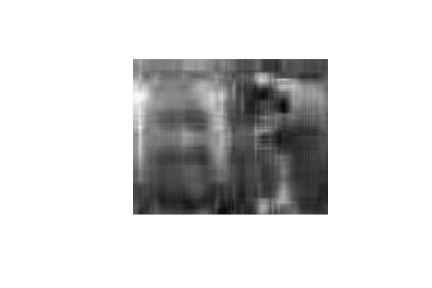
\includegraphics[width=0.45\textwidth]{FIGS/matrix-methods-plot-image-svd-n5-1.png}
\end{center}
\vfill
Uses 1.41\% of the original information
\end{frame}




\begin{frame}\frametitle{Using $n=10$ singular values}
\begin{center}

\includegraphics[width=0.45\textwidth]{FIGS/matrix-methods-plot-image-svd-original-1.png}
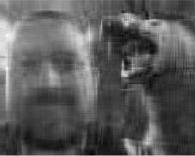
\includegraphics[width=0.45\textwidth]{FIGS/matrix-methods-plot-image-svd-n10-1.png}
\end{center}
\vfill
Uses 2.81\% of the original information
\end{frame}





\begin{frame}\frametitle{Using $n=20$ singular values}
\begin{center}

\includegraphics[width=0.45\textwidth]{FIGS/matrix-methods-plot-image-svd-original-1.png}

\includegraphics[width=0.45\textwidth]{FIGS/matrix-methods-plot-image-svd-n20-1.png}
\end{center}
\vfill
Uses 5.63\% of the original information
\end{frame}





\begin{frame}\frametitle{Using $n=50$ singular values}
\begin{center}

\includegraphics[width=0.45\textwidth]{FIGS/matrix-methods-plot-image-svd-original-1.png}
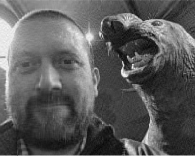
\includegraphics[width=0.45\textwidth]{FIGS/matrix-methods-plot-image-svd-n50-1.png}
\end{center}
\vfill
Uses 14.07\% of the original information
\end{frame}




%%%%%%%%%%%%%%%%%%%%%
%%%%%%%%%%%%%%%%%%%%%
%%%%%%%%%%%%%%%%%%%%%
%%%%%%%%%%%%%%%%%%%%%
\section{Principal component analysis (PCA)}
\newSectionSlide{FIGS/Gemini_Generated_Image_c06eixc06eixc06e.jpeg}


\begin{frame}{Dimensionality reduction}
One of the reasons the SVD is used is for dimensionality reduction. However, SVD has many many other uses
\vfill
Now we look at another dimensionality reduction technique, PCA
\vfill
PCA is often used as a blackbox technique, here we take a look at the math behind it
\end{frame}


\begin{frame}{What is PCA?}
Linear algebraic technique 
\vfill
Helps reduce a complex dataset to a lower dimensional one
\vfill
Non-parametric method: does not assume anything about data distribution (distribution from the statistical point of view)
\end{frame}

%%%%%%%%%%%%%%%%%%%%%
%%%%%%%%%%%%%%%%%%%%%
\subsection{A crash course on probability}
\newSubSectionSlide{FIGS/Gemini_Generated_Image_c06eixc06eixc06e.jpeg}


\begin{frame}{Brief ``review'' of some probability concepts}
Proper definition of \emph{probability} requires to use \emph{measure theory}.. will not get into details here
\vfill
A \textbf{random variable} $X$ is a \emph{measurable} function $X:\Omega\to E$, where $\Omega$ is a set of outcomes (\emph{sample space}) and $E$ is a measurable space
\vfill
$\IP(X\in S\subseteq E) = \IP(\omega\in\Omega|X(\omega)\in S)$
\vfill
\textbf{Distribution function} of a r.v., $F(x)=\IP(X\leq x)$, describes the distribution of a r.v.
\vfill
R.v. can be discrete or continuous or .. other things. 
\end{frame}

\begin{frame}
\begin{definition}[Variance]
Let $X$ be a random variable. The \textbf{variance} of $X$ is given by
\[
\Var X = E\left[\left(X-E(X)\right)^2\right]
\]
where $E$ is the expected value
\end{definition}
\vfill
\begin{definition}[Covariance]
Let $X,Y$ be jointly distributed random variables. The \textbf{covariance} of $X$ and $Y$ is given by
\[
\cov (X,Y) = E\left[\left(X-E(X)\right)\left(Y-E(Y)\right)\right]
\]
\end{definition}
\vfill
Note that $\cov(X,X)=E\left[\left(X-E(X)\right)^2\right] = \Var X$
\end{frame}

\begin{frame}{In practice: ``true law'' versus ``observation''}
In statistics: we reason on the \emph{true law} of distributions, but we usually have only access to a sample
\vfill
We then use \textbf{estimators} to .. estimate the value of a parameter, e.g., the mean, variance and covariance
\vfill
\end{frame}
    
\begin{frame}
\begin{definition}[Unbiased estimators of the mean and variance]
Let $x_1,\ldots,x_n$ be data points (the \emph{sample}) and 
\[
\bar x = \frac 1n \sum_{i=1}^n x_i
\]
be the \textbf{mean} of the data. An unbiased estimator of the variance of the sample is
\[
\sigma^2 = \frac{1}{n-1}\sum_{i=1}^n (x_i-\bar x)^2
\]
\end{definition}
\end{frame}

\begin{frame}
\begin{definition}[Unbiased estimator of the covariance]
Let $(x_1,y_1),\ldots,(x_n,y_n)$ be data points,
\[
\bar x = \frac 1n \sum_{i=1}^n x_i
\textrm{ and }
\bar y = \frac 1n \sum_{i=1}^n y_i
\]
be the means of the data. An estimator of the covariance of the sample is
\[
\cov(x,y) = \frac{1}{n}\sum_{i=1}^n (x_i-\bar x)(y_i-\bar y)
\]
\end{definition}
\end{frame}

\begin{frame}{What does covariance do?}
Variance explains how data disperses around the mean, in a 1-D case
\vfill
Covariance measures the relationship between two dimensions. E.g., height and weight
\vfill
More than the exact value, the sign is important:
\begin{itemize}
    \item $\cov(X,Y)>0$: both dimensions change in the same ``direction''; e.g., larger height usually means higher weight
    \item $\cov(X,Y)<0$: both dimensions change in reverse directions; e.g., time spent on social media and performance in this class
    \item $\cov(X,Y)=0$: the dimensions are independent from one another; e.g., sex/gender and ``intelligence''
\end{itemize}
\end{frame}

\begin{frame}{The covariance matrix}
Typically, we consider more than 2 variables.. 
\begin{definition}
Suppose $p$ random variables $X_1,\ldots,X_p$. Then the covariance matrix is the symmetric matrix
\[
\begin{pmatrix}
\cov(X_1,X_1) & \cov(X_1,X_2) & \cdots & \cov(X_1,X_p) \\
\cov(X_2,X_1) & \cov(X_2,X_2) & \cdots & \cov(X_2,X_p) \\
\vdots & \vdots & & \vdots \\
\cov(X_p,X_1) & \cov(X_p,X_2) & \cdots & \cov(X_p,X_p) 
\end{pmatrix}
\]
i.e., using the properties of covariance,
\[
\begin{pmatrix}
\Var X_1 & \cov(X_1,X_2) & \cdots & \cov(X_1,X_p) \\
\cov(X_1,X_2) & \Var X_2 & \cdots & \cov(X_2,X_p) \\
\vdots & \vdots & & \vdots \\
\cov(X_1,X_p) & \cov(X_2,X_p) & \cdots & \Var X_p 
\end{pmatrix}
\]
\end{definition}
\end{frame}


%%%%%%%%%%%%%%%%%%%%%
%%%%%%%%%%%%%%%%%%%%%
\subsection{A running example: fingerprints}
\newSubSectionSlide{FIGS/Gemini_Generated_Image_7cansa7cansa7can.jpeg}
\begin{frame}{Example of a PCA problem}
We collect a bunch of information about a bunch of people.. for instance this data from Loughborough University
\vfill
\begin{quote}
This dataset contains the height, weight and 4 fingerprint measurements (length, width, area and circumference), collected from 200 participants.
\end{quote}
\vfill
What best describes a participant?
\end{frame}

\begin{frame}{The variables}
Each participant is associated to 11 variables
\vfill
\begin{itemize}
\item "Participant Number"
\item "Gender"
\item "Age"
\item "Dominant Hand"
\item "Height (cm) (average of 3 measurements)"
\item "Weight (kg) (average of 3 measurements)"
\item "Fingertip Temperature (°C)"
\item "Fingerprint Height (mm)"
\item "Fingerprint Width (mm)"
\item "Fingerprint Area (mm2)"
\item "Fingerprint Circumference (mm)"
\end{itemize}
\end{frame}

\begin{frame}{Nature of variables}
Variables have different natures
\vfill
\begin{itemize}
\item "Participant Number": $\in\IN$ (not interesting)
\item "Gender": categorical
\item "Age": $\in\IN$ 
\item "Dominant Hand": categorical
\item "Height (cm) (average of 3 measurements)": $\in\IR$
\item "Weight (kg) (average of 3 measurements)": $\in\IR$
\item "Fingertip Temperature (°C)": $\in\IR$
\item "Fingerprint Height (mm)": $\in\IR$
\item "Fingerprint Width (mm)": $\in\IR$
\item "Fingerprint Area (mm2)": $\in\IR$
\item "Fingerprint Circumference (mm)": $\in\IR$
\end{itemize}
\end{frame}

\begin{frame}{Setting things up}
Each participant is a row in the matrix (an \emph{observation})
\vfill
Each variable is a column
\vfill
So we have an $200\times 10$ matrix (we discard the ``Participant number'' column)
\vfill
We want to find what carries the most information
\vfill
For this, we are going to project the information in a new basis in which the first ``dimension'' will carry most variance, the second dimension will carry a little less, etc.
\vfill
In order to do so, we need to learn how to change bases
\end{frame}

%%%%%%%%%%%%%%%%%%%%%
%%%%%%%%%%%%%%%%%%%%%
\subsection{Change of basis}
\newSubSectionSlide{FIGS/Gemini_Generated_Image_c06eixc06eixc06e.jpeg}
\begin{frame}
	In the following slide, 
	\[
	[\bx]_\B
	\]
	denotes the coordinates of $\bx$ in the basis $\B$
	\vfill
	The aim of a change of basis is to express vectors in another coordinate system (another basis)
	\vfill
	We do so by finding a matrix allowing to move from one basis to another
\end{frame}

\begin{frame}{Change of basis}
\begin{definition}[Change of basis matrix]
$\B=\{\bu_1,\ldots,\bu_n\}$ and $\C=\{\bv_1,\ldots,\bv_n\}$ bases of vector space $V$
\vfill
The \textbf{change of basis matrix} $P_{\C\leftarrow\B}\in\M_n$,
\[
P_{\C\leftarrow\B}
=\left[
[\bu_1]_\C \cdots [\bu_n]_\C
\right]
\]
has columns the coordinate vectors $[\bu_1]_\C,\ldots,[\bu_n]_\C$ of vectors in $\B$ with respect to $\C$
\end{definition}
\vfill
\begin{theorem}
$\B=\{\bu_1,\ldots,\bu_n\}$ and $\C=\{\bv_1,\ldots,\bv_n\}$ bases of vector space $V$ and $P_{\C\leftarrow\B}$ a change of basis matrix from $\B$ to $\C$
\begin{enumerate}
\item $\forall\bx\in V$, $P_{\C\leftarrow\B}[\bx]_\B = [\bx]_\C$
\item $P_{\C\leftarrow\B}$ s.t. $\forall\bx\in V$, $P_{\C\leftarrow\B}[\bx]_\B = [\bx]_\C$ is \textbf{unique}
\item $P_{\C\leftarrow\B}$ invertible and $P_{\C\leftarrow\B}^{-1}=P_{\B\leftarrow\C}$
\end{enumerate}
\end{theorem}
\end{frame}


\begin{frame}{Row-reduction method for changing bases}
\begin{theorem}
\label{th:change-basis-construction}
$\B=\{\bu_1,\ldots,\bu_n\}$ and $\C=\{\bv_1,\ldots,\bv_n\}$ bases of vector space $V$. Let $\E$ be any basis for $V$,
\[
B = [[\bu_1]_\E,\ldots,[\bu_n]_\E] 
\textrm{ and }
C = [[\bv_1]_\E,\ldots,[\bv_n]_\E] 
\]
and let $[C|B]$ be the augmented matrix constructed using $C$ and $B$. Then
\[
RREF\left([C|B]\right)
=[\II|P_{\C\leftarrow\B}]
\]
\end{theorem}
\vfill
If working in $\IR^n$, this is quite useful with $\E$ the standard basis of $\IR^n$ (it does not matter if $\B=\E$)
\end{frame}

\begin{frame}
So the question now becomes
\begin{quote}
How do we find what new basis to look at our data in?
\end{quote}
\vfill
(Changing the basis does not change the data, just the view you have of it)
\vfill
(Think of what happens when you do a headstand.. your up becomes down, your right and left switch, but the world does not change, just your view of it)
\vfill
(Changes of bases are \emph{fundamental} operations in Science)
\end{frame}



%%%%%%%%%%%%%%%%%%%%%
%%%%%%%%%%%%%%%%%%%%%
\subsection{Back to PCA}
\newSubSectionSlide{FIGS/Gemini_Generated_Image_c06eixc06eixc06e.jpeg}
\begin{frame}{Setting things up}
I will use notation (mostly) as in Joliffe's \emph{Principal Component Analysis} (PDF of older version available for free from UofM Libraries)
\vfill
$\bx=(x_1,\ldots,x_p)$ vector of $p$ random variables
\end{frame}


\begin{frame} 
We seek a linear function $\bm{\alpha}_1^T\bx$ with maximum variance, where $\bm{\alpha}_1=(\alpha_{11},\ldots,\alpha_{1p})$, i.e.,
\[
\bm{\alpha}_1^T\bx = \sum_{j=1}^p\alpha_{1j}x_j
\]
\vfill
Then we seek a linear function $\bm{\alpha}_2^T\bx$ with maximum variance, uncorrelated to $\bm{\alpha}_1^T\bx$
\vfill
And we continue...
\vfill
At $k$th stage, we find a linear function $\bm{\alpha}_k^T\bx$ with maximum variance, uncorrelated to $\bm{\alpha}_1^T\bx,\ldots,\bm{\alpha}_{k-1}^T\bx$
\vfill
$\bm{\alpha}_i^T\bx$ is the $i$th \textbf{principal component} (PC)
\end{frame}

\begin{frame}{Case of known covariance matrix}
Suppose we know $\Sigma$, covariance matrix of $\bx$ (i.e., typically: we know $\bx$)
\vfill
Then the $k$th PC is 
\[
z_k=\bm{\alpha}_k^T\bx
\]
where $\bm{\alpha}_k$ is an eigenvector of $\Sigma$ corresponding to the $k$th largest eigenvalue $\lambda_k$
\vfill
If, additionally, $\|\bm{\alpha}_k\|=\bm{\alpha}_k^T\bm{\alpha}=1$, then $\lambda_k=\Var z_k$
\end{frame}


\begin{frame}{Why is that?}
Let us start with
\[
\bm{\alpha}_1^T\bx
\]
\vfill
We want maximum variance, where $\bm{\alpha}_1=(\alpha_{11},\ldots,\alpha_{1p})$, i.e.,
\[
\bm{\alpha}_1^T\bx = \sum_{j=1}^p\alpha_{1j}x_j
\]
with the constraint that $\|\bm{\alpha}_1\|=1$
\vfill
We have
\[
\Var \bm{\alpha}_1^T\bx
=\bm{\alpha}_1^T\Sigma\bm{\alpha}_1
\]
\end{frame}

\begin{frame}{Objective}
We want to maximise $\Var \bm{\alpha}_1^T\bx$, i.e.,
\[
\bm{\alpha}_1^T\Sigma\bm{\alpha}_1
\]
under the constraint that $\|\bm{\alpha}_1\|=1$
\vfill
$\implies$ use \textbf{Lagrange multipliers}
\end{frame}


\begin{frame}{Maximisation using Lagrange multipliers}
\framesubtitle{(A.k.a. super-brief intro to multivariable calculus)}
We want the max of $f(x_1,\ldots,x_n)$ under the constraint $g(x_1,\ldots,x_n)=k$
\begin{enumerate}
\item Solve
\begin{align*}
\nabla f(x_1,\ldots,x_n) &= \lambda\nabla g(x_1,\ldots,x_n) \\
g(x_1,\ldots,x_n) &= k
\end{align*}
where $\nabla=(\frac{\partial}{\partial x_1},\ldots,\frac{\partial}{\partial x_n})$ is the \textbf{gradient operator}
\item Plug all solutions into $f(x_1,\ldots,x_n)$ and find maximum values (provided values exist and $\nabla g\neq \b0$ there)
\end{enumerate}
\vfill
$\lambda$ is the \textbf{Lagrange multiplier}
\end{frame}


\begin{frame}{The gradient}
\framesubtitle{(Continuing our super-brief intro to multivariable calculus)}
$f:\IR^n\to\IR$ function of several variables, $\nabla=\left(\frac{\partial}{\partial x_1},\ldots,\frac{\partial}{\partial x_n}\right)$ the gradient operator
\vfill
Then
\[
\nabla f = \left(
\frac{\partial}{\partial x_1}f,\ldots,
\frac{\partial}{\partial x_n}f
\right)
\]
\vfill
So $\nabla f$ is a \emph{vector-valued} function, $\nabla f:\IR^n\to\IR^n$; also written as
\[
\nabla f = f_{x_1}(x_1,\ldots,x_n)\be_1+\cdots f_{x_n}(x_1,\ldots,x_n)\be_n
\]
where $f_{x_i}$ is the partial derivative of $f$ with respect to $x_i$ and $\{\be_1,\ldots,\be_n\}$ is the standard basis of $\IR^n$
\end{frame}


\begin{frame}{Bear with me..}
\framesubtitle{(You may experience a brief period of discomfort)}
$\bm{\alpha}_1^T\Sigma\bm{\alpha}_1$ and $\|\bm{\alpha}_1\|^2=\bm{\alpha}_1^T\bm{\alpha_1}$ are functions of $\bm{\alpha}_1=(\alpha_{11},\ldots,\alpha_{1p})$
\vfill
In the notation of the previous slide, we want the max of 
\[
f(\alpha_{11},\ldots,\alpha_{1p}) := \bm{\alpha}_1^T\Sigma\bm{\alpha}_1
\]
under the constraint that
\[
g(\alpha_{11},\ldots,\alpha_{1p}) := \bm{\alpha}_1^T\bm{\alpha_1} = 1
\]
and with gradient operator
\[
\nabla = \left(
\frac{\partial}{\partial \alpha_{11}},
\ldots,
\frac{\partial}{\partial \alpha_{1p}}
\right)
\]
\end{frame}


\begin{frame}{Effect of $\nabla$ on $g$}
$g$ is easiest to see:
\begin{align*}
\nabla g(\alpha_{11},\ldots,\alpha_{1p}) &=
\left(
\frac{\partial}{\partial \alpha_{11}},
\ldots,
\frac{\partial}{\partial \alpha_{1p}}
\right) (\alpha_{11},\ldots,\alpha_{1p}) 
\begin{pmatrix}
\alpha_{11}\\ \vdots\\ \alpha_{1p}
\end{pmatrix} \\
&= \left(
\frac{\partial}{\partial \alpha_{11}},
\ldots,
\frac{\partial}{\partial \alpha_{1p}}
\right) 
\left(
\alpha_{11}^2+\cdots+\alpha_{1p}^2
\right) \\
&= \left(2\alpha_{11},\ldots,2\alpha_{1p}\right)\\
&= 2\bm{\alpha}_1
\end{align*}
\vfill
(And that's a general result: $\nabla\|\bx\|_2^2=2\bx$ with $\|\cdot\|_2$ the Euclidean norm)
\end{frame}

\begin{frame}{Effect of $\nabla$ on $f$}
Expand (write $\Sigma=[s_{ij}]$ and do not exploit symmetry)
\begin{align*}
\bm{\alpha}_1^T\Sigma\bm{\alpha}_1 &=
\left(\alpha_{11},\ldots,\alpha_{1p}\right)
\begin{pmatrix}
s_{11} & s_{12} & \cdots & s_{1p} \\
s_{21} & s_{22} & \cdots & s_{2p} \\
\vdots & \vdots & & \vdots \\
s_{p1} & s_{p2} & & s_{pp}
\end{pmatrix}
\begin{pmatrix}
\alpha_{11} \\ \alpha_{12} \\ \vdots \\ \alpha_{1p}
\end{pmatrix} \\
&=
\left(\alpha_{11},\ldots,\alpha_{1p}\right)
\begin{pmatrix}
s_{11}\alpha_{11}+s_{12}\alpha_{12}+\cdots+s_{1p}\alpha_{1p} \\
s_{21}\alpha_{11}+s_{22}\alpha_{12}+\cdots+s_{2p}\alpha_{1p} \\
\vdots \\
s_{p1}\alpha_{11}+s_{p2}\alpha_{12}+\cdots+s_{pp}\alpha_{1p}
\end{pmatrix} \\
&=
(s_{11}\alpha_{11}+s_{12}\alpha_{12}+\cdots+s_{1p}\alpha_{1p})\alpha_{11} \\
&\quad +
(s_{21}\alpha_{11}+s_{22}\alpha_{12}+\cdots+s_{2p}\alpha_{1p})\alpha_{12} \\
&\quad\;\;\vdots \\
&\quad +
(s_{p1}\alpha_{11}+s_{p2}\alpha_{12}+\cdots+s_{pp}\alpha_{1p})\alpha_{1p}
\end{align*}
\end{frame}

\begin{frame}
We have
\begin{align*}
\bm{\alpha}_1^T\Sigma\bm{\alpha}_1 &=
(s_{11}\alpha_{11}+s_{12}\alpha_{12}+\cdots+s_{1p}\alpha_{1p})\alpha_{11} \\
&\quad +
(s_{21}\alpha_{11}+s_{22}\alpha_{12}+\cdots+s_{2p}\alpha_{1p})\alpha_{12} \\
&\quad\;\;\vdots \\
&\quad +
(s_{p1}\alpha_{11}+s_{p2}\alpha_{12}+\cdots+s_{pp}\alpha_{1p})\alpha_{1p} 
\end{align*}
\begin{align*}
\implies\frac{\partial}{\partial \alpha_{11}}
\bm{\alpha}_1^T\Sigma\bm{\alpha}_1  
&= 
(s_{11}\alpha_{11}+s_{12}\alpha_{12}+\cdots+s_{1p}\alpha_{1p})+s_{11}\alpha_{11} \\
&\quad + s_{21}\alpha_{12} +\cdots + s_{p1}\alpha_{1p} \\
&= s_{11}\alpha_{11}+s_{12}\alpha_{12}+\cdots+s_{1p}\alpha_{1p} \\
&\quad+
s_{11}\alpha_{11}+s_{21}\alpha_{12}+\cdots+s_{p1}\alpha_{1p} \\
&= 2(s_{11}\alpha_{11}+s_{12}\alpha_{12}+\cdots+s_{1p}\alpha_{1p})
\end{align*}
(last equality stems from symmetry of $\Sigma$)
\end{frame}

\begin{frame}
In general, for $i=1,\ldots,p$,
\begin{align*}
\frac{\partial}{\partial \alpha_{1i}}
\bm{\alpha}_1^T\Sigma\bm{\alpha}_1  
&= s_{i1}\alpha_{11}+s_{i2}\alpha_{12}+\cdots+s_{ip}\alpha_{1p}\\
&\quad+s_{i1}\alpha_{11}+s_{2i}\alpha_{12}+\cdots+s_{pi}\alpha_{1p} \\
&= 2(s_{i1}\alpha_{11}+s_{i2}\alpha_{12}+\cdots+s_{ip}\alpha_{1p})
\end{align*}
(because of symmetry of $\Sigma$)
\vfill
As a consequence,
\[
\nabla \bm{\alpha}_1^T\Sigma\bm{\alpha}_1
=2\Sigma\bm{\alpha}_1
\]
\end{frame}

\begin{frame}
So solving
\[
\nabla f(x_1,\ldots,x_n) = \lambda\nabla g(x_1,\ldots,x_n) 
\]
means solving
\[
2\Sigma\bm{\alpha}_1 = \lambda 2\bm{\alpha}_1 
\]
i.e.,
\[
\Sigma\bm{\alpha}_1 = \lambda\bm{\alpha}_1 
\]
\vfill
$\implies$
$(\lambda,\bm{\alpha}_1)$ eigenpair of $\Sigma$, with $\bm{\alpha}_1$ having unit length
\end{frame}


\begin{frame}{Picking the right eigenvalue}
$(\lambda,\bm{\alpha}_1)$ eigenpair of $\Sigma$, with $\bm{\alpha}_1$ having unit length
\vfill
But which $\lambda$ to choose?
\vfill
Recall that we want $\Var \bm{\alpha}_1^T\bx=\bm{\alpha}_1^T\Sigma\bm{\alpha}_1$ maximal
\vfill
We have
\[
\Var \bm{\alpha}_1^T\bx 
= \bm{\alpha}_1^T\Sigma\bm{\alpha}_1 
= \bm{\alpha}_1^T(\Sigma\bm{\alpha}_1) 
= \bm{\alpha}_1^T(\lambda\bm{\alpha}_1) 
= \lambda(\bm{\alpha}_1^T\bm{\alpha}_1) = \lambda
\]
\vfill
$\implies$ we pick $\lambda=\lambda_1$, the largest eigenvalue (covariance matrix symmetric so eigenvalues real)
\end{frame}


\begin{frame}{What we have this far..}
The first principal component is $\bm{\alpha}_1^T\bx$ and has variance $\lambda_1$, where $\lambda_1$ the largest eigenvalue of $\Sigma$ and $\bm{\alpha}_1$ an associated eigenvector with $\|\bm{\alpha}_1\|=1$
\vfill
We want the second principal component to be \emph{uncorrelated} with $\bm{\alpha}_1^T\bx$ and to have maximum variance $\Var \bm{\alpha}_2^T\bx=\bm{\alpha}_2^T\Sigma\bm{\alpha}_2$, under the constraint that $\|\bm{\alpha}_2\|=1$
\vfill
$\bm{\alpha}_2^T\bx$ uncorrelated to $\bm{\alpha}_1^T\bx$ if $\cov(\bm{\alpha}_1^T\bx,\bm{\alpha}_2^T\bx)=0$
\end{frame}

\begin{frame}
We have
\begin{align*}
\cov(\bm{\alpha}_1^T\bx,\bm{\alpha}_2^T\bx) &= 
\bm{\alpha}_1^T\Sigma\bm{\alpha}_2 \\
&= \bm{\alpha}_2^T\Sigma^T\bm{\alpha}_1 \\
&= \bm{\alpha}_2^T\Sigma\bm{\alpha}_1 \quad\textrm{[$\Sigma$ symmetric]} \\
&= \bm{\alpha}_2^T(\lambda_1\bm{\alpha}_1) \\
&= \lambda \bm{\alpha}_2^T\bm{\alpha}_1
\end{align*}
\vfill
So $\bm{\alpha}_2^T\bx$ uncorrelated to $\bm{\alpha}_1^T\bx$ if $\bm{\alpha}_1\perp\bm{\alpha}_2$
\vfill
This is beginning to sound a lot like Gram-Schmidt, no?
\end{frame}

\begin{frame}{In short}
Take whatever covariance matrix is available to you (known $\Sigma$ or sample $S_X$) -- assume sample from now on for simplicity
\vfill
For $i=1,\ldots,p$, the $i$th principal component is
\[
z_i = \bv_i^T\bx
\]
where $\bv_i$ eigenvector of $S_X$ associated to the $i$th largest eigenvalue $\lambda_i$
\vfill
If $\bv_i$ is normalised, then $\lambda_i=\Var z_k$
\end{frame}


\begin{frame}{Covariance matrix}
$\Sigma$ the covariance matrix of the random variable, $S_X$ the sample covariance matrix
\vfill
$X\in\M_{mp}$ the data, then the (sample) covariance matrix $S_X$ takes the form
\[
S_X = \frac{1}{n-1}X^TX
\]
where the data is centred!
\vfill
Sometimes you will see $S_X=1/(n-1)XX^T$. This is for matrices with observations in columns and variables in rows. Just remember that you want the covariance matrix to have size the number of variables, not observations, this will give you the order in which to take the product
\end{frame}

%%%%%%%%%%%%%%%%%%%%%
%%%%%%%%%%%%%%%%%%%%%
\subsection{A 2D example to begin: hockey players}
\newSubSectionSlide{FIGS/Gemini_Generated_Image_ee8lhqee8lhqee8l.jpeg}

\begin{frame}[fragile]{A 2D example}
See a dataset \href{https://opendata.stackexchange.com/questions/7793/age-weight-and-height-dataset}{on this page} for a dataset of height and weight of some hockey players
\vfill
\begin{knitrout}
\definecolor{shadecolor}{rgb}{0.969, 0.969, 0.969}\color{fgcolor}\begin{kframe}
\begin{alltt}
\hldef{data} \hlkwb{=} \hlkwd{read.csv}\hldef{(}\hlsng{"https://figshare.com/ndownloader/files/5303173"}\hldef{)}
\hlkwd{head}\hldef{(data,} \hlkwc{n}\hldef{=}\hlnum{3}\hldef{)}
\end{alltt}
\begin{verbatim}
##   year country no                name position side height weight      birth
## 1 2001     RUS 10    tverdovsky oleg         D    L    185     84 1976-05-18
## 2 2001     RUS  2  vichnevsky vitali         D    L    188     86 1980-03-18
## 3 2001     RUS 26 petrochinin evgeni         D    L    182     95 1976-02-07
##                      club      age cohort      bmi
## 1   anaheim mighty ducks  24.95277   1976 24.54346
## 2   anaheim mighty ducks  21.11978   1980 24.33228
## 3 severstal cherepovetal  25.22930   1976 28.68011
\end{verbatim}
\begin{alltt}
\hlkwd{dim}\hldef{(data)}
\end{alltt}
\begin{verbatim}
## [1] 6292   13
\end{verbatim}
\end{kframe}
\end{knitrout}
\end{frame}

\begin{frame}
In case you are wondering, this is a database of ice hockey players at IIHF world championships, 2001-2016, assembled by the dataset's author
\vfill
See some comments \href{https://ikashnitsky.github.io/2017/ice-hockey-players-height/}{here}
\vfill
As usual, it is a good idea to plot this to get a sense of the lay of the land
\end{frame}




\maxFrameImage{FIGS/matrix-methods-plot-hockey-1-1.pdf}

\begin{frame}[fragile]
The author of the study is interested in the evolution of weights, so it is likely that the same person will be in the dataset several times
\vfill
Let us check this: first check will be \code{FALSE} if the number of unique names does not match the number of rows in the dataset

\begin{knitrout}
\definecolor{shadecolor}{rgb}{0.969, 0.969, 0.969}\color{fgcolor}\begin{kframe}
\begin{alltt}
\hlkwd{length}\hldef{(}\hlkwd{unique}\hldef{(data}\hlopt{$}\hldef{name))} \hlopt{==} \hlkwd{dim}\hldef{(data)[}\hlnum{1}\hldef{]}
\end{alltt}
\begin{verbatim}
## [1] FALSE
\end{verbatim}
\begin{alltt}
\hlkwd{length}\hldef{(}\hlkwd{unique}\hldef{(data}\hlopt{$}\hldef{name))}
\end{alltt}
\begin{verbatim}
## [1] 3278
\end{verbatim}
\end{kframe}
\end{knitrout}
\end{frame}

\begin{frame}[fragile]
Not interested in the evolution of weights, so simplify: if more than one record for someone, take average of recorded weights and heights
\vfill
To be extra careful, could check as well that there are no major variations on player height (homonymies?)
\vfill
\begin{knitrout}
\definecolor{shadecolor}{rgb}{0.969, 0.969, 0.969}\color{fgcolor}\begin{kframe}
\begin{alltt}
\hldef{data_simplified} \hlkwb{=} \hlkwd{data.frame}\hldef{(}\hlkwc{name} \hldef{=} \hlkwd{unique}\hldef{(data}\hlopt{$}\hldef{name))}
\hldef{w} \hlkwb{=} \hlkwd{c}\hldef{()}
\hldef{h} \hlkwb{=} \hlkwd{c}\hldef{()}
\hlkwa{for} \hldef{(n} \hlkwa{in} \hldef{data_simplified}\hlopt{$}\hldef{name) \{}
    \hldef{tmp} \hlkwb{=} \hldef{data[}\hlkwd{which}\hldef{(data}\hlopt{$}\hldef{name} \hlopt{==} \hldef{n),]}
    \hldef{h} \hlkwb{=} \hlkwd{c}\hldef{(h,} \hlkwd{mean}\hldef{(tmp}\hlopt{$}\hldef{height))}
    \hldef{w} \hlkwb{=} \hlkwd{c}\hldef{(w,} \hlkwd{mean}\hldef{(tmp}\hlopt{$}\hldef{weight))}
\hldef{\}}
\hldef{data_simplified}\hlopt{$}\hldef{weight} \hlkwb{=} \hldef{w}
\hldef{data_simplified}\hlopt{$}\hldef{height} \hlkwb{=} \hldef{h}
\end{alltt}
\end{kframe}
\end{knitrout}
\end{frame}

\begin{frame}[fragile]
\begin{knitrout}
\definecolor{shadecolor}{rgb}{0.969, 0.969, 0.969}\color{fgcolor}\begin{kframe}
\begin{alltt}
\hldef{data} \hlkwb{=} \hldef{data_simplified}
\hlkwd{head}\hldef{(data_simplified,} \hlkwc{n} \hldef{=} \hlnum{6}\hldef{)}
\end{alltt}
\begin{verbatim}
##                  name weight height
## 1    tverdovsky oleg    84.0  185.0
## 2  vichnevsky vitali    86.0  188.0
## 3 petrochinin evgeni    95.0  182.0
## 4    zhdan alexander    85.5  178.5
## 5    orekhovsky oleg    88.0  175.0
## 6      zhukov sergei    92.5  193.0
\end{verbatim}
\end{kframe}
\end{knitrout}
\end{frame}



\maxFrameImage{FIGS/matrix-methods-plot-hockey-2-1.pdf}

\begin{frame}[fragile]\frametitle{Centre the data}
\begin{knitrout}
\definecolor{shadecolor}{rgb}{0.969, 0.969, 0.969}\color{fgcolor}\begin{kframe}
\begin{alltt}
\hlkwd{mean}\hldef{(data}\hlopt{$}\hldef{weight)}
\end{alltt}
\begin{verbatim}
## [1] 87.71555
\end{verbatim}
\begin{alltt}
\hlkwd{mean}\hldef{(data}\hlopt{$}\hldef{height)}
\end{alltt}
\begin{verbatim}
## [1] 183.8596
\end{verbatim}
\begin{alltt}
\hldef{data}\hlopt{$}\hldef{weight.c} \hlkwb{=} \hldef{data}\hlopt{$}\hldef{weight}\hlopt{-}\hlkwd{mean}\hldef{(data}\hlopt{$}\hldef{weight)}
\hldef{data}\hlopt{$}\hldef{height.c} \hlkwb{=} \hldef{data}\hlopt{$}\hldef{height}\hlopt{-}\hlkwd{mean}\hldef{(data}\hlopt{$}\hldef{height)}
\end{alltt}
\end{kframe}
\end{knitrout}
\end{frame}

\maxFrameImage{FIGS/matrix-methods-plot-hockey-centred-1.pdf}



\begin{frame}[fragile]\frametitle{Covariance}
The function \code{cov} returns the covariance of two samples
\vfill
Note that the functions deals equally well with data that is not centred as with data that is centred
\vfill
\begin{knitrout}
\definecolor{shadecolor}{rgb}{0.969, 0.969, 0.969}\color{fgcolor}\begin{kframe}
\begin{alltt}
\hlkwd{cov}\hldef{(data}\hlopt{$}\hldef{height, data}\hlopt{$}\hldef{weight)}
\end{alltt}
\begin{verbatim}
## [1] 26.63506
\end{verbatim}
\begin{alltt}
\hlkwd{cov}\hldef{(data}\hlopt{$}\hldef{height.c, data}\hlopt{$}\hldef{weight.c)}
\end{alltt}
\begin{verbatim}
## [1] 26.63506
\end{verbatim}
\end{kframe}
\end{knitrout}
\end{frame}


\begin{frame}[fragile]\frametitle{Covariance matrix}
As we could see from plotting the data, there is a positive linear relationship between the two variables
\vfill
Let us compute the sample covariance matrix
\vfill
\begin{knitrout}
\definecolor{shadecolor}{rgb}{0.969, 0.969, 0.969}\color{fgcolor}\begin{kframe}
\begin{alltt}
\hldef{X} \hlkwb{=} \hlkwd{as.matrix}\hldef{(data[,}\hlkwd{c}\hldef{(}\hlsng{"height.c"}\hldef{,} \hlsng{"weight.c"}\hldef{)])}
\hldef{S} \hlkwb{=} \hlnum{1}\hlopt{/}\hldef{(}\hlkwd{dim}\hldef{(X)[}\hlnum{1}\hldef{]}\hlopt{-}\hlnum{1}\hldef{)}\hlopt{*}\hlkwd{t}\hldef{(X)} \hlopt \hldef{X}
\hldef{S}
\end{alltt}
\begin{verbatim}
##          height.c weight.c
## height.c 29.66176 26.63506
## weight.c 26.63506 47.81112
\end{verbatim}
\end{kframe}
\end{knitrout}
\end{frame}

\begin{frame}[fragile]\frametitle{Covariance matrix}
The off-diagonal entries do match the computed covariance. Let us check that the variances are indeed a match too.


\begin{knitrout}
\definecolor{shadecolor}{rgb}{0.969, 0.969, 0.969}\color{fgcolor}\begin{kframe}
\begin{alltt}
\hlkwd{var}\hldef{(X[,}\hlnum{1}\hldef{])}
\end{alltt}
\begin{verbatim}
## [1] 29.66176
\end{verbatim}
\begin{alltt}
\hlkwd{var}\hldef{(X[,}\hlnum{2}\hldef{])}
\end{alltt}
\begin{verbatim}
## [1] 47.81112
\end{verbatim}
\end{kframe}
\end{knitrout}


Hey, that works. Is math not cool? ;)
\end{frame}


\begin{frame}[fragile]\frametitle{Principal components}
Now compute the principal components. We need eigenvalues and eigenvectors
\vfill
\begin{knitrout}
\definecolor{shadecolor}{rgb}{0.969, 0.969, 0.969}\color{fgcolor}\begin{kframe}
\begin{alltt}
\hldef{ev} \hlkwb{=} \hlkwd{eigen}\hldef{(S)}
\hldef{ev}
\end{alltt}
\begin{verbatim}
## eigen() decomposition
## $values
## [1] 66.87496 10.59793
## 
## $vectors
##           [,1]       [,2]
## [1,] 0.5820222 -0.8131729
## [2,] 0.8131729  0.5820222
\end{verbatim}
\end{kframe}
\end{knitrout}
\vfill
(\code{eigen} returns eigenvalues sorted in decreasing order and normalised eigenvectors)
\end{frame}



\begin{frame}[fragile]\frametitle{First principal component}
Let us plot this first eigenvector (well, the line carrying this first eigenvector) 
\vfill
To use the function \code{abline}, we need to give the coefficients of the line in the form of (intercept,slope). Intercept is easy, as the line goes through the origin (by construction and because we have centred the data). The slope is also quite simple..
\vfill
\begin{knitrout}
\definecolor{shadecolor}{rgb}{0.969, 0.969, 0.969}\color{fgcolor}\begin{kframe}
\begin{alltt}
\hlkwd{plot}\hldef{(data}\hlopt{$}\hldef{height.c, data}\hlopt{$}\hldef{weight.c,}
    \hlkwc{pch} \hldef{=} \hlnum{19}\hldef{,} \hlkwc{col} \hldef{=} \hlsng{"dodgerblue4"}\hldef{,}
    \hlkwc{main} \hldef{=} \hlsng{"IIHF players 2001-2016 (with first component)"}\hldef{,}
    \hlkwc{xlab} \hldef{=} \hlsng{"Height (cm)"}\hldef{,} \hlkwc{ylab} \hldef{=} \hlsng{"Weight (kg)"}\hldef{)}
\hlkwd{abline}\hldef{(}\hlkwc{a} \hldef{=} \hlnum{0}\hldef{,} \hlkwc{b} \hldef{= ev}\hlopt{$}\hldef{vectors[}\hlnum{2}\hldef{,}\hlnum{1}\hldef{]}\hlopt{/}\hldef{ev}\hlopt{$}\hldef{vectors[}\hlnum{1}\hldef{,}\hlnum{1}\hldef{],}
       \hlkwc{col} \hldef{=} \hlsng{"red"}\hldef{,} \hlkwc{lwd} \hldef{=} \hlnum{3}\hldef{)}
\end{alltt}
\end{kframe}
\end{knitrout}
\end{frame}

\maxFrameImage{FIGS/matrix-methods-plot-hockey-centred-evector-1.pdf}

\begin{frame}[fragile]\frametitle{Rotating the data}
Let us rotate the data so that the red line becomes the $x$-axis
\vfill
To do that, we use a rotation matrix
$$
R_\theta = \begin{pmatrix}
\cos\theta & -\sin\theta \\
\sin\theta & \cos\theta
\end{pmatrix}
$$
\vfill
To find the angle $\theta$, recall that $\tan\theta$ is equal to opposite length over adjacent length, i.e.,
$$
\tan\theta = \frac{\tt ev\$vectors[2,1]}{\tt ev\$vectors[1,1]}
$$
So we just use the $\arctan$ of this 
\vfill 
Note that angles are in radians
\end{frame}


\begin{frame}[fragile]\frametitle{Rotating the data}
\begin{knitrout}
\definecolor{shadecolor}{rgb}{0.969, 0.969, 0.969}\color{fgcolor}\begin{kframe}
\begin{alltt}
\hldef{theta} \hlkwb{=} \hlkwd{atan}\hldef{(ev}\hlopt{$}\hldef{vectors[}\hlnum{2}\hldef{,}\hlnum{1}\hldef{]}\hlopt{/}\hldef{ev}\hlopt{$}\hldef{vectors[}\hlnum{1}\hldef{,}\hlnum{1}\hldef{])}
\hldef{theta}
\end{alltt}
\begin{verbatim}
## [1] 0.949583
\end{verbatim}
\begin{alltt}
\hldef{R_theta} \hlkwb{=} \hlkwd{matrix}\hldef{(}\hlkwd{c}\hldef{(}\hlkwd{cos}\hldef{(theta),} \hlopt{-}\hlkwd{sin}\hldef{(theta),}
                  \hlkwd{sin}\hldef{(theta),} \hlkwd{cos}\hldef{(theta)),}
                \hlkwc{nr} \hldef{=} \hlnum{2}\hldef{,} \hlkwc{byrow} \hldef{=} \hlnum{TRUE}\hldef{)}
\hldef{R_theta}
\end{alltt}
\begin{verbatim}
##           [,1]       [,2]
## [1,] 0.5820222 -0.8131729
## [2,] 0.8131729  0.5820222
\end{verbatim}
\end{kframe}
\end{knitrout}
\end{frame}


\begin{frame}[fragile]\frametitle{Rotating the data}
And now we rotate the points
\vfill
(In this case, we think of the points as vectors, of course)
\vfill
\begin{knitrout}
\definecolor{shadecolor}{rgb}{0.969, 0.969, 0.969}\color{fgcolor}\begin{kframe}
\begin{alltt}
\hldef{tmp_in} \hlkwb{=} \hlkwd{matrix}\hldef{(}\hlkwd{c}\hldef{(data}\hlopt{$}\hldef{weight.c, data}\hlopt{$}\hldef{height.c),}
                \hlkwc{nc} \hldef{=} \hlnum{2}\hldef{)}
\hldef{tmp_out} \hlkwb{=} \hlkwd{c}\hldef{()}
\hlkwa{for} \hldef{(i} \hlkwa{in} \hlnum{1}\hlopt{:}\hlkwd{dim}\hldef{(tmp_in)[}\hlnum{1}\hldef{]) \{}
    \hldef{tmp_out} \hlkwb{=} \hlkwd{rbind}\hldef{(tmp_out,}
                    \hlkwd{t}\hldef{(R_theta} \hlopt \hldef{tmp_in[i,]))}
\hldef{\}}
\hldef{data}\hlopt{$}\hldef{weight.c_r} \hlkwb{=} \hldef{tmp_out[,}\hlnum{1}\hldef{]}
\hldef{data}\hlopt{$}\hldef{height.c_r} \hlkwb{=} \hldef{tmp_out[,}\hlnum{2}\hldef{]}
\end{alltt}
\end{kframe}
\end{knitrout}
\end{frame}




\maxFrameImage{FIGS/matrix-methods-plot-hockey-centred-evector-2-1.pdf}


\begin{frame}[fragile]\frametitle{Principal components}
Note that the axes have changed quite a lot, hence the very different aspect
\vfill
Let us plot with the same range as for the non-rotated data for the y-axis
\vfill

\begin{knitrout}
\definecolor{shadecolor}{rgb}{0.969, 0.969, 0.969}\color{fgcolor}\begin{kframe}
\begin{alltt}
\hlkwd{plot}\hldef{(data}\hlopt{$}\hldef{height.c_r, data}\hlopt{$}\hldef{weight.c_r,}
    \hlkwc{pch} \hldef{=} \hlnum{19}\hldef{,} \hlkwc{col} \hldef{=} \hlsng{"dodgerblue4"}\hldef{,}
    \hlkwc{xlab} \hldef{=} \hlsng{"x-axis"}\hldef{,} \hlkwc{ylab} \hldef{=} \hlsng{"y-axis"}\hldef{,}
    \hlkwc{main} \hldef{=} \hlsng{"IIHF players 2001-2016 (rotated to first component)"}\hldef{,}
    \hlkwc{ylim} \hldef{=} \hlkwd{range}\hldef{(data}\hlopt{$}\hldef{weight.c))}
\hlkwd{abline}\hldef{(}\hlkwc{h} \hldef{=} \hlnum{0}\hldef{,} \hlkwc{col} \hldef{=} \hlsng{"red"}\hldef{,} \hlkwc{lwd} \hldef{=} \hlnum{2}\hldef{)}
\end{alltt}
\end{kframe}
\end{knitrout}
\end{frame}


\maxFrameImage{FIGS/matrix-methods-plot-hockey-centred-rotated-1.pdf}


\begin{frame}[fragile]\frametitle{First and second principal components}
Plot the first and second eigenvectors
\vfill
\begin{knitrout}
\definecolor{shadecolor}{rgb}{0.969, 0.969, 0.969}\color{fgcolor}\begin{kframe}
\begin{alltt}
\hlkwd{plot}\hldef{(data}\hlopt{$}\hldef{height.c, data}\hlopt{$}\hldef{weight.c,}
    \hlkwc{pch} \hldef{=} \hlnum{19}\hldef{,} \hlkwc{col} \hldef{=} \hlsng{"dodgerblue4"}\hldef{,}
    \hlkwc{main} \hldef{=} \hlsng{"IIHF players 2001-2016 (with first and second components)"}\hldef{,}
    \hlkwc{xlab} \hldef{=} \hlsng{"Height (cm)"}\hldef{,} \hlkwc{ylab} \hldef{=} \hlsng{"Weight (kg)"}\hldef{)}
\hlkwd{abline}\hldef{(}\hlkwc{a} \hldef{=} \hlnum{0}\hldef{,} \hlkwc{b} \hldef{= ev}\hlopt{$}\hldef{vectors[}\hlnum{2}\hldef{,}\hlnum{1}\hldef{]}\hlopt{/}\hldef{ev}\hlopt{$}\hldef{vectors[}\hlnum{1}\hldef{,}\hlnum{1}\hldef{],}
       \hlkwc{col} \hldef{=} \hlsng{"red"}\hldef{,} \hlkwc{lwd} \hldef{=} \hlnum{3}\hldef{)}
\hlkwd{abline}\hldef{(}\hlkwc{a} \hldef{=} \hlnum{0}\hldef{,} \hlkwc{b} \hldef{= ev}\hlopt{$}\hldef{vectors[}\hlnum{2}\hldef{,}\hlnum{2}\hldef{]}\hlopt{/}\hldef{ev}\hlopt{$}\hldef{vectors[}\hlnum{1}\hldef{,}\hlnum{2}\hldef{],}
       \hlkwc{col} \hldef{=} \hlsng{"darkgreen"}\hldef{,} \hlkwc{lwd} \hldef{=} \hlnum{3}\hldef{)}
\end{alltt}
\end{kframe}
\end{knitrout}
\end{frame}

\maxFrameImage{FIGS/matrix-methods-plot-hockey-centred-2evectors-1.pdf}


\begin{frame}\frametitle{Proper change of basis}
Let us change the basis so that, in the new basis, the first component is the $x$-axis and the second component is the $y$-axis
\vfill
We want to use Theorem~\ref{th:change-basis-construction}
\vfill
We need the coordinates of the new basis in the canonical basis of $\IR^2$
\vfill
Since both axes go through the origin, we can just use $y=ax$, with $a$ the slope of the lines and, say, $x=1$, i.e., $(x,y)=(1,a)$
\vfill
We then normalise the resulting vectors
\end{frame}


\begin{frame}[fragile]\frametitle{Proper change of basis}
\begin{knitrout}
\definecolor{shadecolor}{rgb}{0.969, 0.969, 0.969}\color{fgcolor}\begin{kframe}
\begin{alltt}
\hldef{red_line} \hlkwb{=} \hlkwd{c}\hldef{(}\hlnum{1}\hldef{, ev}\hlopt{$}\hldef{vectors[}\hlnum{2}\hldef{,}\hlnum{1}\hldef{]}\hlopt{/}\hldef{ev}\hlopt{$}\hldef{vectors[}\hlnum{1}\hldef{,}\hlnum{1}\hldef{])}
\hldef{red_line} \hlkwb{=} \hldef{red_line}\hlopt{/}\hlkwd{sqrt}\hldef{(}\hlkwd{sum}\hldef{(red_line}\hlopt{^}\hlnum{2}\hldef{))}
\hldef{green_line} \hlkwb{=} \hlkwd{c}\hldef{(}\hlnum{1}\hldef{, ev}\hlopt{$}\hldef{vectors[}\hlnum{2}\hldef{,}\hlnum{2}\hldef{]}\hlopt{/}\hldef{ev}\hlopt{$}\hldef{vectors[}\hlnum{1}\hldef{,}\hlnum{2}\hldef{])}
\hldef{green_line} \hlkwb{=} \hldef{green_line}\hlopt{/}\hlkwd{sqrt}\hldef{(}\hlkwd{sum}\hldef{(green_line}\hlopt{^}\hlnum{2}\hldef{))}
\hldef{augmented_M} \hlkwb{=} \hlkwd{cbind}\hldef{(red_line,green_line,} \hlkwd{diag}\hldef{(}\hlnum{2}\hldef{))}
\hldef{P} \hlkwb{=} \hlkwd{rref}\hldef{(augmented_M)[,}\hlnum{3}\hlopt{:}\hlnum{4}\hldef{]}

\hldef{tmp_in} \hlkwb{=} \hlkwd{matrix}\hldef{(}\hlkwd{c}\hldef{(data}\hlopt{$}\hldef{weight.c, data}\hlopt{$}\hldef{height.c),} \hlkwc{nc} \hldef{=} \hlnum{2}\hldef{)}
\hldef{tmp_out} \hlkwb{=} \hlkwd{c}\hldef{()}
\hlkwa{for} \hldef{(i} \hlkwa{in} \hlnum{1}\hlopt{:}\hlkwd{dim}\hldef{(tmp_in)[}\hlnum{1}\hldef{]) \{}
    \hldef{tmp_out} \hlkwb{=} \hlkwd{rbind}\hldef{(tmp_out,} \hlkwd{t}\hldef{(P} \hlopt \hldef{tmp_in[i,]))}
\hldef{\}}
\hldef{data}\hlopt{$}\hldef{weight.c_r2} \hlkwb{=} \hldef{tmp_out[,}\hlnum{1}\hldef{]}
\hldef{data}\hlopt{$}\hldef{height.c_r2} \hlkwb{=} \hldef{tmp_out[,}\hlnum{2}\hldef{]}
\end{alltt}
\end{kframe}
\end{knitrout}
\end{frame}

\maxFrameImage{FIGS/matrix-methods-plot-hockey-proper-changed-basis-1.pdf}


\begin{frame}[fragile]\frametitle{PCA using built-in functions}
Now do things ``properly''
\begin{knitrout}
\definecolor{shadecolor}{rgb}{0.969, 0.969, 0.969}\color{fgcolor}\begin{kframe}
\begin{alltt}
\hldef{GS} \hlkwb{=} \hldef{pracma}\hlopt{::}\hlkwd{gramSchmidt}\hldef{(}\hlkwc{A} \hldef{= ev}\hlopt{$}\hldef{vectors,} \hlkwc{tol} \hldef{=} \hlnum{1e-10}\hldef{)}
\hldef{GS}
\end{alltt}
\begin{verbatim}
## $Q
##           [,1]       [,2]
## [1,] 0.5820222 -0.8131729
## [2,] 0.8131729  0.5820222
## 
## $R
##      [,1]          [,2]
## [1,]    1 -1.101171e-17
## [2,]    0  1.000000e+00
\end{verbatim}
\end{kframe}
\end{knitrout}
\end{frame}


\begin{frame}[fragile]\frametitle{PCA using built-in functions}
Now recall we saw a theorem that told us how to construct a new basis..
\vfill
\begin{knitrout}
\definecolor{shadecolor}{rgb}{0.969, 0.969, 0.969}\color{fgcolor}\begin{kframe}
\begin{alltt}
\hldef{A}\hlkwb{=}\hlkwd{matrix}\hldef{(}\hlkwd{c}\hldef{(GS}\hlopt{$}\hldef{Q,}\hlnum{1}\hldef{,}\hlnum{0}\hldef{,}\hlnum{0}\hldef{,}\hlnum{1}\hldef{),} \hlkwc{nr} \hldef{=} \hlnum{2}\hldef{)}
\hldef{A}
\end{alltt}
\begin{verbatim}
##           [,1]       [,2] [,3] [,4]
## [1,] 0.5820222 -0.8131729    1    0
## [2,] 0.8131729  0.5820222    0    1
\end{verbatim}
\begin{alltt}
\hldef{pracma}\hlopt{::}\hlkwd{rref}\hldef{(A)}
\end{alltt}
\begin{verbatim}
##      [,1] [,2]       [,3]      [,4]
## [1,]    1    0  0.5820222 0.8131729
## [2,]    0    1 -0.8131729 0.5820222
\end{verbatim}
\end{kframe}
\end{knitrout}
\end{frame}

\begin{frame}[fragile]\frametitle{PCA using built-in functions}
\begin{knitrout}
\definecolor{shadecolor}{rgb}{0.969, 0.969, 0.969}\color{fgcolor}\begin{kframe}
\begin{alltt}
\hldef{P} \hlkwb{=} \hldef{pracma}\hlopt{::}\hlkwd{rref}\hldef{(A)[,}\hlkwd{c}\hldef{(}\hlnum{3}\hldef{,}\hlnum{4}\hldef{)]}
\end{alltt}
\begin{verbatim}
##            [,1]      [,2]
## [1,]  0.5820222 0.8131729
## [2,] -0.8131729 0.5820222
\end{verbatim}
\begin{alltt}
\hldef{X.new} \hlkwb{=} \hldef{X} \hlopt \hlkwd{t}\hldef{(P)}
\end{alltt}
\end{kframe}
\end{knitrout}
\end{frame}

\maxFrameImage{FIGS/matrix-methods-plot-hockey-centred-evector-3-1.pdf}



%%%%%%%%%%%%%%%%%%%%%
%%%%%%%%%%%%%%%%%%%%%
\subsection{Back to fingerprints}
\newSubSectionSlide{FIGS/Gemini_Generated_Image_ut188hut188hut18.jpeg}


\begin{frame}
We get the data from \href{https://repository.lboro.ac.uk/articles/dataset/Height_weight_and_fingerprint_measurements_collected_from_200_participants/7539206}{here}
\vfill
This time, we first download the data, then open the file
\vfill
The file is an excel table, so we need to use a library for doing that
\end{frame}


\begin{frame}[fragile]\frametitle{Loading the excel fingerprint data}
\begin{knitrout}
\definecolor{shadecolor}{rgb}{0.969, 0.969, 0.969}\color{fgcolor}\begin{kframe}
\begin{alltt}
\hlkwd{download.file}\hldef{(}\hlkwc{url} \hldef{=} \hlsng{"https://repository.lboro.ac.uk/ndownloader/files/14015774"}\hldef{,}
             \hlkwc{destfile} \hldef{=} \hlsng{"fingerprint_data.xlsx"}\hldef{)}
\hldef{data} \hlkwb{=} \hldef{openxlsx}\hlopt{::}\hlkwd{read.xlsx}\hldef{(}\hlsng{"fingerprint_data.xlsx"}\hldef{)}
\hlkwd{head}\hldef{(data,} \hlkwc{n}\hldef{=}\hlnum{3}\hldef{)}
\end{alltt}
\begin{verbatim}
##   Participant.Number Gender Age Dominant.Hand
## 1                101   Male  NA         Right
## 2                102   Male  NA         Right
## 3                103   Male  NA         Right
##   Height.(cm).(average.of.3.measurments)
## 1                               174.0000
## 2                               202.0000
## 3                               182.3333
##   Weight.(kg).(average.of.3.measurements) Fingertip.Temperature.(°C)
## 1                                      70                         34
## 2                                      99                         30
## 3                                      82                         29
##   Fingerprint.Height.(mm) Fingerprint.Width.(mm) Fingerprint.Area.(mm2)
## 1                    19.8                   13.7                  240.6
## 2                    24.0                   14.1                  278.8
## 3                    20.0                   13.7                  223.8
##   Fingerprint.Circumference.(mm)
## 1                           57.7
## 2                           62.7
## 3                           55.5
\end{verbatim}
\end{kframe}
\end{knitrout}
\end{frame}


\begin{frame}[fragile]\frametitle{Some wrangling}
Let us rework the names of columns a bit, for convenience. Let us also get rid of a few columns we are not using
\vfill
\begin{knitrout}
\definecolor{shadecolor}{rgb}{0.969, 0.969, 0.969}\color{fgcolor}\begin{kframe}
\begin{alltt}
\hldef{data} \hlkwb{=} \hldef{data[,}\hlnum{2}\hlopt{:}\hlkwd{dim}\hldef{(data)[}\hlnum{2}\hldef{]]}
\hlkwd{colnames}\hldef{(data)} \hlkwb{=} \hlkwd{c}\hldef{(}\hlsng{"gender"}\hldef{,} \hlsng{"age"}\hldef{,} \hlsng{"handedness"}\hldef{,} \hlsng{"height"}\hldef{,} \hlsng{"weight"}\hldef{,}
                  \hlsng{"fing_temp"}\hldef{,} \hlsng{"fing_height"}\hldef{,} \hlsng{"fing_width"}\hldef{,}
                  \hlsng{"fing_area"}\hldef{,} \hlsng{"fing_circ"}\hldef{)}
\hlkwd{head}\hldef{(data,} \hlkwc{n}\hldef{=}\hlnum{3}\hldef{)}
\end{alltt}
\begin{verbatim}
##   gender age handedness   height weight fing_temp fing_height fing_width
## 1   Male  NA      Right 174.0000     70        34        19.8       13.7
## 2   Male  NA      Right 202.0000     99        30        24.0       14.1
## 3   Male  NA      Right 182.3333     82        29        20.0       13.7
##   fing_area fing_circ
## 1     240.6      57.7
## 2     278.8      62.7
## 3     223.8      55.5
\end{verbatim}
\end{kframe}
\end{knitrout}
\end{frame}



\begin{frame}\frametitle{Some wrangling -- Centering}
Plotting all these variables is complicated, so we forgo this for the time being
\vfill
Let us centre the data. That there are some \code{NA} values, so we remove them using the function \code{complete.cases}, which identifies rows where at least one of the variables is \code{NA}
\vfill
(We could also use \code{na.rm = TRUE} when taking the average to remove these values.) 
\vfill
We make new columns with the prefix \code{.c}, just to still have the initial data handy if need be.
\end{frame}

\begin{frame}[fragile]\frametitle{Some wrangling -- Centering}
\begin{knitrout}
\definecolor{shadecolor}{rgb}{0.969, 0.969, 0.969}\color{fgcolor}\begin{kframe}
\begin{alltt}
\hldef{data} \hlkwb{=} \hldef{data[}\hlkwd{complete.cases}\hldef{(data),]}
\hldef{to_centre} \hlkwb{=} \hlkwd{c}\hldef{(}\hlsng{"age"}\hldef{,} \hlsng{"height"}\hldef{,}
              \hlsng{"weight"}\hldef{,} \hlsng{"fing_temp"}\hldef{,}
              \hlsng{"fing_height"}\hldef{,} \hlsng{"fing_width"}\hldef{,}
              \hlsng{"fing_area"}\hldef{,} \hlsng{"fing_circ"}\hldef{)}
\hlkwa{for} \hldef{(c} \hlkwa{in} \hldef{to_centre) \{}
    \hldef{new_c} \hlkwb{=} \hlkwd{sprintf}\hldef{(}\hlsng{"%s.c"}\hldef{, c)}
    \hldef{data[[new_c]]} \hlkwb{=} \hldef{data[[c]]} \hlopt{-} \hlkwd{mean}\hldef{(data[[c]],} \hlkwc{na.rm} \hldef{=} \hlnum{TRUE}\hldef{)}
\hldef{\}}
\hlkwd{head}\hldef{(data)}
\end{alltt}
\begin{verbatim}
##    gender age handedness   height   weight fing_temp fing_height fing_width
## 5    Male  18      Right 180.6667 80.33333        29        22.7       15.0
## 6    Male  20      Right 180.0000 59.00000        32        24.3       14.0
## 12   Male  18      Right 180.6667 68.00000        27        21.1       15.6
## 23   Male  18      Right 188.6667 73.00000        29        23.0       14.0
## 24 Female  19      Right 166.0000 65.00000        27        18.4       11.1
## 25 Female  18      Right 163.0000 73.00000        31        18.3       11.9
##    fing_area fing_circ     age.c  height.c     weight.c fing_temp.c
## 5      286.7      62.7 -3.256098  7.711382   7.38008130   0.2865854
## 6      299.0      65.6 -1.256098  7.044715 -13.95325203   3.2865854
## 12     286.1      62.4 -3.256098  7.711382  -4.95325203  -1.7134146
## 23     264.0      61.0 -3.256098 15.711382   0.04674797   0.2865854
## 24     171.4      49.3 -2.256098 -6.955285  -7.95325203  -1.7134146
## 25     192.8      52.1 -3.256098 -9.955285   0.04674797   2.2865854
##    fing_height.c fing_width.c fing_area.c fing_circ.c
## 5      2.3445122    1.4518293    52.50732    6.088415
## 6      3.9445122    0.4518293    64.80732    8.988415
## 12     0.7445122    2.0518293    51.90732    5.788415
## 23     2.6445122    0.4518293    29.80732    4.388415
## 24    -1.9554878   -2.4481707   -62.79268   -7.311585
## 25    -2.0554878   -1.6481707   -41.39268   -4.511585
\end{verbatim}
\end{kframe}
\end{knitrout}
\end{frame}



\begin{frame}[fragile]\frametitle{Covariance matrix}
\begin{knitrout}
\definecolor{shadecolor}{rgb}{0.969, 0.969, 0.969}\color{fgcolor}\begin{kframe}
\begin{alltt}
\hldef{X} \hlkwb{=} \hlkwd{as.matrix}\hldef{(data[, to_centre])}
\hldef{S} \hlkwb{=} \hlnum{1}\hlopt{/}\hldef{(}\hlkwd{dim}\hldef{(X)[}\hlnum{1}\hldef{]}\hlopt{-}\hlnum{1}\hldef{)}\hlopt{*}\hlkwd{t}\hldef{(X)} \hlopt \hldef{X}
\hldef{S}
\end{alltt}
\begin{verbatim}
##                   age    height    weight fing_temp fing_height fing_width
## age          478.9939  3692.562  1579.172  614.2393    435.6270   290.1264
## height      3692.5624 30183.706 12766.541 4994.7669   3553.3620  2364.9380
## weight      1579.1718 12766.541  5598.505 2118.0613   1505.3519  1006.2624
## fing_temp    614.2393  4994.767  2118.061  840.9141    588.5436   392.2006
## fing_height  435.6270  3553.362  1505.352  588.5436    420.9758   279.4357
## fing_width   290.1264  2364.938  1006.262  392.2006    279.4357   186.8359
## fing_area   5013.1387 41006.579 17504.745 6781.8000   4875.6983  3249.2573
## fing_circ   1210.8221  9882.954  4190.940 1636.9264   1169.4310   778.0915
##             fing_area  fing_circ
## age          5013.139  1210.8221
## height      41006.579  9882.9540
## weight      17504.745  4190.9405
## fing_temp    6781.800  1636.9264
## fing_height  4875.698  1169.4310
## fing_width   3249.257   778.0915
## fing_area   57053.656 13563.3565
## fing_circ   13563.357  3252.2678
\end{verbatim}
\end{kframe}
\end{knitrout}
\end{frame}




\begin{frame}[fragile]\frametitle{Eigenvalues}
\begin{knitrout}
\definecolor{shadecolor}{rgb}{0.969, 0.969, 0.969}\color{fgcolor}\begin{kframe}
\begin{alltt}
\hldef{ev} \hlkwb{=} \hlkwd{eigen}\hldef{(S)}
\hldef{ev}\hlopt{$}\hldef{values}
\end{alltt}
\begin{verbatim}
## [1] 9.730867e+04 4.982986e+02 1.669174e+02 2.565635e+01 1.349931e+01
## [6] 2.008242e+00 6.457803e-01 1.559819e-01
\end{verbatim}
\end{kframe}
\end{knitrout}
\vfill
Let us add the singular values to \code{ev}
\vfill
\begin{knitrout}
\definecolor{shadecolor}{rgb}{0.969, 0.969, 0.969}\color{fgcolor}\begin{kframe}
\begin{alltt}
\hldef{ev}\hlopt{$}\hldef{sing_values} \hlkwb{=} \hlkwd{sqrt}\hldef{(ev}\hlopt{$}\hldef{values)}
\end{alltt}
\end{kframe}
\end{knitrout}
\end{frame}



\begin{frame}[fragile]\frametitle{Use built-in functions}
\begin{knitrout}
\definecolor{shadecolor}{rgb}{0.969, 0.969, 0.969}\color{fgcolor}\begin{kframe}
\begin{alltt}
\hldef{GS} \hlkwb{=} \hldef{pracma}\hlopt{::}\hlkwd{gramSchmidt}\hldef{(}\hlkwc{A} \hldef{= ev}\hlopt{$}\hldef{vectors)}
\hldef{GS}\hlopt{$}\hldef{Q}
\end{alltt}
\begin{verbatim}
##             [,1]        [,2]         [,3]         [,4]        [,5]        [,6]
## [1,] -0.06785926 -0.10703810 -0.074771554  0.959199870 -0.21608682  0.10065233
## [2,] -0.55435636 -0.72869902  0.290626700 -0.152379696 -0.15804372  0.15956105
## [3,] -0.23625691 -0.18581742 -0.946363825 -0.106759855 -0.00455192 -0.05122393
## [4,] -0.09173610 -0.13238200  0.016673068  0.178396675  0.95749120  0.13389150
## [5,] -0.06566056 -0.02693052  0.041586794  0.053196632  0.02950635 -0.48055924
## [6,] -0.04374434 -0.01430565  0.004070984  0.027623399  0.04800455  0.17002750
## [7,] -0.76437249  0.63185800  0.060301062  0.007078515 -0.00675132  0.10275359
## [8,] -0.18265026 -0.07289060  0.093169759  0.099246954  0.09109287 -0.82064226
##              [,7]         [,8]
## [1,] -0.030350587 -0.023178128
## [2,] -0.058350355 -0.012688619
## [3,]  0.002219217  0.001694049
## [4,] -0.077869385 -0.034295121
## [5,] -0.517957328  0.700226031
## [6,]  0.735576268  0.651779046
## [7,] -0.044815268 -0.013840031
## [8,]  0.422190555 -0.287747776
\end{verbatim}
\begin{alltt}
\hlcom{# Just to check that Q is indeed with normalised columns}
\hlkwd{colSums}\hldef{(GS}\hlopt{$}\hldef{Q[,}\hlnum{1}\hlopt{:}\hlkwd{dim}\hldef{(GS}\hlopt{$}\hldef{Q)[}\hlnum{2}\hldef{]]}\hlopt{^}\hlnum{2}\hldef{)}
\end{alltt}
\begin{verbatim}
## [1] 1 1 1 1 1 1 1 1
\end{verbatim}
\begin{alltt}
\hldef{GS}\hlopt{$}\hldef{Q[,}\hlnum{1}\hldef{]} \hlopt \hldef{GS}\hlopt{$}\hldef{Q[,}\hlnum{2}\hldef{]}
\end{alltt}
\begin{verbatim}
##               [,1]
## [1,] -5.551115e-17
\end{verbatim}
\end{kframe}
\end{knitrout}
So \code{Q} is indeed an orthogonal matrix
\end{frame}



\begin{frame}[fragile]\frametitle{Some wrangling}
Now recall we saw a theorem that told us how to construct a new basis..


\begin{knitrout}
\definecolor{shadecolor}{rgb}{0.969, 0.969, 0.969}\color{fgcolor}\begin{kframe}
\begin{alltt}
\hlcom{# Make an identity matrix}
\hldef{Id} \hlkwb{=} \hlkwd{diag}\hldef{(}\hlkwd{dim}\hldef{(GS}\hlopt{$}\hldef{Q)[}\hlnum{1}\hldef{])}
\hlcom{# Make the augmented matrix}
\hldef{A} \hlkwb{=} \hlkwd{cbind}\hldef{(GS}\hlopt{$}\hldef{Q, Id)}
\hlcom{# Compute the RREF and extract the relevant matrix}
\hldef{P} \hlkwb{=} \hldef{pracma}\hlopt{::}\hlkwd{rref}\hldef{(A)[,(}\hlkwd{dim}\hldef{(GS}\hlopt{$}\hldef{Q)[}\hlnum{2}\hldef{]}\hlopt{+}\hlnum{1}\hldef{)}\hlopt{:}\hlkwd{dim}\hldef{(A)[}\hlnum{2}\hldef{]]}
\hldef{X.new} \hlkwb{=} \hldef{X} \hlopt \hlkwd{t}\hldef{(P)}
\end{alltt}
\end{kframe}
\end{knitrout}
\end{frame}


\begin{frame}[fragile]\frametitle{Use built-in functions}
Use the built in function \code{prcomp} or \code{PCA} from the \code{FactoMineR} package
\vfill
\begin{knitrout}
\definecolor{shadecolor}{rgb}{0.969, 0.969, 0.969}\color{fgcolor}\begin{kframe}
\begin{alltt}
\hlcom{# data.pca = prcomp(X, center = TRUE, scale = TRUE)}
\hldef{data.pca} \hlkwb{=} \hlkwd{PCA}\hldef{(X,} \hlkwc{scale.unit} \hldef{=} \hlnum{TRUE}\hldef{,} \hlkwc{graph} \hldef{=} \hlnum{FALSE}\hldef{)}
\hlkwd{summary}\hldef{(data.pca)}
\end{alltt}
\begin{verbatim}
## 
## Call:
## PCA(X = X, scale.unit = TRUE, graph = FALSE) 
## 
## 
## Eigenvalues
##                        Dim.1   Dim.2   Dim.3   Dim.4   Dim.5   Dim.6   Dim.7
## Variance               4.399   1.197   0.991   0.743   0.380   0.258   0.025
## % of var.             54.988  14.966  12.386   9.292   4.750   3.225   0.313
## Cumulative % of var.  54.988  69.955  82.341  91.632  96.383  99.608  99.921
##                        Dim.8
## Variance               0.006
## % of var.              0.079
## Cumulative % of var. 100.000
## 
## Individuals (the 10 first)
##                 Dist    Dim.1    ctr   cos2    Dim.2    ctr   cos2    Dim.3
## 5           |  2.554 |  2.436  0.823  0.910 | -0.656  0.219  0.066 |  0.342
## 6           |  3.393 |  2.522  0.882  0.552 | -0.725  0.268  0.046 |  0.883
## 12          |  2.501 |  1.970  0.538  0.621 | -1.161  0.687  0.216 | -0.045
## 23          |  2.511 |  1.988  0.548  0.627 | -1.051  0.563  0.175 |  0.258
## 24          |  3.015 | -2.891  1.158  0.919 | -0.405  0.084  0.018 | -0.121
## 25          |  2.453 | -2.098  0.610  0.732 |  0.273  0.038  0.012 |  0.993
## 26          |  3.189 | -2.801  1.087  0.771 | -0.867  0.383  0.074 | -0.146
## 27          |  1.212 |  0.112  0.002  0.008 | -0.747  0.284  0.380 |  0.280
## 28          |  2.444 |  1.823  0.461  0.557 | -0.466  0.111  0.036 |  0.464
## 29          |  3.127 | -2.576  0.920  0.678 | -1.500  1.145  0.230 | -0.913
##                ctr   cos2  
## 5            0.072  0.018 |
## 6            0.479  0.068 |
## 12           0.001  0.000 |
## 23           0.041  0.011 |
## 24           0.009  0.002 |
## 25           0.607  0.164 |
## 26           0.013  0.002 |
## 27           0.048  0.054 |
## 28           0.132  0.036 |
## 29           0.513  0.085 |
## 
## Variables
##                Dim.1    ctr   cos2    Dim.2    ctr   cos2    Dim.3    ctr
## age         |  0.042  0.041  0.002 |  0.777 50.484  0.604 | -0.549 30.422
## height      |  0.742 12.530  0.551 | -0.242  4.878  0.058 | -0.084  0.713
## weight      |  0.603  8.265  0.364 |  0.475 18.807  0.225 | -0.066  0.444
## fing_temp   |  0.138  0.431  0.019 |  0.523 22.840  0.273 |  0.821 67.998
## fing_height |  0.895 18.213  0.801 | -0.124  1.276  0.015 | -0.035  0.124
## fing_width  |  0.882 17.694  0.778 |  0.071  0.423  0.005 |  0.053  0.282
## fing_area   |  0.976 21.635  0.952 | -0.060  0.303  0.004 |  0.008  0.006
## fing_circ   |  0.966 21.192  0.932 | -0.109  0.988  0.012 | -0.011  0.011
##               cos2  
## age          0.301 |
## height       0.007 |
## weight       0.004 |
## fing_temp    0.674 |
## fing_height  0.001 |
## fing_width   0.003 |
## fing_area    0.000 |
## fing_circ    0.000 |
\end{verbatim}
\end{kframe}
\end{knitrout}
\end{frame}


\begin{frame}[fragile]\frametitle{Percentage of variance}
The ``proportion of variance'' (or ``percentage of variance'') information is actually the proportion (and then cumulative proportion) represented by the singular value associated to each principal component
\vfill
We check this (approximately) by comparing with the singular values we computed
\vfill
\begin{knitrout}
\definecolor{shadecolor}{rgb}{0.969, 0.969, 0.969}\color{fgcolor}\begin{kframe}
\begin{alltt}
\hldef{ev}\hlopt{$}\hldef{sing_values}\hlopt{/}\hldef{(}\hlkwd{sum}\hldef{(ev}\hlopt{$}\hldef{sing_values))}
\end{alltt}
\begin{verbatim}
## [1] 0.870036273 0.062259612 0.036033997 0.014127294 0.010247489 0.003952479
## [7] 0.002241321 0.001101536
\end{verbatim}
\begin{alltt}
\hlkwd{cumsum}\hldef{(ev}\hlopt{$}\hldef{sing_values)}\hlopt{/}\hldef{(}\hlkwd{sum}\hldef{(ev}\hlopt{$}\hldef{sing_values))}
\end{alltt}
\begin{verbatim}
## [1] 0.8700363 0.9322959 0.9683299 0.9824572 0.9927047 0.9966571 0.9988985
## [8] 1.0000000
\end{verbatim}
\end{kframe}
\end{knitrout}
\end{frame}



% \begin{frame}[fragile]\frametitle{Some wrangling}
% <<>>=
% str(data.pca)
% @
% 
% 
% <<>>=
% #library(devtools)
% #install_github("vqv/ggbiplot")
% library(ggbiplot)
% @
% 
% \end{frame}
% 
% 
% \begin{frame}[fragile]\frametitle{Some wrangling}
% <<>>=
% ggbiplot(data.pca, groups = data$handedness)
% @
% \end{frame}

\begin{frame}[fragile]\frametitle{Plot results}
\begin{knitrout}
\definecolor{shadecolor}{rgb}{0.969, 0.969, 0.969}\color{fgcolor}\begin{kframe}
\begin{alltt}
\hlkwd{plot.PCA}\hldef{(data.pca,} \hlkwc{axes} \hldef{=} \hlkwd{c}\hldef{(}\hlnum{1}\hldef{,}\hlnum{2}\hldef{),} \hlkwc{choix} \hldef{=} \hlsng{"ind"}\hldef{,} \hlkwc{habillage} \hldef{=} \hlnum{4}\hldef{)}
\end{alltt}
\end{kframe}
\end{knitrout}
\end{frame}

\maxFrameImage{FIGS/matrix-methods-plot-PCA-1-1.pdf}

% \begin{frame}[fragile]\frametitle{Plot results with ellipses}
% <<plot-PCA-2>>=
% plotellipses(data.pca)
% @
% \end{frame}
% 
% \maxFrameImage{knitr::fig_chunk("plot-PCA-2", "pdf")}


% \begin{frame}[fragile]\frametitle{Some wrangling}
% Not that it makes much difference, but here we realise that handedness is badly encoded, in the sense that there are some individuals with lowercase handedness and others where the word starts with a capital letter. Let us fix this and plot again
% 
% <<>>=
% data$handedness = tolower(data$handedness)
% ggbiplot(data.pca, groups = data$handedness)
% @
% \end{frame}
% 
% 
% \begin{frame}[fragile]\frametitle{Some wrangling}
% Something else you can plot: ellipses containing most elements in a group, for the groups we have selected (here, handedness).
% 
% 
% <<>>=
% ggbiplot(data.pca, groups = data$handedness, ellipse = TRUE)
% @
% \end{frame}





%%%%%%%%%%%%%%%%%%%
%%%%%%%%%%%%%%%%%%%
%%%%%%%%%%%%%%%%%%%
%%%%%%%%%%%%%%%%%%%
\section{Support vector machines}
\newSectionSlide{FIGS/Gemini_Generated_Image_c06eixc06eixc06e.jpeg}

%%%%%%%%%%%%%%%%%%%
%%%%%%%%%%%%%%%%%%%
\subsection{Clustering and classification}
\newSubSectionSlide{FIGS/Gemini_Generated_Image_c06eixc06eixc06e.jpeg}

\begin{frame}{Clustering vs classification}
    Clustering is partitioning an unlabelled dataset into groups of similar objects
    \vfill
    Classification sorts data into specific categories using a labelled dataset
\end{frame}

\begin{frame}{Clustering}
    From \href{https://en.wikipedia.org/wiki/Cluster_analysis}{Wikipedia}
    \begin{quote}
        \textbf{Cluster analysis} or \textbf{clustering} is the task of grouping a set of objects in such a way that objects in the same group (called a \textbf{cluster}) are more similar (in some sense) to each other than to those in other groups (clusters).
    \end{quote}
    \vfill
    There are a myriad of ways to do clustering, this is an extremely active field of research and application. See the Wikipedia page for leads
\end{frame}


\begin{frame}{Classification}
    From \href{https://en.wikipedia.org/wiki/Statistical_classification}{Wikipedia}
    \begin{quote}
        In statistics, \textbf{classification} is the problem of identifying which of a set of categories (sub-populations) an observation (or observations) belongs to. Examples are assigning a given email to the "spam" or "non-spam" class, and assigning a diagnosis to a given patient based on observed characteristics of the patient (sex, blood pressure, presence or absence of certain symptoms, etc.).
    \end{quote}
\end{frame}


%%%%%%%%%%%%%%%%%%%
%%%%%%%%%%%%%%%%%%%
\subsection{Support vector machines (SVM)}
\newSubSectionSlide{FIGS/Gemini_Generated_Image_c06eixc06eixc06e.jpeg}

\begin{frame}{Support vector machines (SVM)}
    We are given a training dataset of $n$ points of the form
    \[ 
        (\bx_1, y_1), \ldots, (\bx_n, y_n)
    \]
    where $\bx_i\in\IR^p$ and $y_i=\{-1,1\}$. The value of $y_i$ indicates the class to which the point $\bx_i $ belongs
    \vfill
    We want to find a \textbf{surface} $\S$ in $\IR^p$ that divides the group of points into two subgroups
    \vfill
    Once we have this surface $\S$, any additional point that is added to the set can then be \emph{classified} as belonging to either one of the sets depending on where it is with respect to the surface $\S$
\end{frame}

\begin{frame}{Linear SVM}
    We are given a training dataset of $n$ points of the form
    \[ 
        (\bx_1, y_1), \ldots, (\bx_n, y_n)
    \]
    where $\bx_i\in\IR^p$ and $y_i=\{-1,1\}$. The value of $y_i$ indicates the class to which the point $\bx_i $ belongs
    \vfill
    \begin{quote}\textbf{Linear SVM --}
        Find the ``maximum-margin hyperplane'' that divides the group of points $\bx_i$ for which $y_i = 1$ from the group of points for which $y_i = -1$, which is such that the distance between the hyperplane and the nearest point $\bx_i$ from either group is maximized.
    \end{quote}
\end{frame}

\begin{frame}
    \begin{minipage}{0.7\textwidth}
        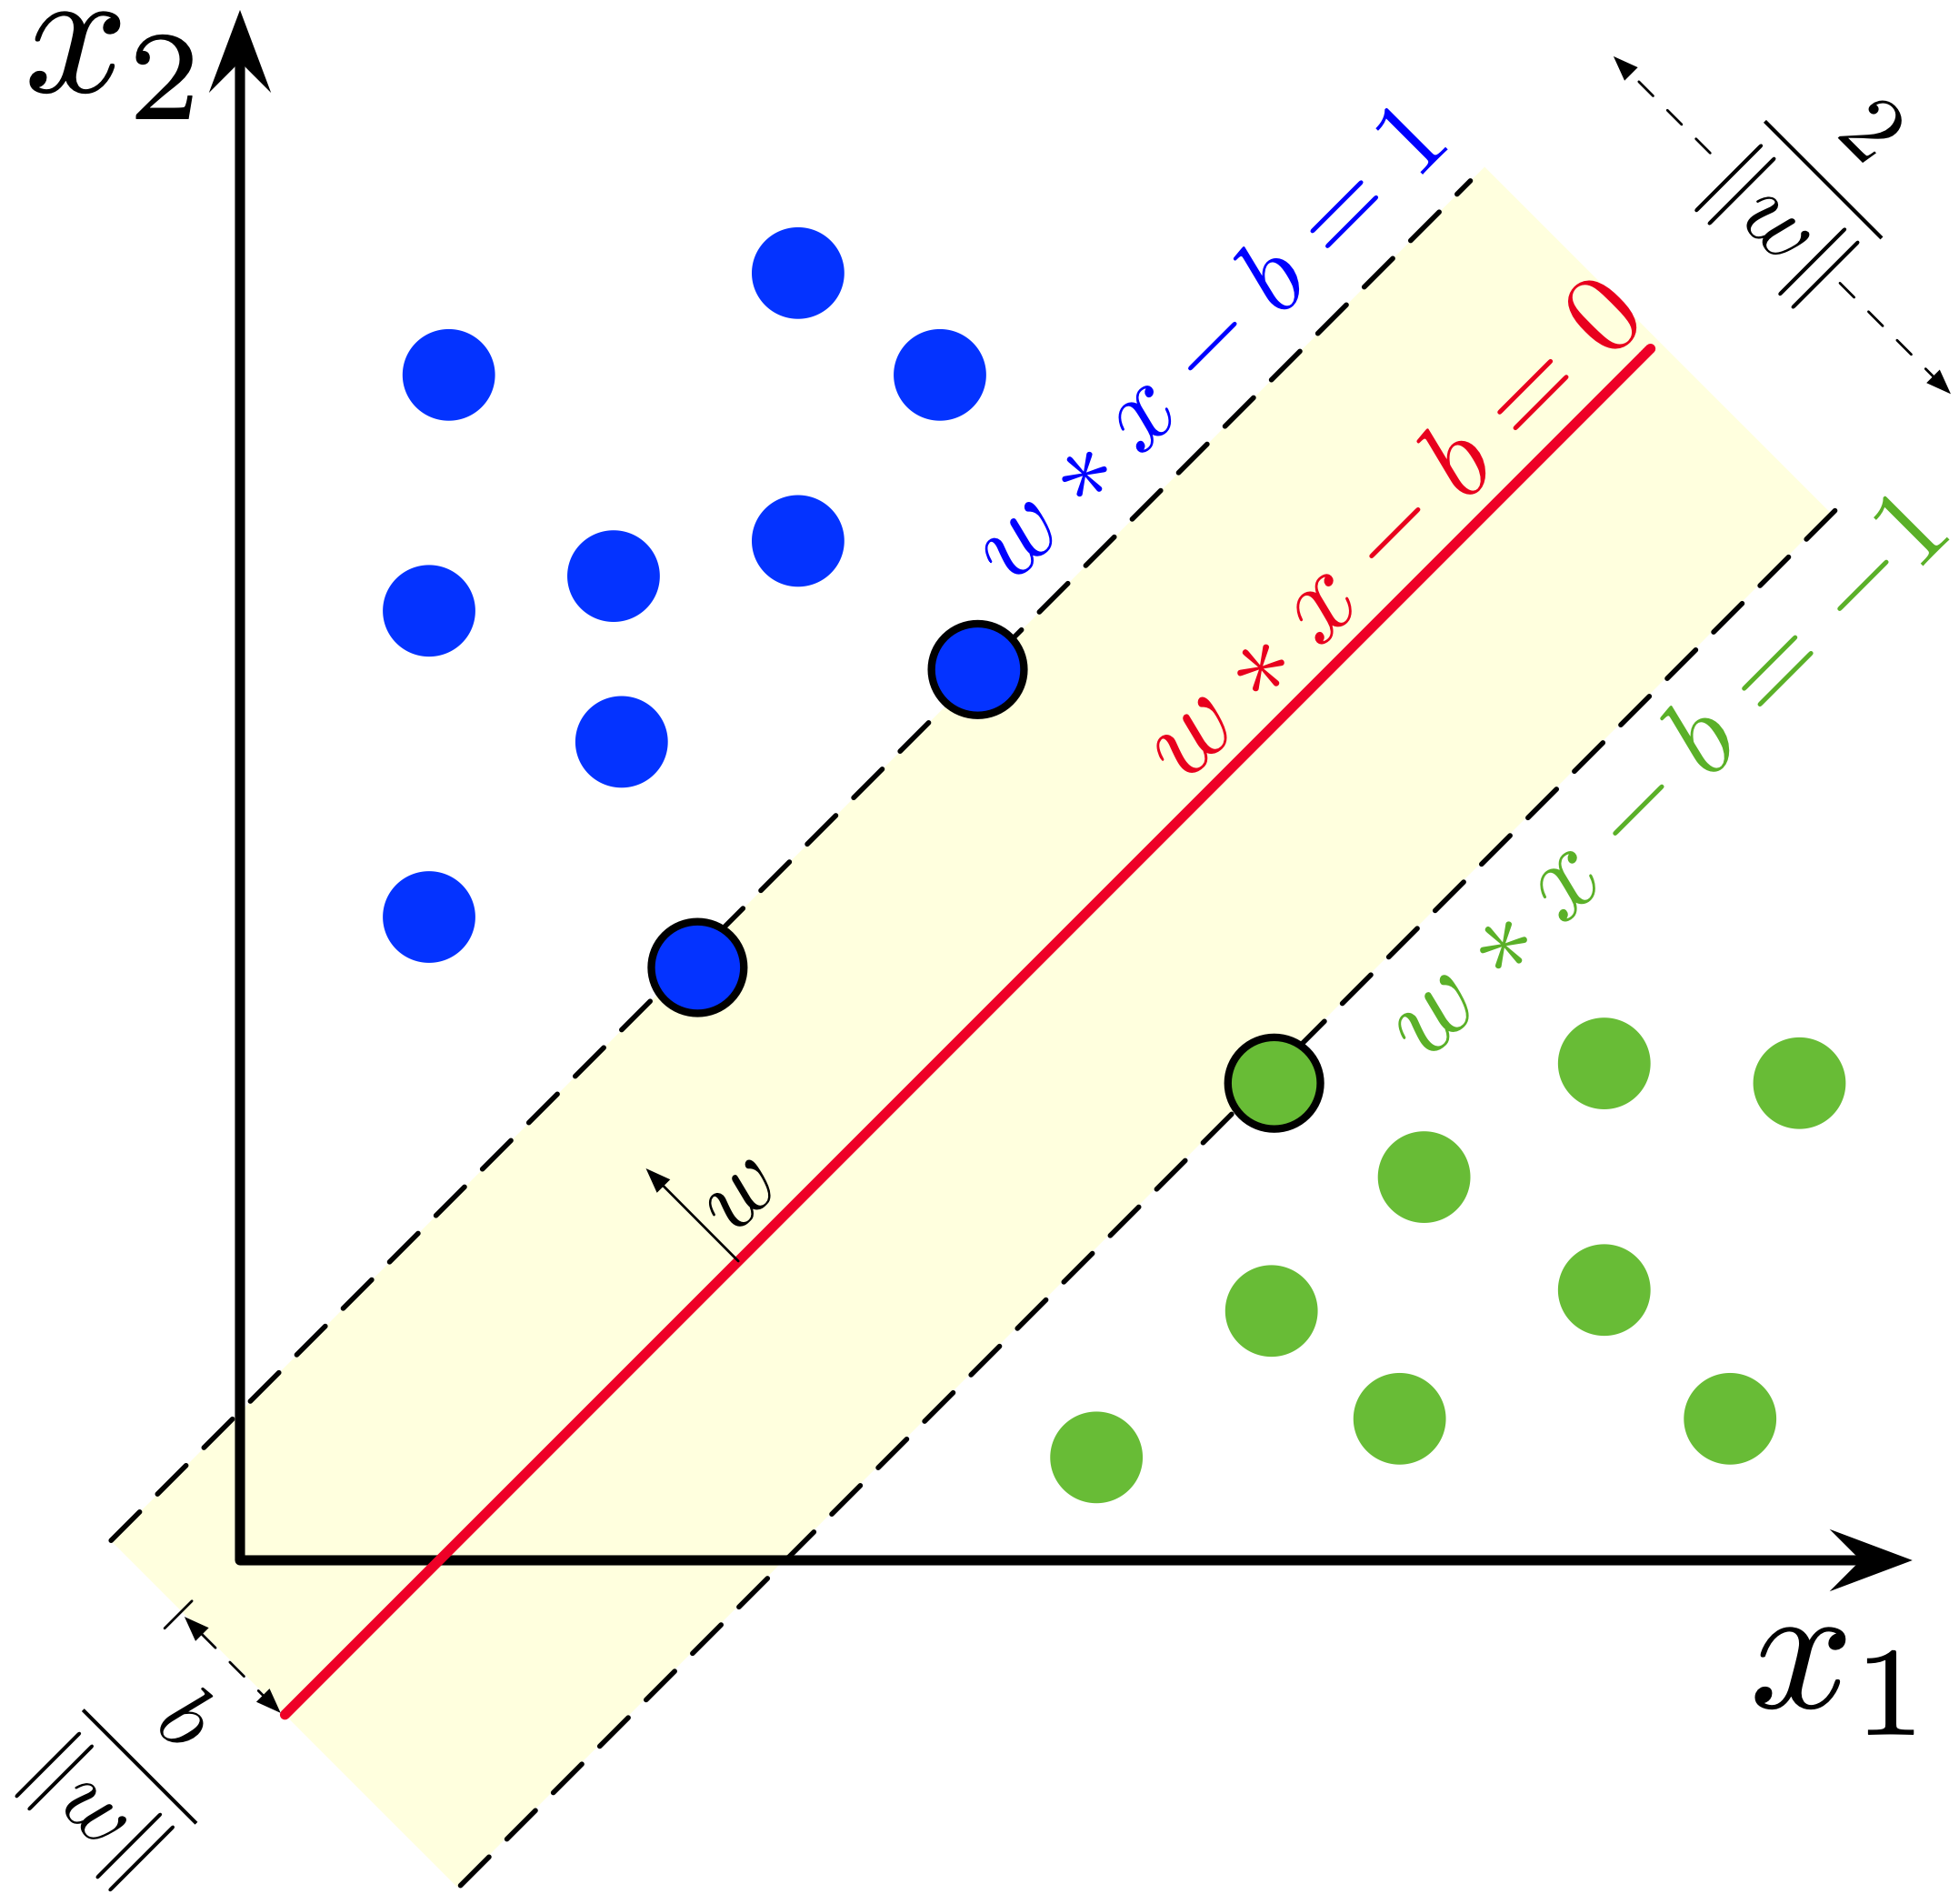
\includegraphics[height=\textheight]{FIGS_slides/SVM_margin}
    \end{minipage}
    \begin{minipage}{0.28\textwidth}
        Maximum-margin hyperplane and margins for an SVM trained with samples from two classes. Samples on the margin are the \textbf{support vectors}
    \end{minipage}
\end{frame}

\begin{frame}
    Any \textbf{hyperplane} can be written as the set of points $\mathbf{x}$ satisfying
    \[
        \bw^\mathsf{T} \bx - b = 0
    \]
    where $\bw$ is the (not necessarily normalized) \textbf{normal vector} to the hyperplane (if the hyperplane has equation $a_1z_1+\cdots+a_pz_p=c$, then $(a_1,\ldots,a_n)$ is normal to the hyperplane)
    % \vfill
    % This is much like \textbf{Hesse normal form}, except that $\mathbf{w}$ is not necessarily a unit vector
    \vfill
    The parameter $b/\|\bw\|$ determines the offset of the hyperplane from the origin along the normal vector $\bw$
    \vfill
    Remark: a hyperplane defined thusly is not a subspace of $\IR^p$ unless $b=0$. We can of course transform the data so that it is...
\end{frame}

\begin{frame}{Linearly separable points}
    Let $X_1$ and $X_2$ be two sets of points in $\IR^p$ 
    \vfill
    Then $X_1$ and $X_2$ are \textbf{linearly separable} if there exist $w_{1}, w_{2},..,w_{p}, k\in\IR$ such that 
    \begin{itemize}
        \item every point $x \in X_1$ satisfies $\sum^{p}_{i=1} w_{i}x_{i} > k$ 
        \item every point $x \in X_2$ satisfies $\sum^{p}_{i=1} w_{i}x_{i} < k$
    \end{itemize}
    where $x_{i}$ is the $i$th component of $x$
\end{frame}

\begin{frame}{Hard-margin SVM}
    If the training data is \textbf{linearly separable}, we can select two parallel hyperplanes that separate the two classes of data, so that the distance between them is as large as possible 
    \vfill
    The region bounded by these two hyperplanes is called the ``margin'', and the maximum-margin hyperplane is the hyperplane that lies halfway between them
    \vfill
    With a normalized or standardized dataset, these hyperplanes can be described by the equations
    \begin{itemize}
        \item $\mathbf{w}^\mathsf{T} \mathbf{x} - b = 1$ (anything on or above this boundary is of one class, with label 1) 
        \item $\mathbf{w}^\mathsf{T} \mathbf{x} - b = -1$ (anything on or below this boundary is of the other class, with label -1)
    \end{itemize}
\end{frame}

\begin{frame}
    Distance between these two hyperplanes is $2/\|\bw\|$
    \vfill
    $\Rightarrow$ to maximize the distance between the planes we want to minimize $\|\bw\|$
    \vfill
    The distance is computed using the distance from a point to a plane equation
    \vfill
    We must also prevent data points from falling into the margin, so we add the following constraint: for each $i$ either
    \[
        \mathbf{w}^\mathsf{T} \mathbf{x}_i - b \ge 1 \, , \text{ if } y_i = 1
    \]
    or
    \[
        \mathbf{w}^\mathsf{T} \mathbf{x}_i - b \le -1 \, , \text{ if } y_i = -1
    \]
    \vfill
    (Each data point must lie on the correct side of the margin)
\end{frame}

\begin{frame}
    This can be rewritten as
    \[
        y_i(\mathbf{w}^\mathsf{T} \mathbf{x}_i - b) \ge 1, \quad \text{ for all } 1 \le i \le n
    \]
    or
    \[
        y_i(\mathbf{w}^\mathsf{T} \mathbf{x}_i - b)-1\geq 0, \quad \text{ for all } 1 \le i \le n
    \]
    \vfill
    We get the optimization problem:
    \begin{quote}
        Minimize $\|\mathbf{w}\|$ subject to $y_i(\mathbf{w}^\mathsf{T} \mathbf{x}_i - b)-1 \ge 0$ for $i = 1, \ldots, n$
    \end{quote}
    \vfill
    The $\mathbf{w}$ and $b$ that solve this problem determine the classifier, $\mathbf{x} \mapsto \sgn(\mathbf{w}^\mathsf{T} \mathbf{x} - b)$ where $\sgn(\cdot)$ is the \textbf{sign function}.
\end{frame}

\begin{frame}   
    The maximum-margin hyperplane is completely determined by those $\bx_i$ that lie nearest to it
    \vfill
    These $\bx_i$ are the \textbf{support vectors}
\end{frame}

\begin{frame}{Writing the goal in terms of Lagrange multipliers}
    Recall that our goal is to
    \begin{quote}
        minimize $\|\mathbf{w}\|$ subject to $y_i(\mathbf{w}^\mathsf{T} \mathbf{x}_i - b)-1 \ge 0$ for $i = 1, \ldots, n$
    \end{quote}
    \vfill
    Using Lagrange multipliers $\lambda_1,\ldots,\lambda_n$, we have the function
    \[
        L_P:=F(\bw,b\lambda_1,\ldots,\lambda_n) =
        \frac 12\|\bw\|^2 -\sum_{i=1}^n \lambda_iy_i(\bx_i\bw+b)
        +\sum_{i=1}^n\lambda_i
    \]
    \vfill
    Note that we have as many Lagrange multipliers as there are data points. Indeed, there are that many inequalities that must be satisfied
    \vfill 
    The aim is to minimise $L_p$ with respect to $\bw$ and $b$ while the derivatives of $L_p$ w.r.t. $\lambda_i$ vanish and the $\lambda_i\geq 0$, $i=1,\ldots,n$
\end{frame}

\begin{frame}{Lagrange multipliers}
    We have already seen Lagrange multipliers, when we were studying PCA
    \vfill
\end{frame}

\begin{frame}{Maximisation using Lagrange multipliers (V1.0)}
    We want the max of $f(x_1,\ldots,x_n)$ under the constraint $g(x_1,\ldots,x_n)=k$
    \begin{enumerate}
    \item Solve
    \begin{align*}
    \nabla f(x_1,\ldots,x_n) &= \lambda\nabla g(x_1,\ldots,x_n) \\
    g(x_1,\ldots,x_n) &= k
    \end{align*}
    where $\nabla=(\frac{\partial}{\partial x_1},\ldots,\frac{\partial}{\partial x_n})$ is the \textbf{gradient operator}
    \item Plug all solutions into $f(x_1,\ldots,x_n)$ and find maximum values (provided values exist and $\nabla g\neq \b0$ there)
    \end{enumerate}
    \vfill
    $\lambda$ is the \textbf{Lagrange multiplier}
\end{frame}
    
    
\begin{frame}{The gradient}
    $f:\IR^n\to\IR$ function of several variables, $\nabla=\left(\frac{\partial}{\partial x_1},\ldots,\frac{\partial}{\partial x_n}\right)$ the gradient operator
    \vfill
    Then
    \[
    \nabla f = \left(
    \frac{\partial}{\partial x_1}f,\ldots,
    \frac{\partial}{\partial x_n}f
    \right)
    \]
    \vfill
    So $\nabla f$ is a \emph{vector-valued} function, $\nabla f:\IR^n\to\IR^n$; also written as
    \[
    \nabla f = f_{x_1}(x_1,\ldots,x_n)\be_1+\cdots f_{x_n}(x_1,\ldots,x_n)\be_n
    \]
    where $f_{x_i}$ is the partial derivative of $f$ with respect to $x_i$ and $\{\be_1,\ldots,\be_n\}$ is the standard basis of $\IR^n$
\end{frame}

\begin{frame}{Lagrange multipliers (V2.0)}
        However, the problem we were considering then involved a single multiplier $\lambda$
        \vfill
        Here we want $\lambda_1,\ldots,\lambda_n$
\end{frame}

\begin{frame}{Lagrange multiplier theorem}
    \begin{theorem}
        Let $f\colon\mathbb{R}^n \rightarrow \mathbb{R}$ be the objective function, $g\colon\mathbb{R}^n \rightarrow \mathbb{R}^c $ be the constraints function, both being $C^1$.
        Consider the optimisation problem
        \begin{align*}
            \text{maximize}\ f(x) \\
            \text{subject to}\ g(x) = 0                 
        \end{align*}
        Let $x^*$ be an optimal solution to the optimization problem, such that $\operatorname{rank} (Dg(x^*)) = c < n$, where $Dg(x^*)$ denotes the matrix of partial derivatives
        \[
            \left[{\partial g_j}/{\partial x_k}\right]  
        \]
        Then there exists a unique Lagrange multiplier $\lambda^* \in \mathbb{R}^c$ such that
        \[
            Df(x^*) = \lambda^{*T}Dg(x^*)
        \]
    \end{theorem}
\end{frame}

\begin{frame}{Lagrange multipliers (V3.0)}
    Here we want $\lambda_1,\ldots,\lambda_n$
    \vfill
    But we also are looking for $\lambda_i\geq 0$
    \vfill 
    So we need to consider the so-called Karush-Kuhn-Tucker (KKT) conditions
\end{frame}

\begin{frame}{Karush-Kuhn-Tucker (KKT) conditions}
    Consider the optimisation problem
    \begin{align*}
        \text{maximize}\ f(x) \\
        \text{subject to}& \quad g_i(x) \leq 0  \\
        &\quad h_i(x)=0               
    \end{align*}
    Form the Lagrangian
    \[
        L(\bx,\mu,\lambda) = f(\bx)+\mu^T\bg(\bx)+\lambda^T\bh(\bx)
    \]
    \begin{theorem}
        If $(\mathbf{x}^{\ast},\mathbf{\mu}^\ast)$ is a \emph{saddle point} of $L(\mathbf{x},\mathbf{\mu})$ in $\mathbf{x} \in \mathbf{X}$, $\mathbf{\mu} \geq \mathbf{0}$, then $\mathbf{x}^{\ast}$ is an optimal vector for the above optimization problem. Suppose that $f(\mathbf{x})$ and $g_i(\mathbf{x})$, $i = 1, \ldots, m$, are \emph{convex} in $\mathbf{x}$ and that there exists $\mathbf{x}_{0} \in \mathbf{X}$ such that $\mathbf{g}(\mathbf{x}_{0}) < 0$. Then with an optimal vector $\mathbf{x}^{\ast}$ for the above optimization problem there is associated a non-negative vector $\mathbf{\mu}^\ast$ such that $L(\mathbf{x}^{\ast},\mathbf{\mu}^\ast)$ is a saddle point of $L(\mathbf{x},\mathbf{\mu})$
    \end{theorem}
\end{frame}

\begin{frame}{KKT conditions}
    \begin{align*}
        \frac{\partial}{\partial w_\nu}L_P &=
        w_\nu-\sum_{i}^n\lambda_iy_ix_{i\nu}=0
        \qquad\nu=1,\ldots,p \\
        \frac{\partial}{\partial b}L_P &=
        -\sum_{i=1}^n \lambda_iy_i = 0 \\
        y_i(\bx_i^T\bw+b)-1 &\geq 0\qquad i=1,\ldots,n \\
        \lambda_i &\geq 0\qquad i=1,\ldots,n \\
        \lambda_i(y_i(\bx_i^T\bw+b)-1) &=0\qquad i=1,\ldots,n \\
    \end{align*}
\end{frame}


    
\begin{frame}{Soft-margin SVM}
    To extend SVM to cases in which the data are not linearly separable, the \textbf{hinge loss} function is helpful
    \[
        \max\left(0, 1 - y_i(\mathbf{w}^\mathsf{T} \mathbf{x}_i - b)\right)
    \]
    \vfill
    $y_i$ is the $i$th target (i.e., in this case, 1 or -1), and $\mathbf{w}^\mathsf{T} \mathbf{x}_i - b$ is the $i$-th output
    \vfill
    This function is zero if the constraint is satisfied, in other words, if $\mathbf{x}_i$ lies on the correct side of the margin
    \vfill 
    For data on the wrong side of the margin, the function's value is proportional to the distance from the margin
\end{frame}

\begin{frame}
   
    The goal of the optimization then is to minimize
    
    \[ 
        \lambda \lVert \mathbf{w} \rVert^2 +\left[\frac 1 n \sum_{i=1}^n \max\left(0, 1 - y_i(\mathbf{w}^\mathsf{T} \mathbf{x}_i - b)\right) \right]
    \]
    
    where the parameter $\lambda > 0$ determines the trade-off between increasing the margin size and ensuring that the $\mathbf{x}_i$ lie on the correct side of the margin
    \vfill
    Thus, for sufficiently small values of $\lambda$, it will behave similar to the hard-margin SVM, if the input data are linearly classifiable, but will still learn if a classification rule is viable or not
\end{frame}

\end{document}
